\documentclass[a4paper,11pt,onepage]{article}

\usepackage[utf8]{inputenc}
\usepackage{graphicx}
\usepackage{amsmath}
\usepackage{amsfonts}
\usepackage{a4wide}
\usepackage[colorlinks=true]{hyperref}
\usepackage{mathtools}

\newcommand{\hc}{h_\mathrm{c}}
\newcommand{\hp}{h_\mathrm{p}}
\newcommand{\hmax}{h_\mathrm{max}}
\newcommand{\Fc}{F_\mathrm{c}}
\newcommand{\Fmax}{F_\mathrm{max}}
\newcommand{\Ap}{A_\mathrm{p}}
\newcommand{\Hit}{H_\mathrm{IT}}
\newcommand{\Eit}{E_\mathrm{IT}}
\newcommand{\Er}{E_\mathrm{r}}
\newcommand{\nui}{\nu_\mathrm{i}}
\newcommand{\Ei}{E_\mathrm{i}}
\newcommand{\cov}{\mathrm{cov}}
\newcommand{\ahp}{a_\mathrm{\hp}}
\newcommand{\bhp}{b_\mathrm{\hp}}
\newcommand{\ddp}[2]{\frac{\partial #1}{\partial #2}}
\newcommand{\depsdm}{\ddp{\varepsilon}{m}}
\newcommand{\Sload}{S_{\mathrm{load}}} 
\newcommand{\Sunload}{S_{\mathrm{unload}}}
\newcommand{\kl}{k_{\mathrm{load}}}
\newcommand{\ql}{q_{\mathrm{load}}}
\newcommand{\ku}{k_{\mathrm{unload}}}
\newcommand{\qu}{q_{\mathrm{unload}}}

\title{\textsc{Niget: NanoIndentation \\ General Evaluation Tool}}
\author{Anna Charvátová Campbell, Radek Šlesinger, Petr Grolich \\ Czech Metrology Institute}

\begin{document}
\maketitle

\tableofcontents

\section{About}

Nanoindentation instruments often include data processing software, however, this may not be sufficient. 
The desired evaluation method may not implemented, the implementations may not be suitable for the given physical problem, 
the description of the implementation may be insufficient or more information about uncertainties is sought for. \\
This toolbox aims to fill this gap (at least partly). It is open-source, so the implementation can be checked by the user. It can also be easily expanded to include also other evaluation methods.
Uncertainties are provided both in the standard framework of uncertainty propagation and also using Monte Carlo simulations.

Visit Niget home page at \url{http://nanometrologie.cz/niget}.


%  System requirements, compilation, installation
%------------------ System requirements, installation ----------------------
\section{System requirements, compiling, and installation}

Niget sources as well as binaries for 32-bit Windows systems can be downloaded from its home page at \url{http://nanometrologie.cz/niget}.
The software is written mainly in C language using GTK+ (version 2) toolkit (\url{http://www.gtk.org}) and libraries from Gwyddion data analysis software (\url{http://gwyddion.net}). 
Some tools (Oliver-Pharr ODR, Hertz ODR, Two slopes, and Stiffness) use orthogonal distance regression (ODR) which includes Fortran code from ODRPACK95 project, available at \url{http://www.netlib.org/toms/869.zip}.

\subsection{Linux}

There are no distribution packages available, and users are supposed to compile Niget from source.

\paragraph{Requirements}

\begin{enumerate}
\item C compiler (preferably GNU gcc or Intel icc)
\item (optional) Fortran compiler (preferably GNU gfortran or Intel ifort)
\item CMake
\item GNU Make or compatible
\item pkg-config
\item GTK2 (and its dependences), including development libraries
\item (preferable) Gwyddion development libraries (see \url{http://gwyddion.net/download.php} for distribution-specific instructions; FFTW3 and GtkGLExt development libraries may be also required as dependences)
\end{enumerate}

If paths to Gwyddion libraries and includes are not found by CMake or provided by user, a recent version of Gwyddion is automatically downloaded and built. Please that this does not include any additional tools or libraries which might be required by Gwyddion; these must be installed manually according to the installation instructions of Gwyddion.

\paragraph{Compiling with CMake}

In the Niget source directory, proceed as follows:

\begin{enumerate}
\item \texttt{mkdir build} (out-of-tree builds are preferred with CMake)
\item \texttt{cd build}
\item \texttt{cmake ..} (CMake looks for compilers and libraries, and configures the build)
\item \texttt{make}
\end{enumerate}

This compiles Niget using default configuration. If CMake finds a suitable Fortran compiler, ODRPACK95 will be compiled and ODR-based tools enabled. Optional configuration parameters can be set by adding \texttt{-D OPTION=VALUE} to the \texttt{cmake} command (\texttt{cmake -D OPTION1=VALUE1 \dots\ -D OPTIONn=VALUEn ..}). Presently available options are:

\begin{enumerate}
\item \texttt{DEBUG} -- \texttt{ON} (default) / \texttt{OFF}: make debug build
\item \texttt{VERBOSE} -- \texttt{ON} / \texttt{OFF} (default): increase verbosity of some tools for debugging purposes
\end{enumerate}

Specific compilers can be provided using \texttt{CC} and \texttt{FC} environment variables, e.g. \texttt{CC=icc FC=ifort cmake ..} to use Intel compilers. After running CMake, the options above are stored into CMake's cache in the build directory, and need not be specified with further CMake runs (or have to be specified explicitly if a change is desired). Note: until the code is sufficiently tested, \texttt{DEBUG} is \texttt{ON} by default, and release build must be triggered manually.

After the software compiles successfully, the \texttt{niget} binary, created in the build directory, can be run.


\subsection{Windows}

Niget Windows 32-bit binaries are distributed in a single zip-file, which contains all the required libraries.
% (If the software does not run, you might need to install the Visual C++ Redistributable for Visual Studio 2015, available at \url{https://www.microsoft.com/en-us/download/details.aspx?id=48145}.)
This is the preferred way for Windows users to start using Niget.

% \subsubsection{Microsoft Visual Studio}

% Niget can be compiled natively on Windows platforms. A solution for Microsoft Visual Studio 2015 is provided in \texttt{msvc2015/indent-toolbox.sln}. 
% Since this Visual Studio version does not provide a Fortran compiler, the ODR dependent tools are excluded into a separate project, which can be compiled as a dynamic link library using Intel Fortran compiler. Anyway, due to GTK2 and Gwyddion development libraries being needed for compilation, we discourage the users from compiling from source on Windows.

% \paragraph{Requirements}

% \begin{enumerate}
% \item Microsoft Visual Studio 2015
% \item (Optional) Intel Fortran compiler
% \item GTK2 Windows bundle (\url{http://gtk-win.sourceforge.net/home})
% \item Gwyddion development libraries; see \url{http://gwyddion.net/documentation/user-guide-en/installation-compiling-msvc.html} for instructions on compiling Gwyddion on Windows
% \end{enumerate}

\subsubsection{MinGW suite}

Compiling using CMake and MinGW suite in MSYS2 environment has been tested and is currently used to provide the Windows builds of Niget. Unfortunately, no straightforward procedure is available at the moment.

% -G "Unix Makefiles"
% -DGTK2_GDKCONFIG_INCLUDE_DIR=/mingw32/lib/gtk-2.0/include -DGTK2_GLIBCONFIG_INCLUDE_DIR=/mingw32/lib/glib-2.0/include - zahrnuto v cmakelists, ale musely se pridat zacatky cest



\newpage


% Main window 
%---------------- Main window ---------------------
\section{Main Window}

Niget's graphical user interface (GUI) can be started by running the \texttt{niget} (\texttt{niget.exe}) executable. Using two optional parameters \emph{filename} and \emph{fileformat} (currently available options: \emph{niget}, \emph{unht}, \emph{hysitron}), a file of a given type is opened on application start by running \texttt{niget -f fileformat filename}.

The main window shows all currently available methods as different tabs and a row of general function buttons. The tabs are inactive at the start of the program and get activated when a file is opened.

\begin{figure}[ht]
  \centering
  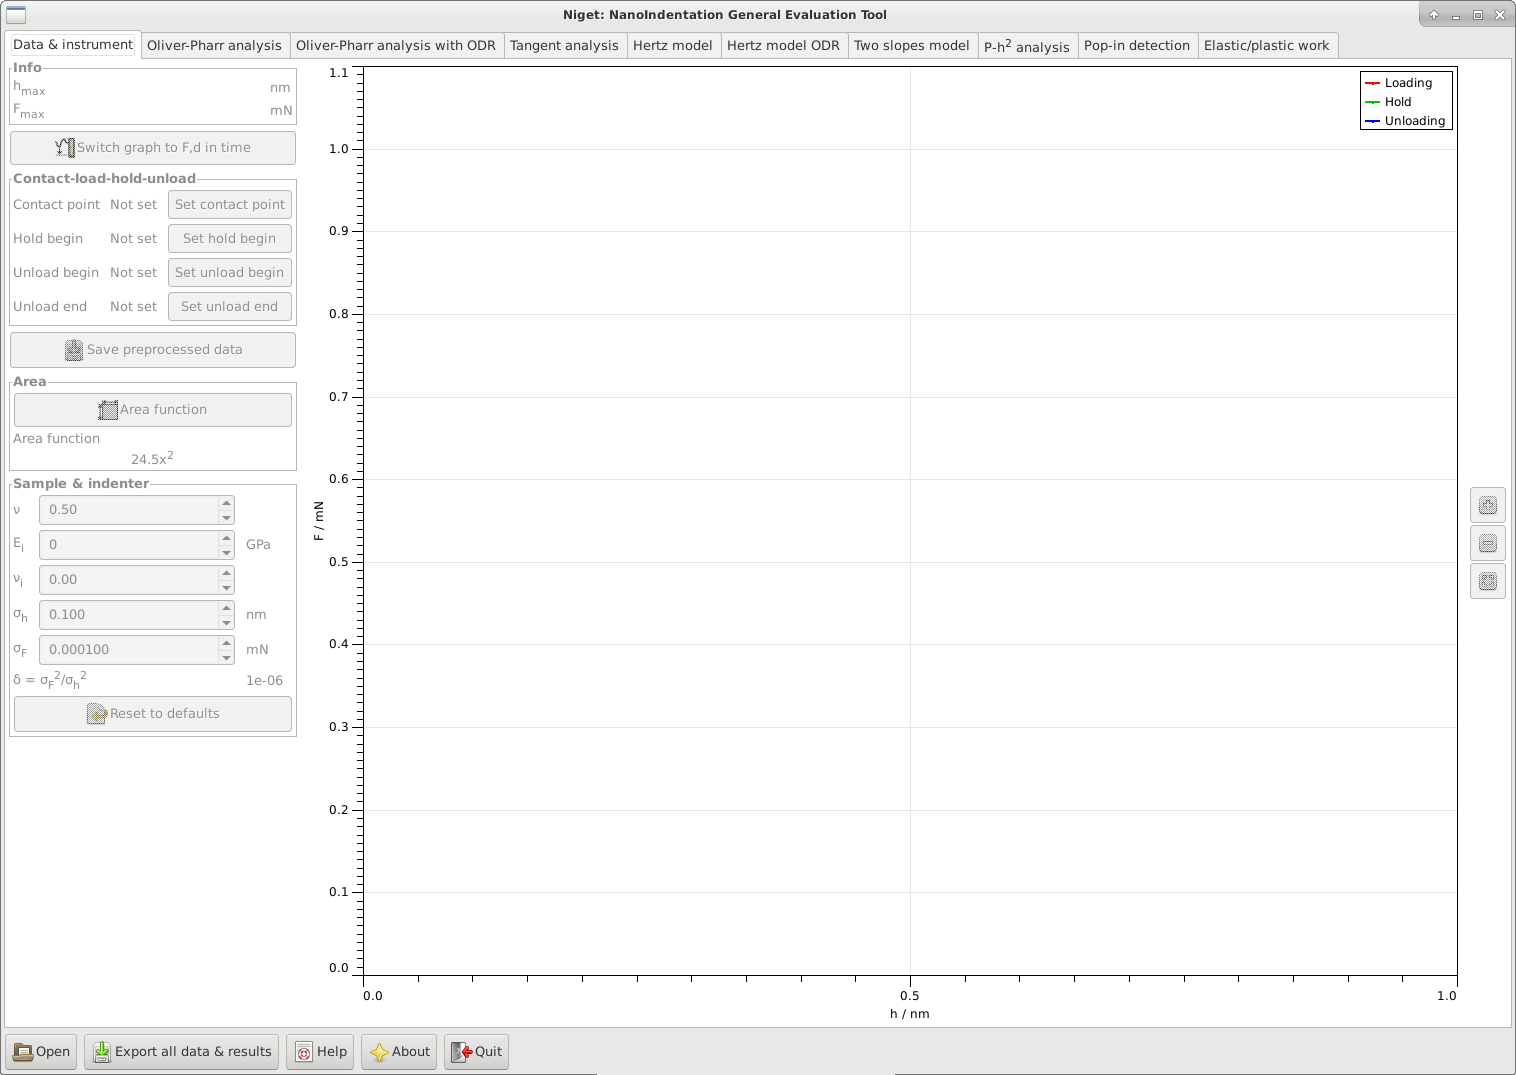
\includegraphics[width=\textwidth]{images/screen-main}
  \caption{Main window}
\end{figure}

The buttons are:
\begin{itemize}
 \item \emph{Open:} Load a file in a chosen format. Currently, only files of one of the predefined plain-text formats. can be opened. 
 Each file should contain only one loading-unloading curve. Files with more than one indentation should load as well, but the behaviour may be ``surprising''. Currently, only the decimal point is supported as the decimal mark.
 Lines that do not correspond to the given format, because they are, e.g., empty or hold comments, are skipped. \\
 WARNING: The units MUST agree with the given format or you will get nonsense numerical results! 
 
 \begin{itemize}
 \item[-] \verb|Time (s)  Depth (nm)  Load (mN)|: first three columns correspond to time (which is skipped), depth in nm and load in mN.
 \item[-] \verb|Time (s)  Depth (nm)  Load (uN)|: first three columns correspond to time (which is skipped), depth in nm and load in $\mu$N.
 \item[-] \verb|Depth (nm)  Load (uN)|: first two columns correspond to depth in nm and load in $\mu$N.
 \item[-] \verb|Depth (nm)  Load (mN)|: first two columns correspond to depth in nm and load in mN.
 \item[-] \verb|Load (mN)  Depth (nm)|: first two columns correspond to load in mN and depth in nm.
 \item[-] \verb|Load (uN)  Depth (nm)|: first two columns correspond to load in $\mu$N and depth in nm.
 \item[-] \verb|Niget|: native format of Niget.
 \end{itemize}
 The file cannot be loaded if it's not in the given format or if it contains \verb|inf| or \verb|nan| values. The data are supposed to be sufficiently comprehensive in order to define the contact point as well the loading and unloading part.

 \item \emph{Export all data \& results:} Save the processed indentation data and  results from all methods. The user chooses a basename to which a suffix is appended for each method. A file is created even if there are no meaningful results for a method. 
                    %Results of uncertainty analysis and Monte Carlo calculations are saved as well.
 \item \emph{Help:} Open HTML documentation in an associated browser.
 \item \emph{About:} Display additional information about the software.
 \item \emph{Quit:} Exit the program.
\end{itemize}

Note that when the program exits (either by pressing \emph{Quit} or closing the main window), no results are saved. \\
The program keeps its own few settings for user comfort. These are saved in \verb|niget_settings.cfg| in the user configuration directory. 


%Data and area 
%------------------ Data, time regime, area ---------------------------
\section{Data \& area}

In this tab the user can set the contact point as well as other important points of the indentation process, mechanical properties of the tip and sample, indenter noise and define the area function.
After successfully loading a file, the software creates the force-distance diagram from the data, and attempts to automatically detect the loading, hold and unloading parts of the data.

\begin{figure}[ht]
  \centering
  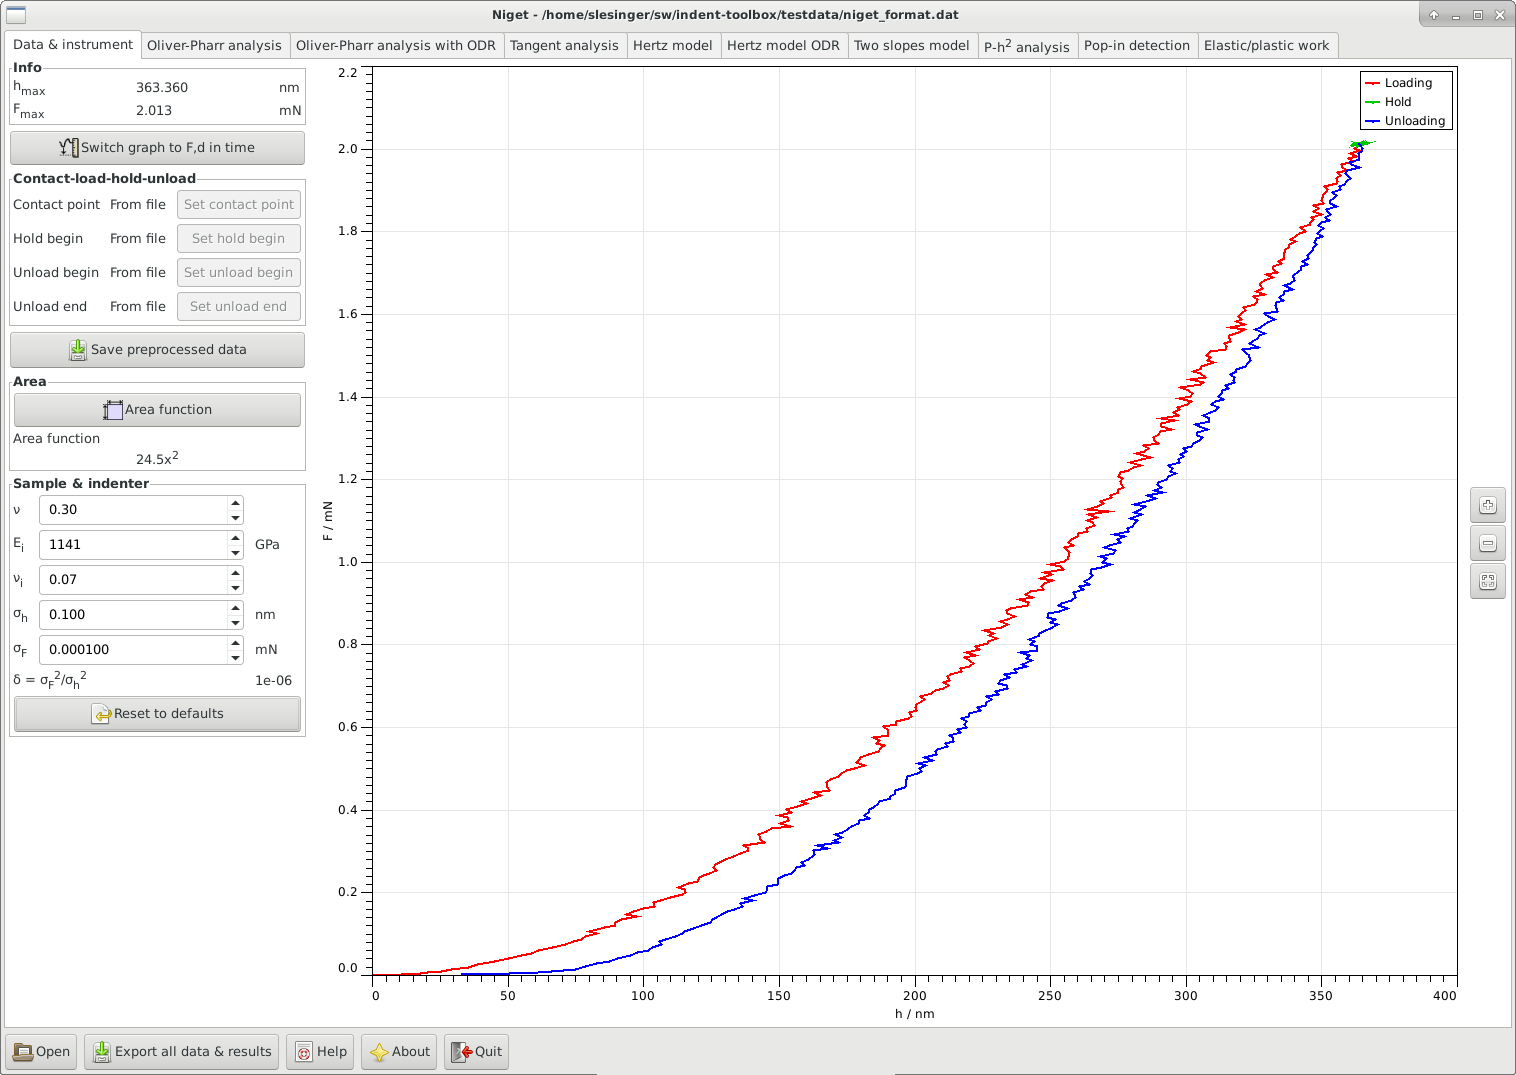
\includegraphics[width=\textwidth]{images/screen-fd}
  \caption{Force-distance diagram after automatic split}
\end{figure}

\begin{figure}[ht]
  \centering
  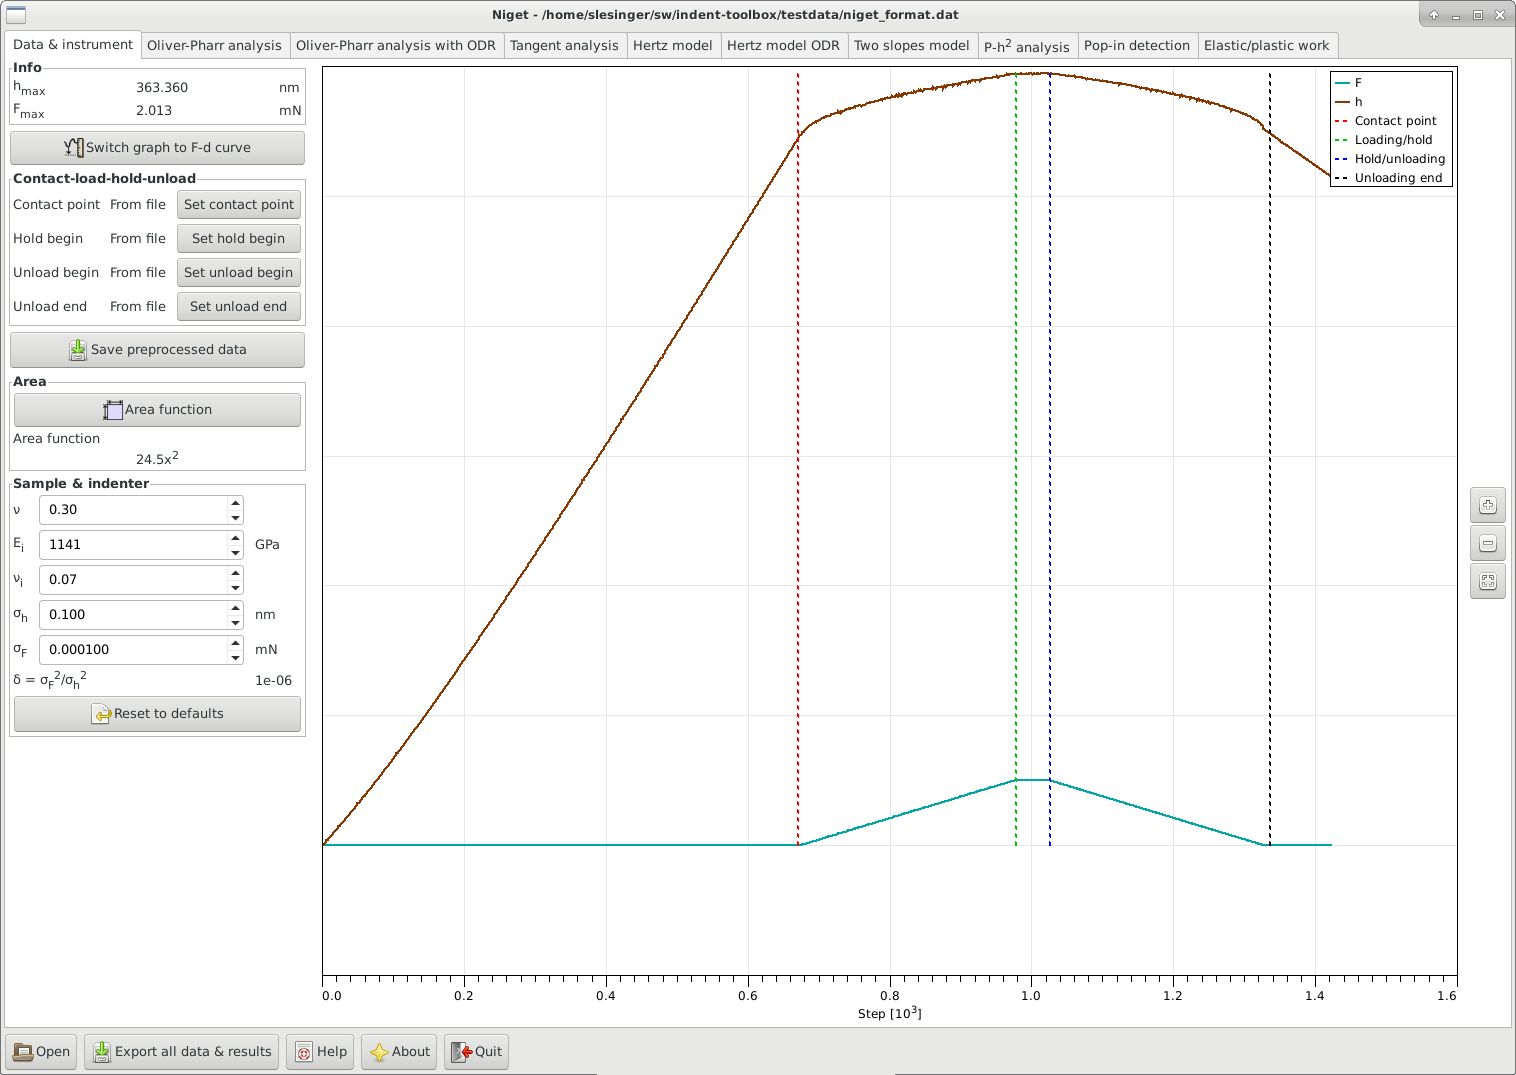
\includegraphics[width=\textwidth]{images/screen-fdtime}
  \caption{Manual definition of points in force-distance in time view}
\end{figure}

\subsection{Window}
The window consists of the following:
\begin{itemize}
 \item \emph{Info} displays the maximum depth and force during the indentation determined as in section \ref{contact_max}. 
 \item \emph{Switch graph to \dots} switches between two display modes: force as a function of depth (F-d) and force and depth as functions of the (pseudo)time (F,d-t). The index of the data point is used instead of the real time, which is not read from the file.
 In the second case, both curves are displayed dimensionless, and scaled just to provide good visual resolution.
 \item \emph{Contact-load-hold-unload} Allows to manually split the data into the loading, hold and unloading parts:
 \begin{itemize}
 \item[-] Contact point: determines the beginning of the loading curve. The depth and force at this point $h_c$ and $F_c$ are subtracted from the loading-unloading curves.
 \item[-] Hold begin
 \item[-] Unload begin 
 \item[-] Unload end: define the end of the unloading part. By default, the data are truncated at zero depth.
\end{itemize}
  Whether the point was set automatically or manually is shown. Note, that if the division of the data into the different parts is changed, all analysis results are deleted!
 \item \emph{Save preprocessed data} saves the data including the selected split of the data in the native format Niget. 
 \item \emph{Area}
 \begin{itemize}
 \item[-] Area function button: opens a separate dialog for the definition of the area function, see \ref{area}
 \item[-] displays the area function used currently.
 \end{itemize}
  \item \emph{Sample \& indenter}
    The parameters here are Poisson's value of the sample, Young's modulus of the indenter, Poisson's value of the indenter and the noise of the displacement and load sensors. The default values are 0.3, 1141~GPa, and 0.07. 
    The first is a reasonable estimate of the often unknown Poisson's value for many materials, the other two values are the literature values for diamond which is a common indenter tip material. 
    The noise of the sensors is used for the fitting procedures and for the uncertainty analysis.
    These values are saved in settings and can be reset to their default values.
\item \emph{Graph}  displays the indentation curve.  Stepwise zooming/unzooming can be performed by selecting a range with the mouse and pressing the \emph{Zoom}/ \emph{Unzoom} buttons. The graph is restored to its original size by the \emph{Restore} button.
The zooming procedure is independent in the two regimes (F-d vs. F,d-t).
\end{itemize}

\subsection{Maximum depth and force} \label{contact_max}
The maximum force $\Fmax$ is the maximum force value found in the unloading data. The maximum depth $\hmax$ is the corresponding depth, NOT the maximum depth value!

\subsection{Area function} \label{area}
The area function can be given either in form of a polynomial of the form
\begin{equation} \label{eq:Aphc}
A(h) = c_2 h^2 + c_1 h + c_{1/2} h^{1/2} + c_{1/4} h^{1/4} + c_{1/8} h^{1/8} + c_{1/16} h^{1/16},
\end{equation}
or a raw data file can be loaded, which will be (linearly) interpolated in subsequent calculations. The format of the area data file MUST be two columns: first column depth in nm, second column area in nm$^2$.\\ 
The area function is shown for user information. A warning is issued if a raw data file is used and any of the methods extrapolates the area. 
The coefficients of a polynomial area function are saved in the settings file. 

For specific formats, the coefficients can also be loaded directly from a file. 
Currently, this should work for an \verb|.ara| file (as exported from a Hysitron instrument) or for an \verb|.ind| file (as exported from a UNHT Anton Paar instrument). 
This is under testing and may not work correctly for other versions. 

\begin{figure}[h]
  \centering
  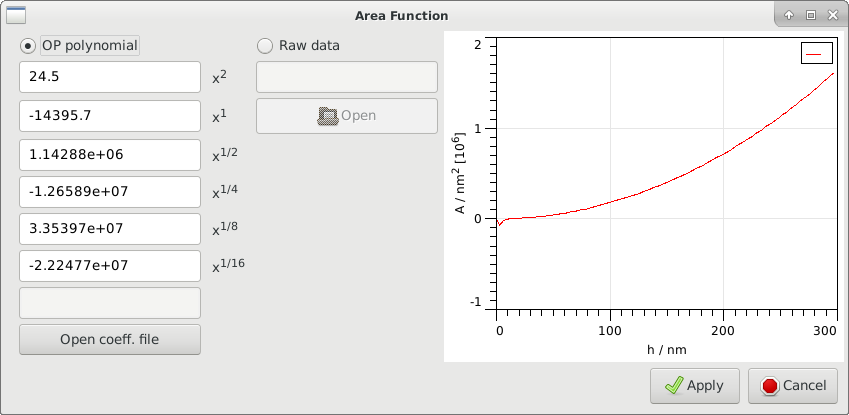
\includegraphics[width=.6\textwidth]{images/screen-area}
  \caption{Area function dialog}
\end{figure}


%  simple Oliver Pharr  
%-------------- Oliver Pharr   -------------------------------%
\section{Oliver Pharr}
For a definition of the Oliver Pharr method see \cite{OliverPharr}. \\

\begin{figure}[ht]
  \centering
  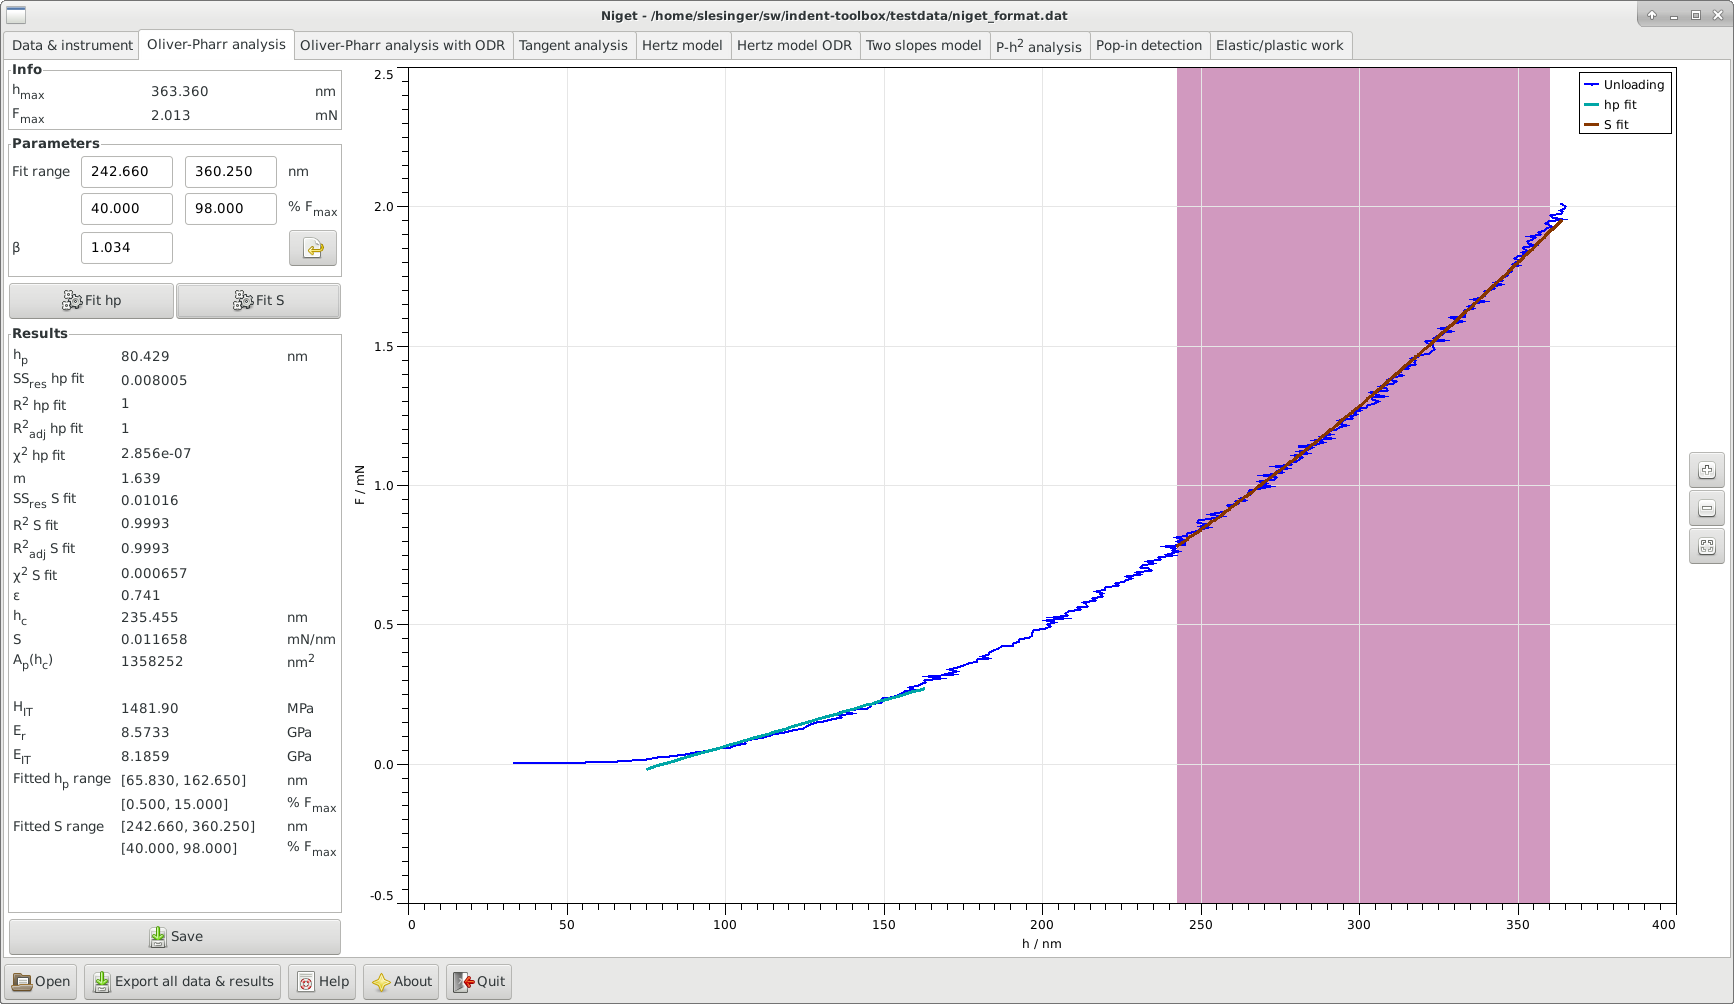
\includegraphics[width=\textwidth]{images/screen-op}
  \caption{Oliver-Pharr analysis}
\end{figure}

\subsection{Window}
The window consists of several blocks:
\begin{itemize}
 \item \emph{Info} displays the maximum depth and force during the indentation
 \item \emph{Parameters} shows the selected range in nm and in \% of the maximum force, and the correction $\beta$. 
        \begin{itemize}
          \item[-] The fitting range can be selected either using the mouse or typing in the range entries. The range can be defined either in nm or in percent of the maximum force. 
                   It is often recommended to use the range 0.5--15~\% F$_\mathrm{max}$ for the hp fit and 40--98~\% F$_\mathrm{max}$ for the S fit, see section \ref{op_calc}.      
          \item[-] The parameter $\beta$ accounts for any deviations from the axisymmetric case and is used in the calculation of the reduced modulus in equation \eqref{eq:Er}. 
                   Currently, the default value is the value for three-sided pyramides $\beta = 1.034$. The value supplied by the user is saved in the settings and can be reset to its default value.
\end{itemize}
\item \emph{Fit} buttons for the two fits, see section \ref{op_calc} for details of the calculation.
\item \emph{Results} displays all results in the following order: the residual depth $\hp$, the power $m$ of the power law function, the parameter $\varepsilon$, 
       the contact depth  $\hc$, the slope $S$, the contact area $\Ap(\hc)$, the indentation hardness $H_{IT}$, the contact modulus $E_r$, the indentation modulus $E_{IT}$ and the ranges used for the fitting procedures.
       The variables are described in detail in section \ref{op_calc}.
 %\item \emph{Uncertainties} show the uncertainty analysis window, see section \ref{op_unc}.
 \item \emph{Save} save parameters and results to given file. 
 \item \emph{Graph} display the unloading curve and the fitted curves.  Stepwise zooming/unzooming can be performed by selecting a range with the mouse and pressing the \emph{Zoom}/ \emph{Unzoom} buttons. The graph is restored to its original size by the \emph{Restore} button.
\end{itemize}

\subsection{Procedure}\label{op_calc}
The standard calculation consists of three steps
\begin{enumerate}
 \item  The residual depth must be determined as the intersection of the unloading curve and the x-axis.
This is implemented by fitting a straight line using a Deming fit with $\delta = 1$, see section \ref{tls}. 
For a brief description of the Deming fit see section \ref{tls}
\begin{equation}
F = \ahp \hp + b_\mathrm{h_{p}} \label{eq:hp-fit}
\end{equation}

using total least squares. This fit is called the $\hp$ fit. The residual depth is calculated as 
\begin{equation} \label{eq:hp}
 \hp = -b_{\hp}/a_{\hp}. 
\end{equation}
The range of the data must be chosen adequately, the range 0.5--15 \% F$_\mathrm{max}$ is often a reasonable value. \\

\item The main part of the unloading curve is fitted by a power law function
\begin{equation}
F = \alpha (h - \hp)^m.
\end{equation}
This is converted to a total least squares fit in the variables using a Deming fit with $\delta =1 $, see section \ref{tls}
\begin{equation}
\log F = \log \alpha + m \log (h- \hp). \label{eq:m-fit}
\end{equation}
The range should not contain the lower part of the unloading range, a range of 40--98~\% F$_\mathrm{max}$ is recommended as a first guess.

\item The auxiliary parameter $\varepsilon$ is calculated from the power $m$
\begin{equation} \label{eq:eps}
\varepsilon = m \left(1-\frac{2(m-1) \Gamma\left(\frac{m}{2(m-1)}\right)}{\sqrt{\pi}\Gamma\left(\frac{1}{2(m-1)}\right)} \right),
\end{equation}
$\Gamma$ is the Gamma-function. \\
The contact depth is calculated as 
\begin{equation} \label{eq:hc}
	\hc=\hmax-\epsilon \frac{\Fmax}{S}
\end{equation}
and the slope at the maximum depth as
\begin{equation} \label{eq:S}
S=m \frac{ \Fmax}{\hmax-\hp}.
\end{equation}
\item 
The contact depth is used to evaluate the contact area $A(\hc)$.
This can be used to find the indentation hardness
\begin{equation}\label{eq:Hit}
\Hit=\frac{\Fmax}{A(\hc)}.
\end{equation}
and together with the slope to find the contact modulus
\begin{equation}\label{eq:Er}
\Er=\sqrt{\pi} \frac{S}{2 \beta \sqrt{A(\hc)}}.
\end{equation}
For a comparison with Young's modulus found in literature it is useful to calculate the indentation modulus $E_{IT}$ 
\begin{equation} \label{eq:Eit}
\Eit = \frac{1 - \nu^2}{1/\Er - (1 - \nui^2) / \Ei}.
\end{equation}
Here $\nu$ is the Poisson's value of the sample and $\nui$ and $\Ei$ are the Poisson's value and the modulus of the indenter. 
\end{enumerate} 


% Oliver Pharr ODR
%-------------- Oliver Pharr  ODR  -------

\section{Oliver Pharr with ODR}
For a definition of the Oliver Pharr method see \cite{OliverPharr}. \\ 
This method is shown unless the software was compiled without Fortran support.  \\

\begin{figure}[ht]
  \centering
  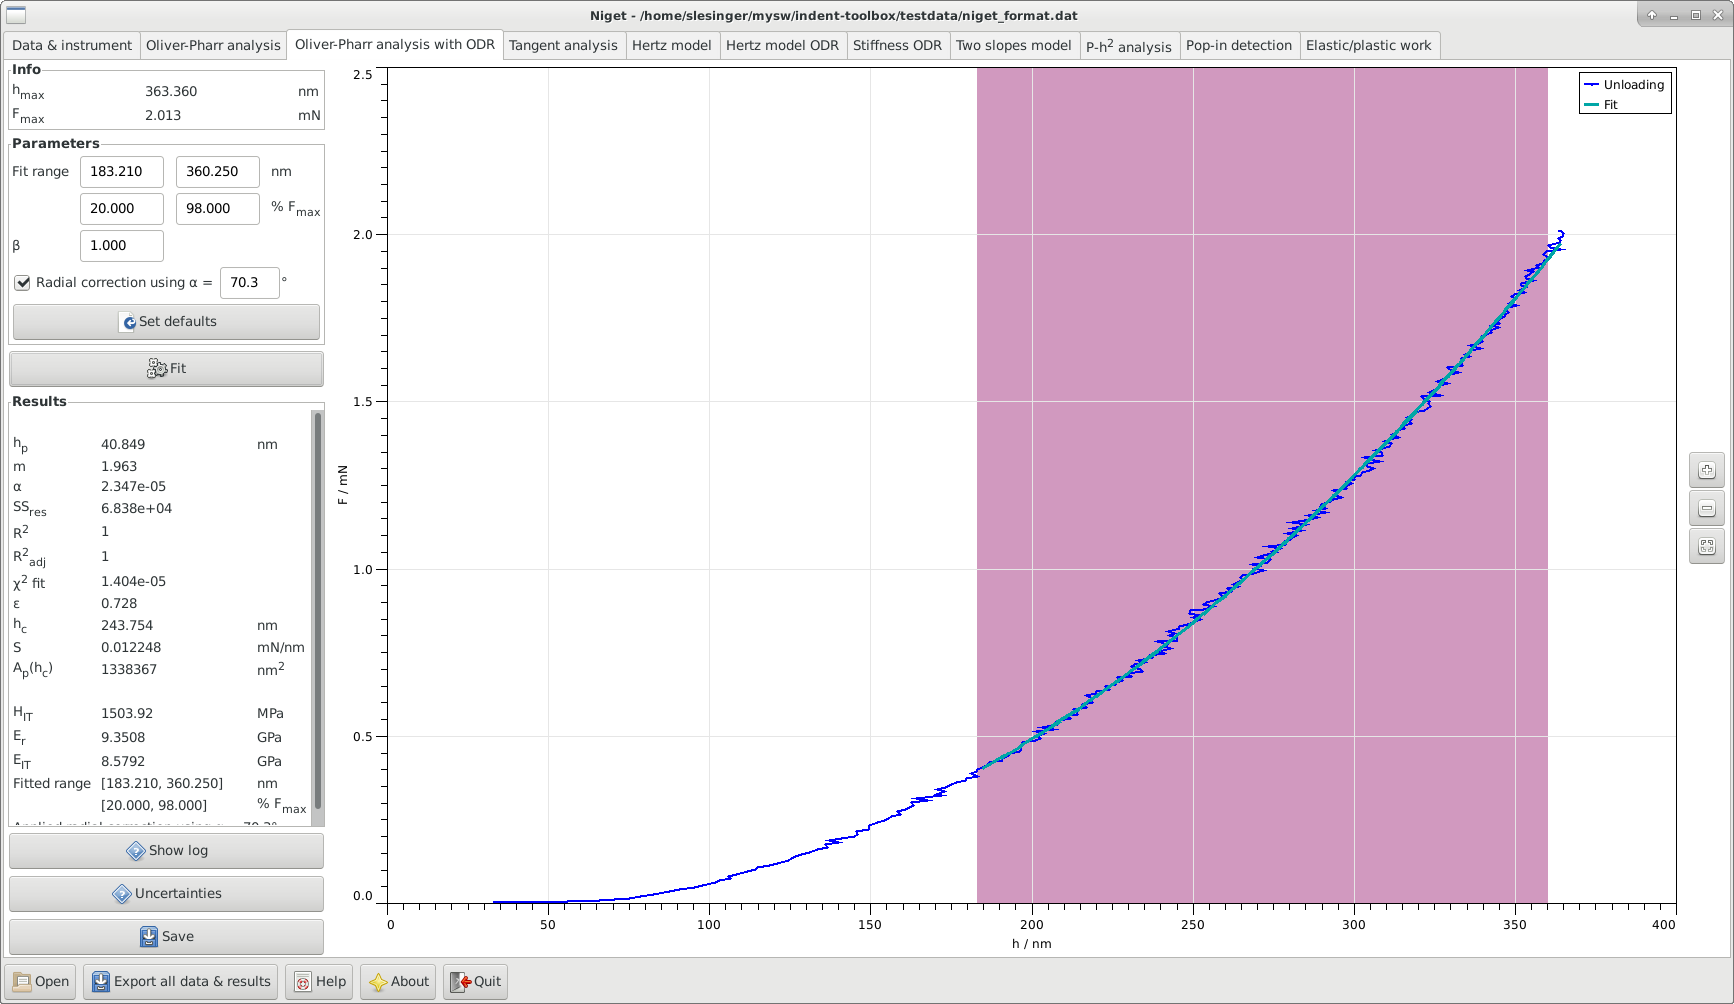
\includegraphics[width=\textwidth]{images/screen-op-odr}
  \caption{Oliver-Pharr analysis using orthogonal data regression}
\end{figure}

\subsection{Window}
The window consists of several blocks:
\begin{itemize}
 \item \emph{Info} displays the maximum depth and force during the indentation
 \item \emph{Parameters} shows the selected range in nm and in \% of the maximum force, the correction $\beta$, and the radial correction. 
        \begin{itemize}
          \item[-] The fitting range can be selected either using the mouse or typing in the range entries. The range can be defined either in nm or in percent of the maximum force. 
                   It is often recommended to use the range 40--98 \% F$_\mathrm{max}$ for the fit, see section \ref{opodr_calc}.  
          \item[-] The parameter $\beta$ accounts for any deviations from the axisymmetric case and is used in the calculation of the reduced modulus in equation \eqref{eq:Er}. 
                   Currently, the default value is no correction $\beta = 1.0$. The value supplied by the user is saved in the settings and can be reset to its default value.
                 \item[-] Optional radial correction of calculated hardness and modulus values according to ISO 14577-1:2015. The angle $\alpha$ denotes the cone-equivalent angle between the tip side and axis. For a Berkovich tip, $\alpha = 70.3^\circ$.
                   \item \emph{Set defaults} button resets the fitting range, the beta value, and radial correction settings according to recommendations provided in ISO 14577-1.
          \end{itemize}
 \item \emph{Fit} button, see section \ref{opodr_calc} for details of the calculation.
 \item \emph{Results} displays all results in the following order: the residual depth $\hp$, the power $m$ of the power law function, the parameter $\varepsilon$, 
       the contact depth  $\hc$, the slope $S$, the contact area $\Ap(\hc)$, the indentation hardness $H_{IT}$, the contact modulus $E_r$, the indentation modulus $E_{IT}$ and the ranges used for the fitting procedure.
       The variables are described in detail in section \ref{opodr_calc}. If the fittings procedure failed a warning is shown.
 \item \emph{Uncertainties} show the uncertainty analysis window, see section \ref{opodr_unc}.
 \item \emph{Show log} Show the report about the fitting procedure in a separate window.  The reports are saved to files \emph{fit.log.op.err} and \emph{fit.log.op.rpt}. 
 \item \emph{Save} save parameters and results to given file. 
 \item \emph{Graph} display the unloading curve and the fitted curves. Stepwise zooming/unzooming can be performed by selecting a range with the mouse and pressing the \emph{Zoom}/ \emph{Unzoom} buttons. The graph is restored to its original size by the \emph{Restore} button.
\end{itemize}

\subsection{Procedure} \label{opodr_calc}
This is a slight modification of the standard Oliver Pharr method described in section \ref{op_calc} using a better fitting procedure. 
\begin{enumerate} 
 \item 
 Fit the upper part of the unloading curve with a power law function
$$
F = \alpha (h - \hp)^m.
$$
using orthogonal least squares as implemented in the package ODRPACK95 \cite{odrpack95}. The range should be approx. 40--98 \% F$_\mathrm{max}$. All three parameters are fitted.
\item  Same as steps 3--4 in \ref{op_calc}.
\item If the radial correction is on, the hardness and reduced modulus are found by iterating the following relations
\begin{eqnarray}
 H^n &=& H^0 \left(1+K \frac{H^{n-1}}{E_{IT}^{n-1}}\right)^2 \\
 E_r^n &=& E_r^0 \left(1+K \frac{H^{n-1}}{E_{IT}^{n-1}}\right)
\end{eqnarray}
where $H^0$ and $E_r^0$ are the initial estimates obtained from step 4 in section \ref{op_calc}. The iteration limit is set to a relative difference $0.5 \cdot 10^{-4}$
Young's modulus is updated in each step according to \eqref{eq:Eit} and $K$ is the radial correction factor computed from Poisson's ratio and the angle between tip sides and axis $\alpha$
\begin{equation}
 K = \frac{1-2 \nu}{2(1+\nu)} \sin \alpha.
\end{equation}
The area function is corrected with the final values of hardness and modulus as 
\begin{equation}
 A = A^0 \left(1+K \frac{H}{E_{IT}}\right)^2.
\end{equation}




\end{enumerate}


% Tangent method
%--------------- Tangent method ---------

\section{Tangent method} \label{tg}
The method is based on the linear model as described in \cite{doerner1986}. It is recommended only for use with highly plastic materials where the depth of elastic
recovery is less than 10 \% of max.

\begin{figure}[ht]
  \centering
  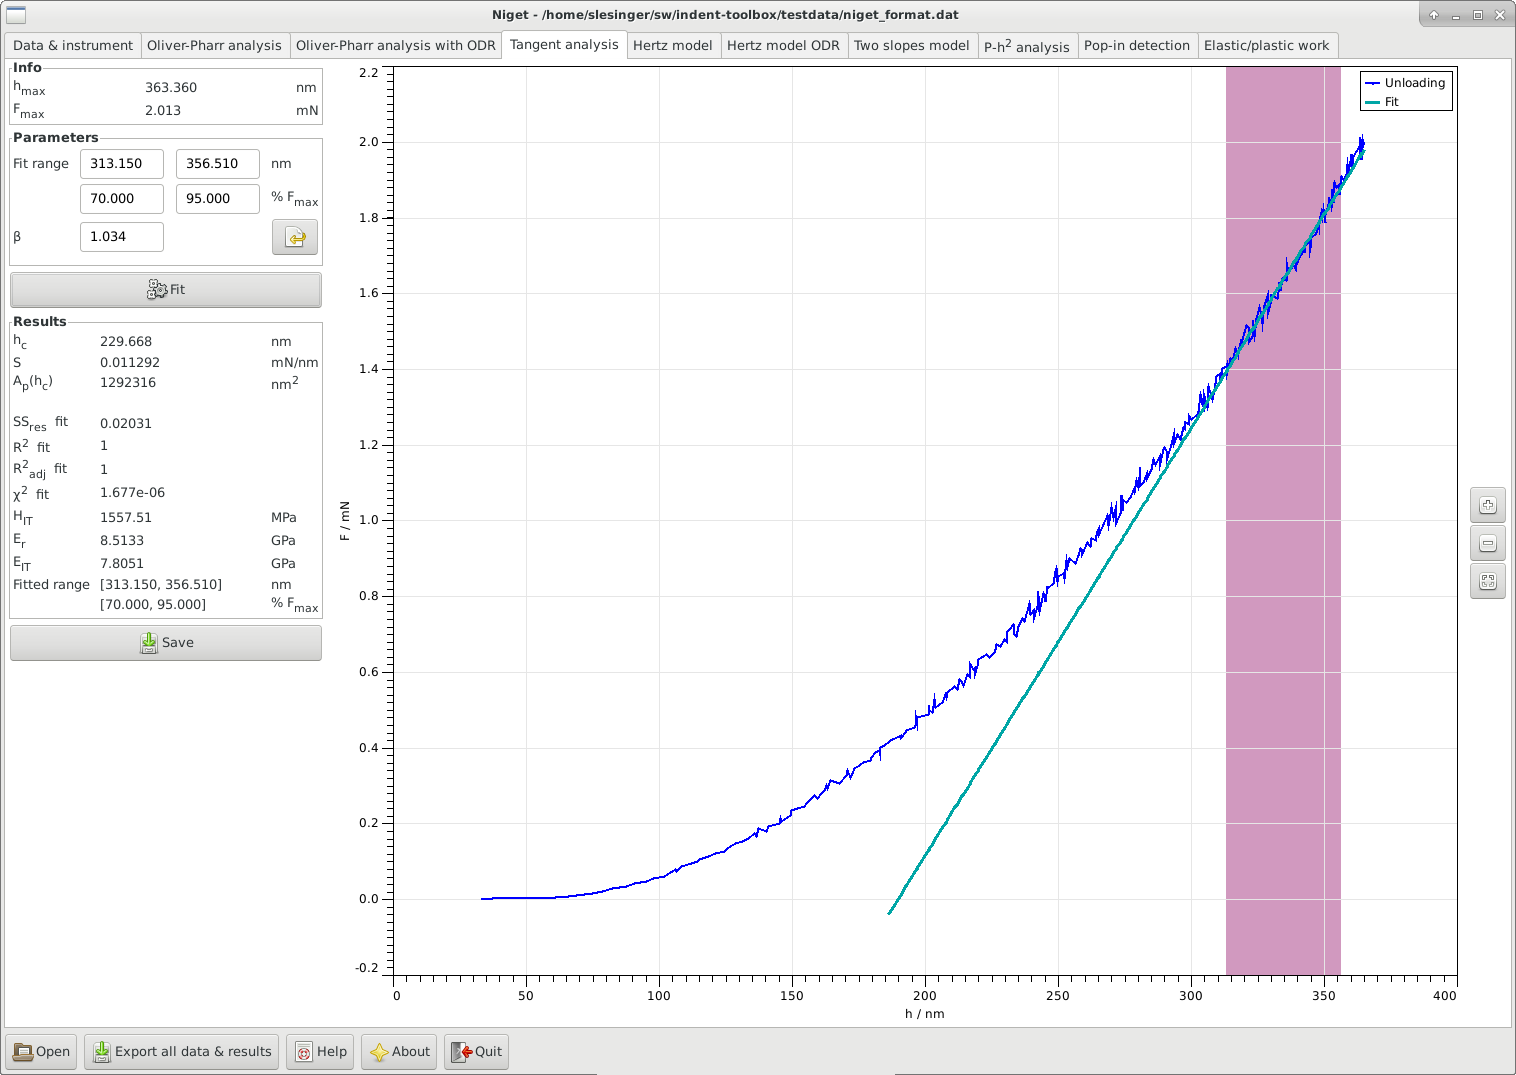
\includegraphics[width=\textwidth]{images/screen-tangent}
  \caption{Tangent method analysis}
\end{figure}


\subsection{Window}
The window consists of several blocks:
\begin{itemize}
 \item \emph{Info} displays the maximum depth and force during the indentation
 \item \emph{Parameters} shows the selected range in nm and in \% of the maximum force, and the correction $\beta$. 
        \begin{itemize}
          \item[-] The fitting range can be selected either using the mouse or typing in the range entries. The range can be defined either in nm or in percent of the maximum force. 
                   It is often recommended to use the range 70--95 \% F$_\mathrm{max}$ for the fit, see section \ref{tg_calc}.  
          \item[-] The parameter $\beta$ accounts for any deviations from the axisymmetric case and is used in the calculation of the reduced modulus in equation \eqref{eq:Er}. 
                   Currently, the default value is the value for three-sided pyramides $\beta = 1.034$. The value supplied by the user is saved in the settings and can be reset to its default value.
        \end{itemize}
 \item \emph{Fit} button, see section \ref{tg_calc} for details of the calculation.
 \item \emph{Results} displays all results in the following order: the contact depth  $\hc$, the slope $S$, the contact area $\Ap(\hc)$, the indentation hardness $H_{IT}$, the contact modulus $E_r$, the indentation modulus $E_{IT}$ and the ranges used for the fitting procedure.
       The variables are described in detail in section \ref{tg_calc}.
 %\item \emph{Uncertainties} show the uncertainty analysis window, see section \ref{tg_unc}.
 \item \emph{Save} save parameters and results to given file. 
 \item \emph{Graph} display the unloading curve and the fitted curves. Stepwise zooming/unzooming can be performed by selecting a range with the mouse and pressing the \emph{Zoom}/ \emph{Unzoom} buttons. The graph is restored to its original size by the \emph{Restore} button.
\end{itemize}

\subsection{Procedure} \label{tg_calc}
The tangent method uses a different approach to determine the slope of the unloading curve at its maximum depth than the Oliver Pharr method.
\begin{enumerate}
 \item Fit the uppermost part of the unloading curve with a straight line using a Deming fit with $\delta = \sigma_F^2/\sigma_h^2$, see section \ref{tls},
 $$
 F = S h + q,
 $$
 using total least squares. The range should be approx. 70--95 \% F$_\mathrm{max}$.
 \item Set $\varepsilon = 0.75$ and calculate the contact depth as
  \begin{equation} \label{eq:hc_tg}
   \hc = \hmax - \varepsilon \Fmax/S.
  \end{equation}

 \item Same as step 4 in \ref{op_calc}.
\end{enumerate}



% simple Hertz method
%-------------- Hertz -----------------------
\section{Hertz method} \label{hertz}
The Hertz method is the application of the Hertzian model of elastic contact to the initial stage of the loading curve \cite{Hertz}. 
It can be used either to estimate the modulus if the tip radius is known or vice versa, depending what information is available.

\begin{figure}[h]
  \centering
  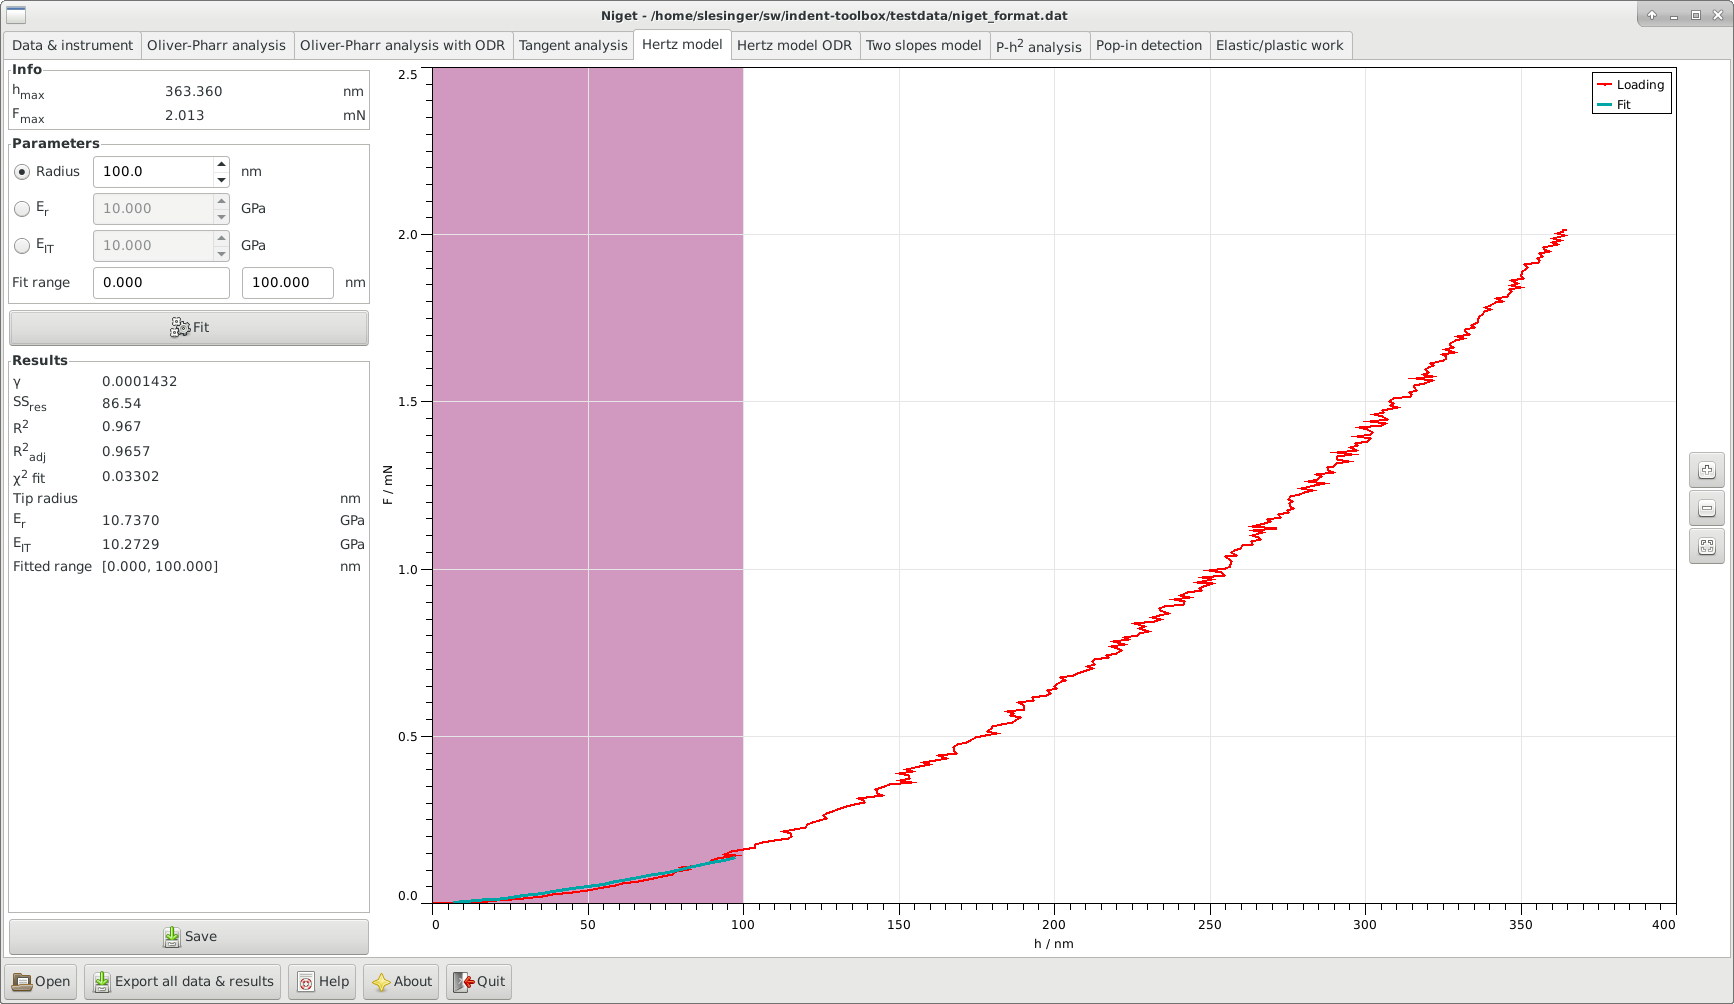
\includegraphics[width=\textwidth]{images/screen-hertz}
  \caption{Hertzian model analysis}
\end{figure}

\subsection{Window}
The window consists of several blocks:
\begin{itemize}
 \item \emph{Info} displays the maximum depth and force during the indentation
 \item \emph{Parameters} shows the selected range in nm. 
        \begin{itemize}
           \item[-] The input variable can be chosen to be either the tip radius, the reduced modulus or the indentation modulus and its value should be set accordingly.
           \item[-] The fitting range can be selected either using the mouse or typing in the range entries. The range must be chosen so that the behavior remains elastic and the fit adequate.
        \end{itemize}
 \item \emph{Fit} button, see section \ref{hertz_calc} for details of the calculation.
 \item \emph{Results} displays the results and the ranges used for the fitting procedure. 
       The variables are described in detail in section \ref{hertz_calc}.
% \item \emph{Uncertainties} show the uncertainty analysis window, see section \ref{hertz_unc}.
 \item \emph{Save} save parameters and results to given file. 
 \item \emph{Graph} display the unloading curve and the fitted curves.  Stepwise zooming/unzooming can be performed by selecting a range with the mouse and pressing the \emph{Zoom}/ \emph{Unzoom} buttons. The graph is restored to its original size by the \emph{Restore} button.
\end{itemize}

\subsection{Procedure} \label{hertz_calc}
\begin{enumerate} 
 \item 
The Hertzian model predicts for the contact between sphere and halfspace the following shape of the loading curve
\begin{equation} \label{eq:hertzfit}
F = a h^{3/2},  
\end{equation}
with 
\begin{equation}
a = \frac43 \Er \sqrt{R}.
\end{equation}
This is fitted using ordinary least squares with an additional intercept possible, see section \ref{ls:fit32}.
\item
If the tip radius is given, the contact modulus is calculated as 
\begin{equation}
\Er = \frac34 \frac{a}{\sqrt{R}}.
\end{equation}
For a comparison with Young's modulus found in literature the indentation modulus $E_{IT}$ \eqref{eq:Eit} is useful

\item
If the reduced modulus is given, the tip radius is calculated as
\begin{equation}
R =  \left(\frac34 \frac{a}{\Er}\right)^2
\end{equation}
\item
If the indentation reduced modulus is given, the material parameters $\nu$, $\nui$ and $\Ei$ are used to convert it to the reduced modulus
\begin{equation}
\Er=\left(\frac{1-\nui^2}{\Ei}+\frac{1-\nu^2}{\Eit}\right)^{-1}.
\end{equation}
from which the tip radius can be calculated as in the previous step.
\end{enumerate}


% Hertz ODR 
%---------------------------------- Hertz ODR -----------------------------
\section{Hertz method with ODR} \label{hertz_odr}
This is a modification of the Hertz method explained in section \ref{hertz} and uses orthogonal distance regression. 
The loading curve is fitted with a more general power function but the relationship between the proportionality coefficient and the radius and modulus is assumed to stay the same.
If the resulting power differs from the theoretical value 1.5, this is an indicator that the Hertzian model is not adequate. The results for radius or modulus in this case do not make any physical sense.\\
This method is shown unless the software was compiled without Fortran support.  \\

\begin{figure}[ht]
  \centering
  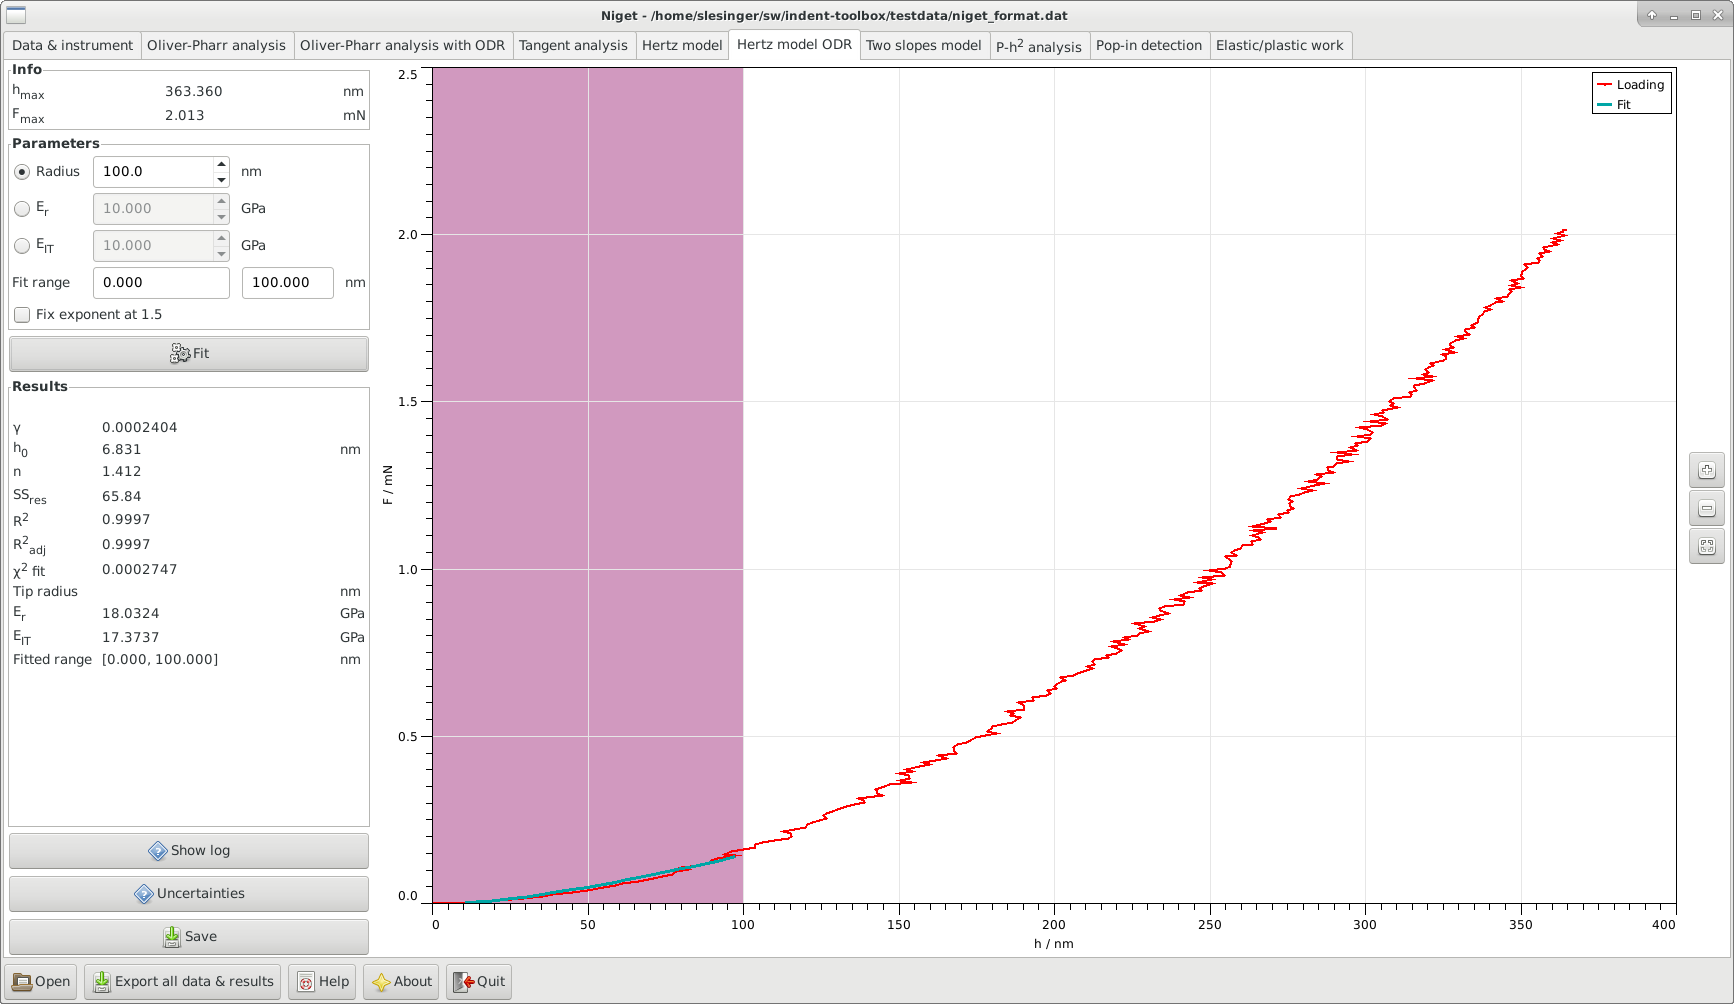
\includegraphics[width=\textwidth]{images/screen-hertz-odr}
  \caption{Hertzian model with ODR analysis}
\end{figure}

\subsection{Window}
The window consists of several blocks:
\begin{itemize}
 \item \emph{Info} displays the maximum depth and force during the indentation
 \item \emph{Parameters} shows the selected range in nm. 
        \begin{itemize}
           \item[-] The input variable can be chosen to be either the tip radius, the reduced modulus or the indentation modulus and its value should be set accordingly.
           \item[-] The fitting range can be selected either using the mouse or typing in the range entries. The range must be chosen so that the behavior remains elastic and the fit adequate.
           \item[-] Check box, whether or not the exponent should be fitted or fixed at the value 1.5, see \ref{hertz_odr_calc}.
        \end{itemize}
 \item \emph{Fit} button, see section \ref{hertz_odr_calc} for details of the calculation.
 \item \emph{Results} displays the results and the ranges used for the fitting procedure. 
       The variables are described in detail in section \ref{hertz_odr_calc}.
 \item \emph{Show log} Show the report about the fitting procedure in a separate window.  The reports are saved to files \emph{fit.log.hz.err} and \emph{fit.log.hz.rpt}.
 \item \emph{Uncertainties} show the uncertainty analysis window, see section \ref{hertz_odr_unc}.
 \item \emph{Save} save parameters and results to given file. 
 \item \emph{Graph} display the unloading curve and the fitted curves.  Stepwise zooming/unzooming can be performed by selecting a range with the mouse and pressing the \emph{Zoom}/ \emph{Unzoom} buttons. The graph is restored to its original size by the \emph{Restore} button.
\end{itemize}

\subsection{Procedure} \label{hertz_odr_calc}
\begin{enumerate} 
 \item 
The Hertzian model \eqref{eq:hertzfit} is fitted with a more general function 
\begin{equation} \label{eq:hertzodrfit}
F = \gamma  (h - h_0)^{n},  
\end{equation}
using orthogonal least squares implemented in ODRPACK. 
The power $n$ can be fixed at the theoretical value 1.5.
\item  
Further steps are the same as steps 2--4 in section \ref{hertz_calc} with $\gamma$ used instead of $a$. 
\end{enumerate}


% Stiffness ODR
%-------- Stiffness method ---------------
\section{Stiffness method}
This module allows the determination of the stiffness of an object by fitting both loading and unloading curve with a straight line. 
This method is shown unless the software was compiled without Fortran support.  \\

\begin{figure}[ht]
  \centering
  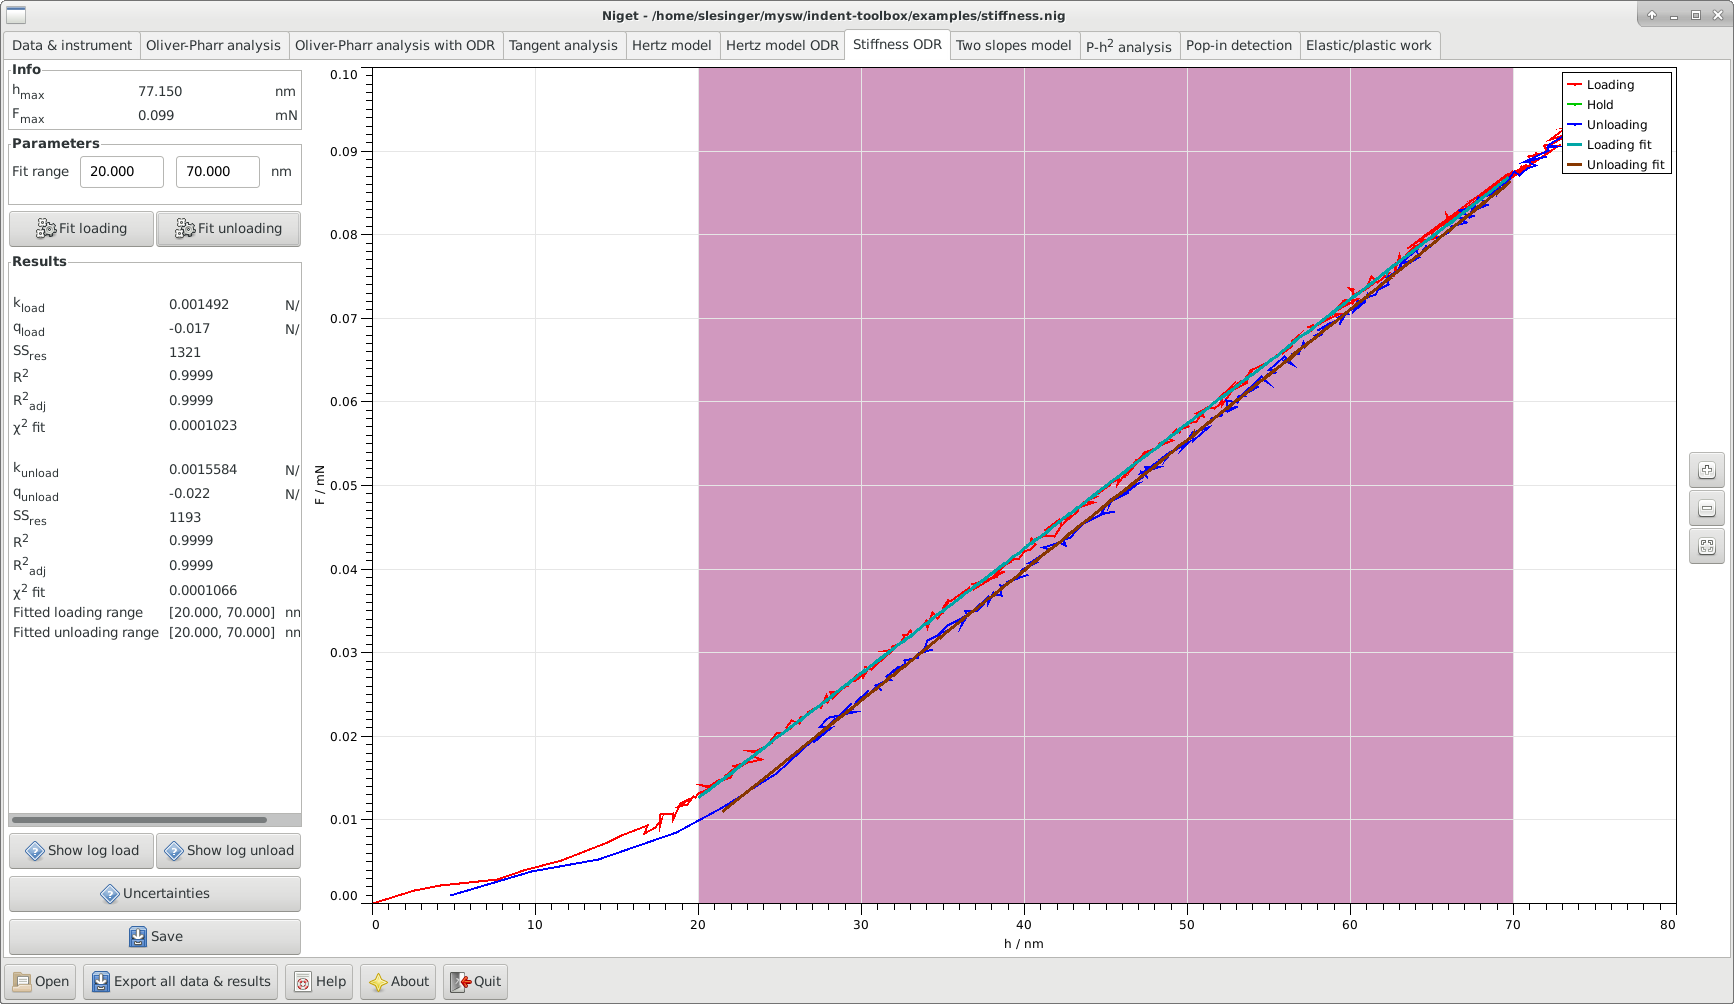
\includegraphics[width=\textwidth]{images/screen-stiffness}
  \caption{Stiffness analysis using orthogonal data regression}
\end{figure}

\subsection{Window}
The window consists of several blocks:
\begin{itemize}
 \item \emph{Info} displays the maximum depth and force during the indentation
 \item \emph{Parameters} shows the selected range in nm and in \% of the maximum force, and the correction $\beta$. 
        \begin{itemize}
          \item[-] The fitting range can be selected either using the mouse or typing in the range entries.   
        \end{itemize}
 \item \emph{Fit} buttons for indepedent fitting of the loading and unloading curves, see section \ref{stiffness_calc} for details of the calculation.
 \item \emph{Results} displays all results in the following order: 
       the slope of the loading curve $\kl$, the offset of the loading curve $\ql$, 
       the residual sum of squares of the corresponding fit and the goodness of fit parameters,
       the slope of the unloading curve $\ku$, the offset of the loading curve $\qu$,
        the residual sum of squares of the corresponding fit and the goodness of fit parameters
       and the ranges used for the fitting procedures.
       Warnings are displayed if the fittings procedures failed.
 \item \emph{Uncertainties} show the uncertainty analysis window, see section \ref{stiffness_unc}.
 \item \emph{Show log load} Show the report about the fitting procedure of the loading curve in a separate window.  The reports are saved to files \emph{fit.log.stiff.load.err} and \emph{fit.log.stiff.load.rpt}. 
 \item \emph{Show log unload} Show the report about the fitting procedure of the unloading curve in a separate window.  The reports are saved to files \emph{fit.log.stiff.unload.err} and \\ \emph{fit.log.stiff.unload.rpt}. 
 \item \emph{Save} save parameters and results to given file. 
 \item \emph{Graph} display the unloading curve and the fitted curves. Stepwise zooming/unzooming can be performed by selecting a range with the mouse and pressing the \emph{Zoom}/ \emph{Unzoom} buttons. The graph is restored to its original size by the \emph{Restore} button.
\end{itemize}

\subsection{Procedure} \label{stiffness_calc}
The stiffness analysis simply fits both loading and unloading curve with straight lines. 
\begin{enumerate} 
 \item 
 Fit the loading curve with a straight line 
$$
F = \kl h + \ql
$$
using orthogonal least squares as implemented in the package ODRPACK95 \cite{odrpack95}.
\item
Fit the unloading curve with a straight line 
$$
F = \ku h + \qu
$$
using orthogonal least squares as implemented in the package ODRPACK95 \cite{odrpack95}. 

\end{enumerate}




% Two slopes method
% ------------ Two slopes method --------------------
\section{Two slopes method}
For a description of the two slopes method see \cite{Oliver}. \\ 
This method is shown unless the software was compiled without Fortran support.  \\

\begin{figure}[ht]
  \centering
  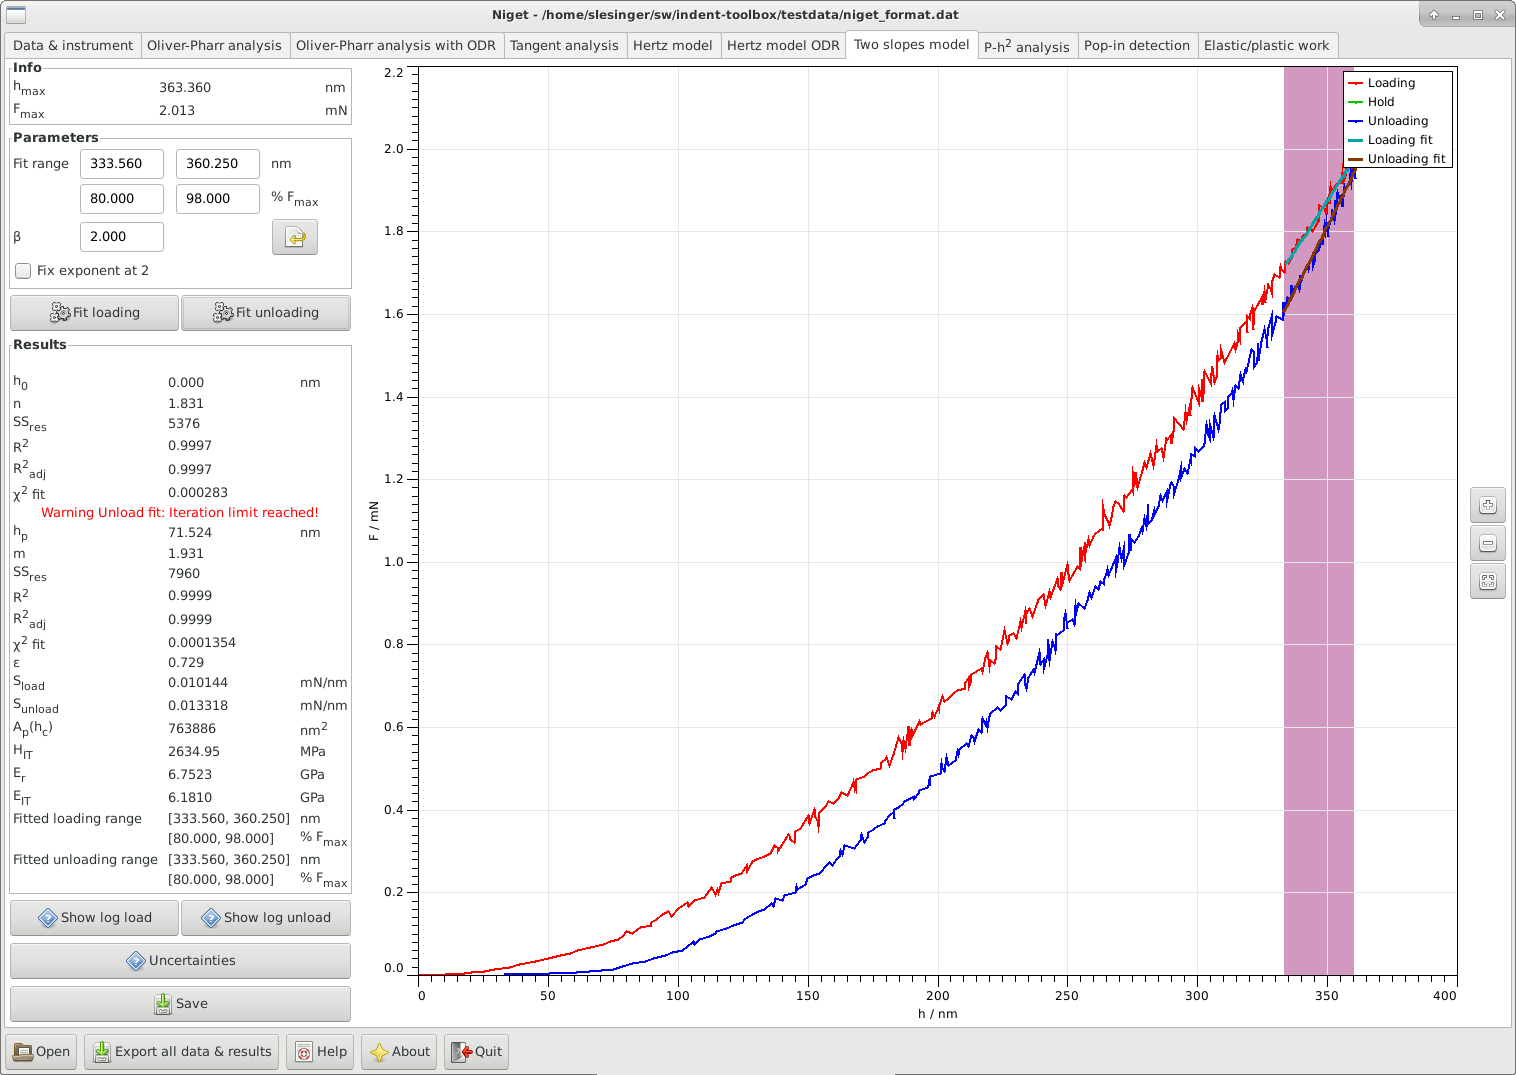
\includegraphics[width=\textwidth]{images/screen-twoslopes}
  \caption{Two slopes analysis using orthogonal data regression}
\end{figure}

\subsection{Window}
The window consists of several blocks:
\begin{itemize}
 \item \emph{Info} displays the maximum depth and force during the indentation
 \item \emph{Parameters} shows the selected range in nm and in \% of the maximum force, and the correction $\beta$. 
        \begin{itemize}
          \item[-] The fitting range can be selected either using the mouse or typing in the range entries. The range can be defined either in nm or in percent of the maximum force. 
                   It is often recommended to use the range 80--98 \% F$_\mathrm{max}$ for the fit, see section \ref{slopes_calc}.  
          \item[-] The parameter $\beta$ accounts for any deviations from the axisymmetric case and is used in the calculation of the reduced modulus in equation \eqref{eq:Er}. 
                   Currently, the default value is no correction $\beta = 1.0$. The value supplied by the user is saved in the settings and can be reset to its default value.
          \item[-] Check box, whether or not the exponent of the loading curve should be fitted or fixed at the theoretical value 2, see \ref{slopes_calc}.
          \end{itemize}
 \item \emph{Fit} buttons for indepedent fitting of the loading and unloading curves, see section \ref{slopes_calc} for details of the calculation.
 \item \emph{Results} displays all results in the following order: 
       the auxiliary depth parameter $h_0$, the power $n$ of the power law loading function, 
       the residual depth $\hp$, the power $m$ of the power law unloading function, the parameter $\varepsilon$, 
       the loading slope $\Sload$, the unloadingslope $\Sunload$, 
       the contact area $\Ap(\hc)$, the indentation hardness $H_{IT}$, the contact modulus $E_r$, the indentation modulus $E_{IT}$ and the ranges used for the fitting procedures.
       The variables are described in detail in section \ref{slopes_calc}. Warnings are displayed if the fittings procedures failed.
 \item \emph{Uncertainties} show the uncertainty analysis window, see section \ref{slopes_unc}.
 \item \emph{Show log load} Show the report about the fitting procedure of the loading curve in a separate window.  The reports are saved to files \emph{fit.log.slopes.load.err} and \emph{fit.log.slopes.load.rpt}. 
 \item \emph{Show log unload} Show the report about the fitting procedure of the unloading curve in a separate window.  The reports are saved to files \emph{fit.log.slopes.unload.err} and \\ \emph{fit.log.slopes.unload.rpt}. 
 \item \emph{Save} save parameters and results to given file. 
 \item \emph{Graph} display the unloading curve and the fitted curves. Stepwise zooming/unzooming can be performed by selecting a range with the mouse and pressing the \emph{Zoom}/ \emph{Unzoom} buttons. The graph is restored to its original size by the \emph{Restore} button.
\end{itemize}

\subsection{Procedure} \label{slopes_calc}
The two slopes method combines the standard Oliver Pharr method and the quadratic loading curve to avoid the need of the contact area.
\begin{enumerate} 
 \item 
 Fit the upper part of the loading curve with a power law function
$$
F = \gamma (h - h_0)^n.
$$
using orthogonal least squares as implemented in the package ODRPACK95 \cite{odrpack95}. The range should be approx. 85--98 \% F$_\mathrm{max}$. The exponent $n$ can be kept fixed at its theoretical value 2.
 \item 
 Fit the upper part of the unloading curve with a power law function
$$
F = \alpha (h - \hp)^m.
$$
using orthogonal least squares as implemented in the package ODRPACK95 \cite{odrpack95}. The range should be approx. 85--98 \% F$_\mathrm{max}$. All three parameters are fitted.
\item The auxiliary parameter $\varepsilon$ is calculated from the power $m$ as in \eqref{eq:eps}
\item The slopes at the maximum depth are calculated as
\begin{eqnarray} \label{eq:Stwo}
\Sload &=& n \frac{ \Fmax}{\hmax-h_0} \\
\Sunload &=& m \frac{ \Fmax}{\hmax-\hp} 
\end{eqnarray}
\item 
The contact area, indentation hardness and contact modulus are calculated as
\begin{eqnarray}
 \Ap(\hc) &=& C_0 \Fmax^2 \left( \frac{2 \Sunload -\beta \varepsilon \Sload}{\Sunload \Sload} \right)^2 \\
 \Hit &=& \frac1{C_0 \Fmax} \left( \frac{\Sunload \Sload}{2 \Sunload -\beta \varepsilon \Sload} \right)^2 \\
 \Er &=& \frac1{2 \beta \Fmax}  \sqrt{\frac \pi{C_0}} \frac{\Sunload^2 \Sload}{2 \Sunload -\beta \varepsilon \Sload}
\end{eqnarray}
with $C_0$ the coefficient of the $h^2$ term in the area calibration function and $\beta$ a geometric correction term. Currently, we use $\beta = 1$.
\item
The indentation modulus can be calculated from \eqref{eq:Eit}

\end{enumerate}



%  F/h2  
% ------------ F/h2  ------
\section{F-h$^2$ analysis}
The analysis of $F$ vs $h^2$  follows \cite{mcgurk1999,Malzbender200172,Malzbender2000265}.

\begin{figure}[h]
  \centering
  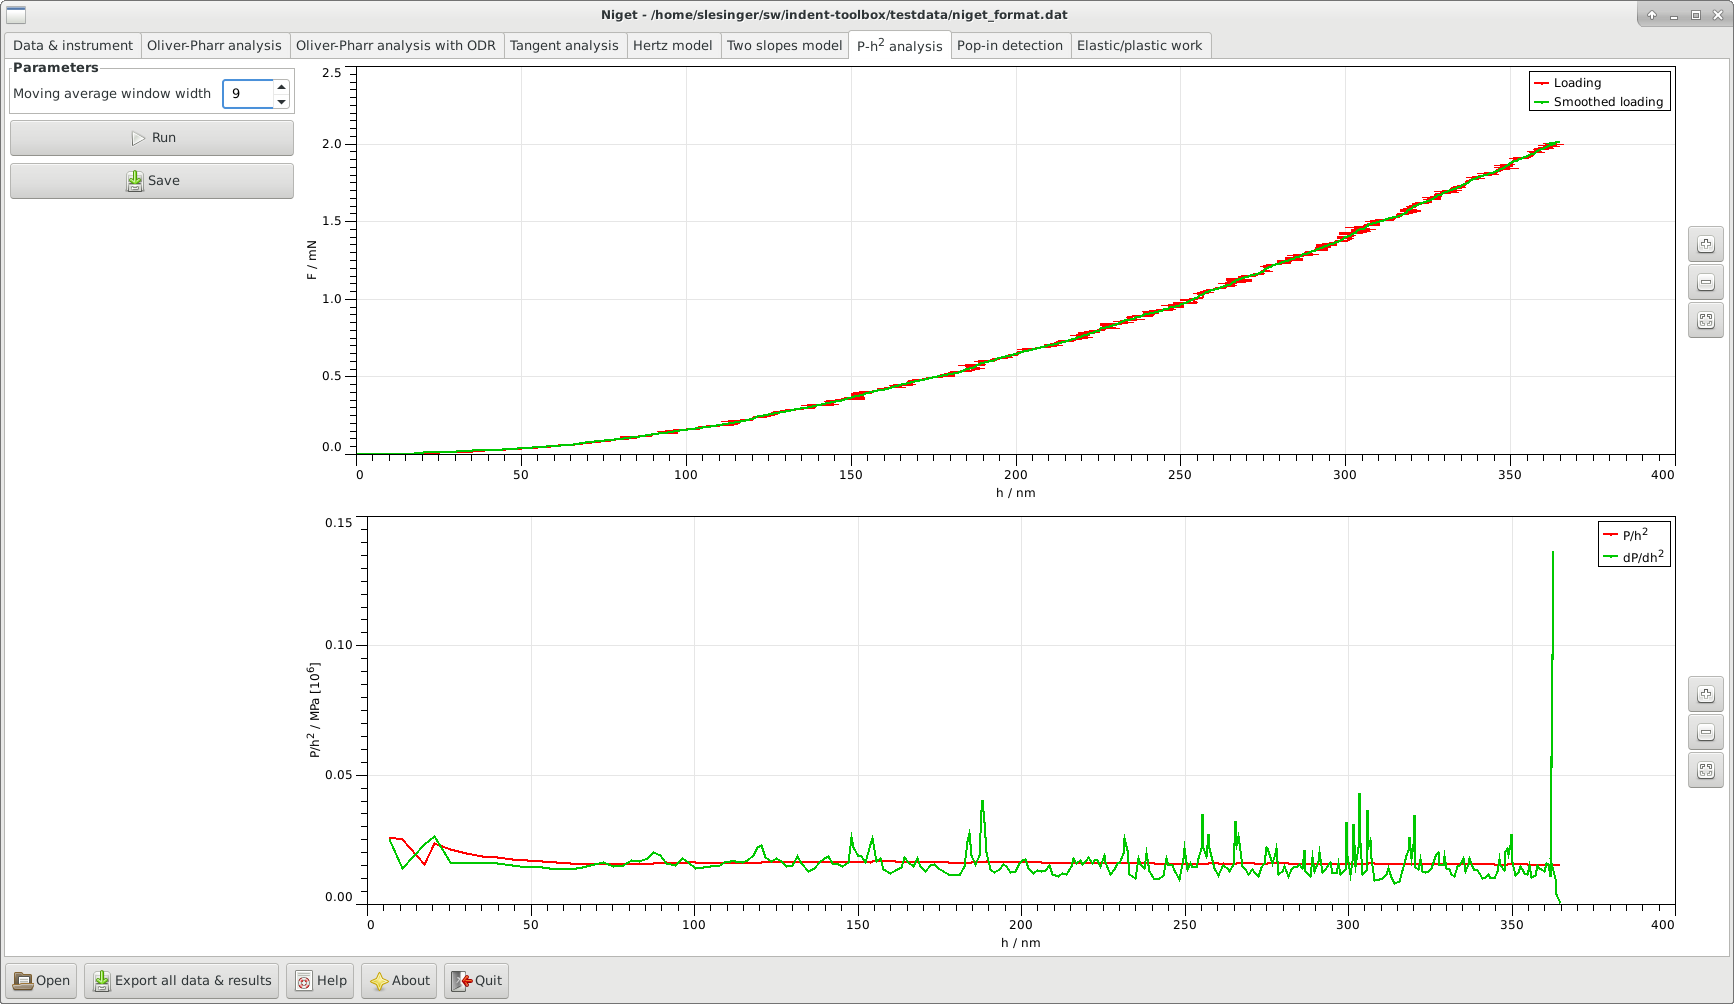
\includegraphics[width=\textwidth]{images/screen-ph2}
  \caption{$F$ vs $h^2$ analysis}
\end{figure}

\subsection{Window}
The window consists of several blocks:
\begin{itemize}
 \item \emph{Parameters} allows the user to set the width of the moving average window. The value~1 corresponds to no smoothing. This value is saved in settings. 
 \item \emph{Run}  perform calculation and display curve, see section \ref{Ph2_calc}. 
 \item \emph{Save} save parameters and results to given file. 
 \item \emph{Graph}  
    \begin{itemize} \item[] Top: display the loading curve and the smoothed curve. 
		    \item[] Bottom: display the $F/h^2$ and the $\mathrm{d}F/\mathrm{d} h^2$ curves.     
    \end{itemize}
 Stepwise zooming/unzooming can be performed by selecting a range with the mouse and pressing the \emph{Zoom}/ \emph{Unzoom} buttons. 
		     The graph is restored to its original size by the \emph{Restore} button. Zooming in the two graphs is independent.
  \end{itemize}

\subsection{Procedure}\label{Ph2_calc}
\begin{enumerate}
 \item 
We use a moving average with a fixed width and constant weight. This means we substitute a value with its average with $s$ values to the left and to the right, $w = 2s + 1$ 
$$
\hat{x} _i = \frac1w \sum_{j = -s}^{s} x_{i+j}.
$$
The value $w = 1$ corresponds to the original data. There is only one moving average type defined for both depth and load.
Increasing the value of $w$ noise becomes less influential but important small effects can get lost as well. 
Therefore, the value should not be too large, below 11 is recommended.

\item The ratio $F/h^2$ is calculated for for each data pair $(\hat{h},\hat{F})$ of the (smoothed) loading curve and plotted as a function of the (smoothed) depth $\hat{h}$.
\item The derivative $\mathrm{d}F/\mathrm{d}h^2$ is calculated for for each data pair $(\hat{h},\hat{F})$ of the (smoothed) loading curve and plotted as a function of the (smoothed) depth $\hat{h}$.
The derivative is done numerically as the ratio of the derivatives of $F$ and $h$ with respect to the (time)step or index $i$ 
$$
\frac{\mathrm{d}F}{\mathrm{d} h^2} = \frac{\mathrm{d}F}{\mathrm{d}i} \left(  \frac{\mathrm{d}h^2}{\mathrm{d}i}\right)^{-1}.
$$
The numerical derivatives are calculated using the three-point formula for equally spaced data.
\end{enumerate}



% pop-in
% -------------- brute force popin detection ------

\section{Pop-in detection}
The pop-in effect is a reaction of the crystalline structure to load. Defects of the crystalline structure occur during loading, these then reveal themselves as discontinuous jumps in the depth at constant
load. The critical load values are characteristic for the given orientation of the given material and can be compared to theoretical predictions based on the knowledge of the crystal lattice.

\begin{figure}[ht]
  \centering
  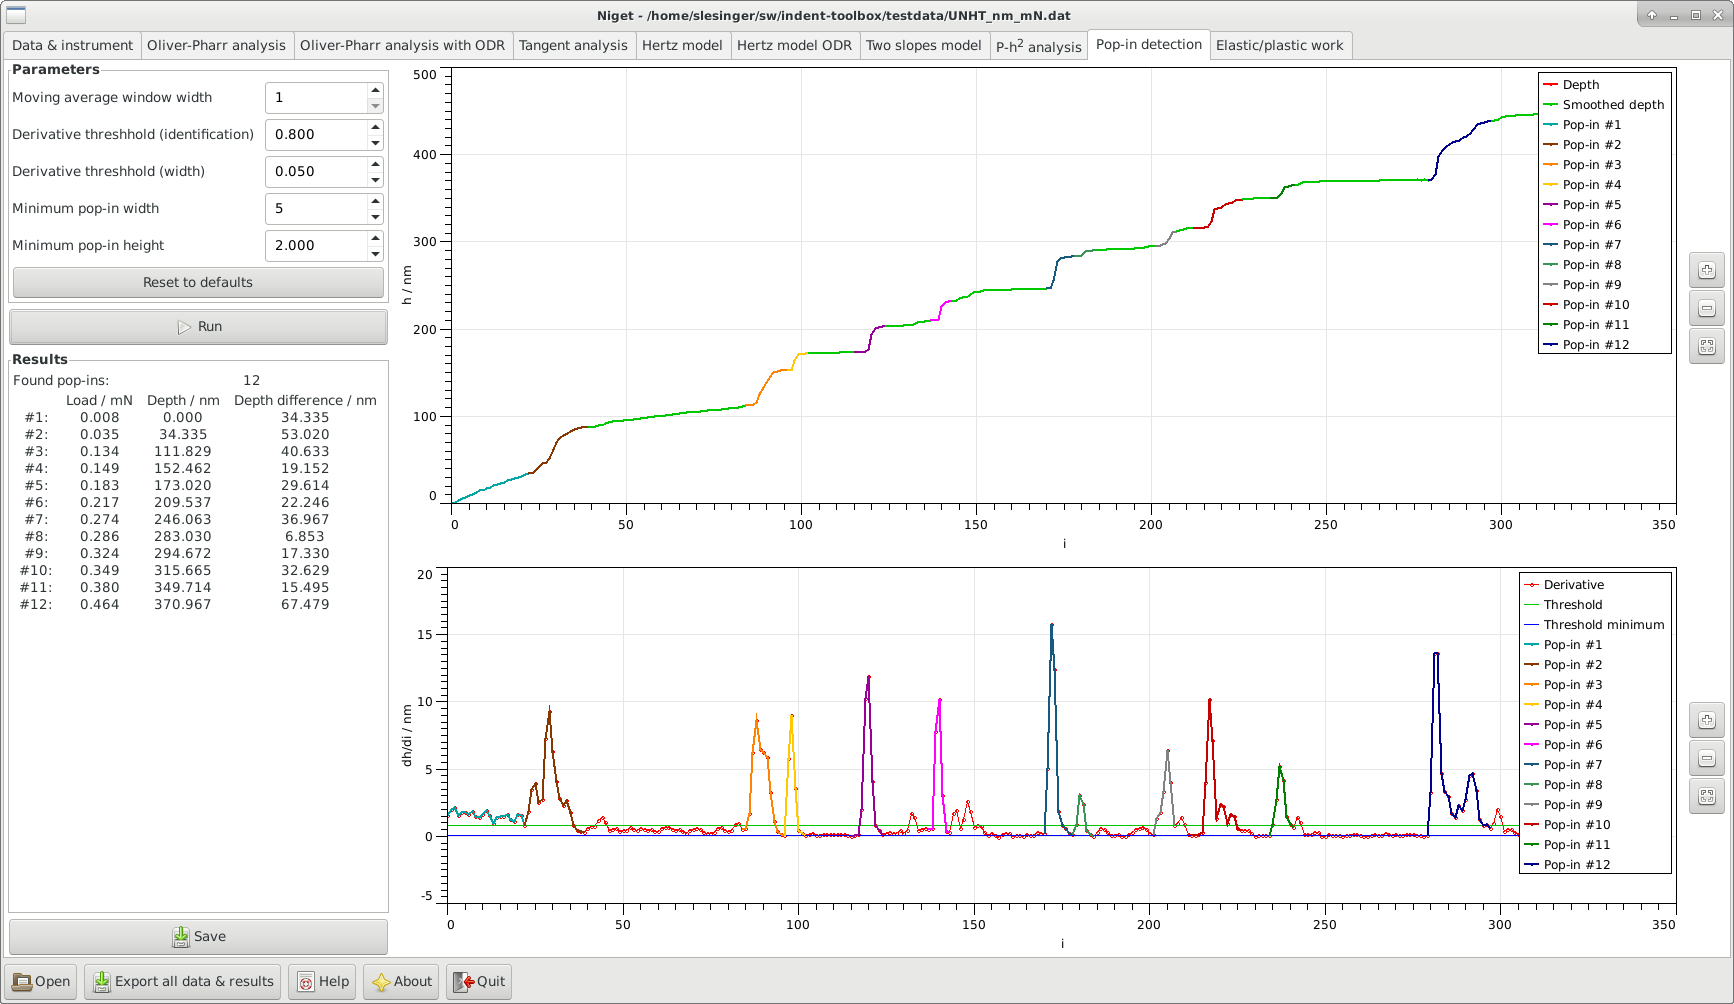
\includegraphics[width=\textwidth]{images/screen-popins}
  \caption{Pop-in detection}
\end{figure}

\subsection{Window}
The window consists of several blocks:
\begin{itemize}
 \item \emph{Info} displays the maximum depth and force during the indentation
 \item \emph{Parameters} allows the user to set the following parameters and the selected range in nm. 
        \begin{itemize}
          \item[-] \emph{Moving average window width} the width of the moving average window. The value 1 corresponds to no smoothing.
          \item[-] \emph{Derivative threshold for pop-in detection} the minimum derivative to identify the point as a pop-in.
          \item[-] \emph{Derivative threshold for pop-in width} determines how far to extend the pop-in once it was identified.
          \item[-] \emph{Minimum pop-in width} minimum number of datapoints needed for a pop-in.
          \item[-] \emph{Minimum pop-in height} (in nm) minimum jump in height needed for a pop-in.
        \end{itemize}
        These values are saved in settings. Default values are provided, but most likely the user will have to find proper values for each curve. For a detailed description see \ref{popin_calc}
       
  \item \emph{Run}  perform calculation and display curve, see section \ref{popin_calc}. 
  \emph{Results} displays the found pop-in events, the load and depth at which they occurred and the jump in the depth associated with it, see section \ref{popin_calc}.
 \item \emph{Save} save parameters and results to given file. 
 \item \emph{Graph}  
    \begin{itemize} \item[] Top: display the loading curve and the smoothed curve. 
       \item[] Bottom: display the derivative of the depth with respect to the index (pseudo-time) together with the two derivative thresholds.
  \end{itemize}
  Identified pop-ins are shown in color. \\
  Stepwise zooming/unzooming can be performed by selecting a range with the mouse and pressing the \emph{Zoom}/ \emph{Unzoom} buttons. 
		     The graph is restored to its original size by the \emph{Restore} button. Zooming in the two graphs is independent.
\end{itemize}

\subsection{Procedure} \label{popin_calc}
There is no standardized procedure how to define pop-in events. We use here a brute force direct method. %\marginpar{vysvetlujici graf}
\begin{enumerate}
 \item 
We use a moving average with a fixed width and constant weight. This means we substitute a value with its average with $s$ values to the left and to the right, $w = 2s + 1$ 
$$
\hat{x} _i = \frac1w \sum_{j = -s}^{s} x_{i+j}.
$$
The value $w = 1$ corresponds to the original data. 
Increasing the value of $w$ noise becomes less influential but important small effects can get lost as well. 
Therefore, the value should not be too large, below 11 is recommended.
\item Calculate the derivative of the loading curve with respect to the index (pseudo-time). This is the numerical derivative (in this case threee point derivative with equal steps) 
$$
dx_i = \frac12(x_{i+1} - x_{i-1}), 
$$
where $h$ is the step in the data.
\item Find the indices $i$ for which $x_i$ is larger then the \emph{Derivative threshold for pop-in detection}
\item Group the indices found in the previous step into consecutive groups.
\item Enlarge each group of indices to the left and to the right to include all values larger than \emph{Derivative threshold for pop-in width}.
\item For each group, check that the difference between the leftmost and righmost index is at least \emph{Minimum pop-in width}.
\item For each group, check that the difference in depth between the leftmost and righmost point  is at least \emph{Minimum pop-in height}.
\item For each group, find the average load for the range between leftmost and rightmost, the depth at the leftmost point (beginning of the pop-in), the difference in height between the leftmost and rightmost point and the indices.
\end{enumerate}




% elastic-plastic work 
% ------- elastic plastic work -----------
\section{Elastic/plastic work} \label{work}
The elastic and plastic work can be calculated.

\begin{figure}[ht]
  \centering
  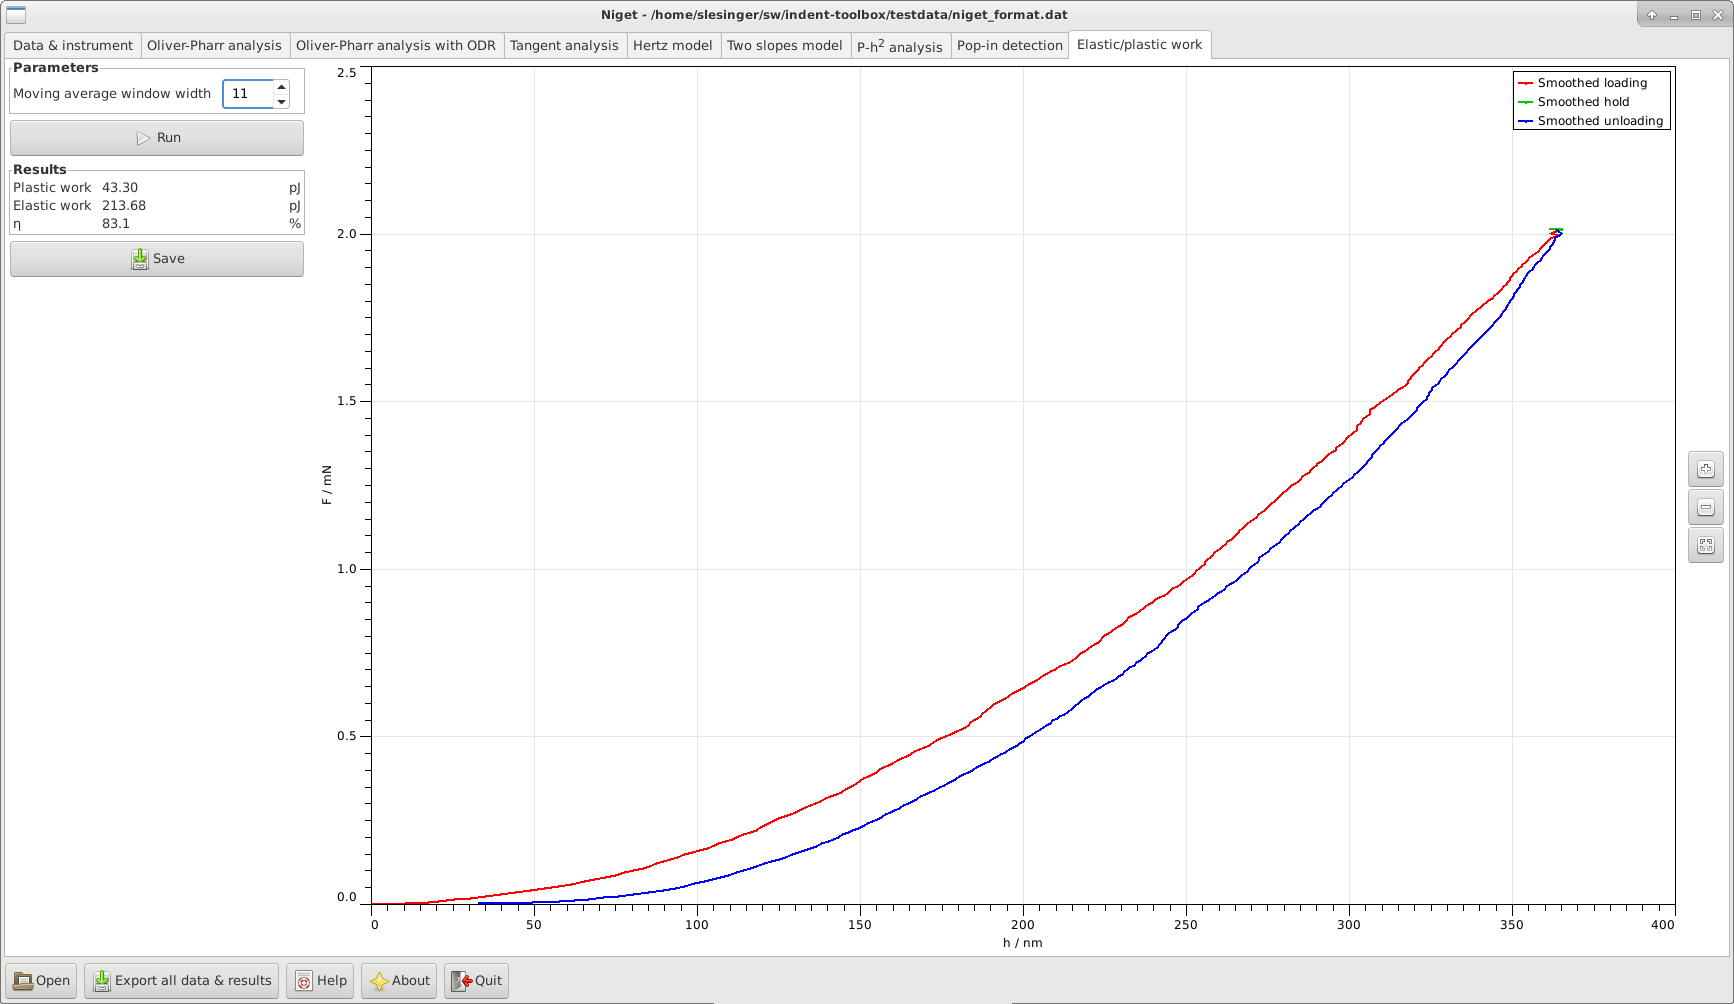
\includegraphics[width=\textwidth]{images/screen-work}
  \caption{Elastic and plastic work calculation}
\end{figure}

\subsection{Window}
The window consists of several blocks:
\begin{itemize}
 \item \emph{Parameters} allows the user to set the width of the moving average window. The value~1 corresponds to no smoothing. This value is saved in settings. 
 \item \emph{Run}  perform calculation and display curve, see section \ref{Ph2_calc}. 
 \item \emph{Save} save parameters and results to given file. 
 \item \emph{Graph}  display the (smoothed) indentation curve. 
 Stepwise zooming/unzooming can be performed by selecting a range with the mouse and pressing the \emph{Zoom}/ \emph{Unzoom} buttons. 
		     The graph is restored to its original size by the \emph{Restore} button. 
  \end{itemize}

\subsection{Procedure} \label{work_calc}
\begin{enumerate}
 \item 
We use a moving average with a fixed width and constant weight. This means we substitute a value with its average with $s$ values to the left and to the right, $w = 2s + 1$ 
$$
\hat{x} _i = \frac1w \sum_{j = -s}^{s} x_{i+j}.
$$
The value $w = 1$ corresponds to the original data. There is only one moving average type defined for both depth and load and for all three parts of the curve (load, unload, hold).
Increasing the value of $w$ noise becomes less influential but important small effects can get lost as well. 
\item
We use the simple trapezoidal rule for the integration of each curve
\begin{equation}
 I = \sum_{i=2}^n \frac12 (y_{i}-y_{i-1}) (x_{i}-x_{i-1}) 
\end{equation}
\item
The elastic work is the area under the unloading curve, the plastic work is the area enclosed by the whole indentation curve. The energy ratio is the ratio of the elastic work and the total work
\begin{eqnarray}
 W_{\mathrm{e}} &=& I_{\mathrm{unload}} \nonumber \\
 W_{\mathrm{p}} &=& I_{\mathrm{load}} + I_{\mathrm{hold}} - I_{\mathrm{unload}} \nonumber \\
 \eta_{\mathrm{IT}} &=& \frac{W_{\mathrm{e}}}{W_{\mathrm{e}}+ W_{\mathrm{p}}}\nonumber \\
\end{eqnarray}
\end{enumerate}



% general intro to uncertainties
%---------------------------------------------------------------------------------------------
%
%-------------------------------Uncertainties --------------------------------------------------
%
%---------------------------------------------------------------------------------------------
\section{Uncertainties} \label{unc}
Uncertainties can be calculated for the Oliver Pharr method (either fitting procedure), the tangent method and the Hertz method. 
The uncertainty sources are the noise in the depth and load, the uncertainty in the tip radius (Hertz method) and the uncertainties in the material parameters (Poisson's ratio, Young's modulus and Poisson's ratio of indenter). 
These are treated by the Gaussian propagation of uncertainties. The Monte Carlo method is used to treat the noise of depth load. In all cases we use a normal distribution and assume zero correlation (also between different depth values, i.e. $\rho(h_i, h_j) = 0$).
The uncertainty of the contact point is demonstrated separately by explicitly performing the evaluation of data with different contact points and comparing them. 
The uncertainty of the choice of the fitting interval is not implemented yet.

\subsection{Window}
In all cases, pressing the \emph{Uncertainties} button opens a separate window with the following blocks
\begin{itemize}
 \item \emph{Uncertainties in input values} the user can calculate the uncertainties and the individual contributions to the contact depth and area, indentation hardness and modulus and contact modulus. 
          For the Hertz method only the uncertainties of the  contact and indentation modulus are available. 
          These contributions are calculated using the propagation of uncertainties \cite{GUM}. Details are in sections 
          %\ref{op_unc}, 
          \ref{opodr_unc}, 
          %\ref{tg_unc}, 
          \ref{hertz_odr_unc},
          \ref{slopes_unc}.
 \item \emph{Uncertainties due to choice of contact point} shows results, that would be obtained, if the contact point had been chosen differently. 
          In many cases it is non-trivial how to choose the contact point, so this can be a significant contribution to the overall uncertainty.
 \item \emph{Save} Save the resuls of the uncertainty analysis, including the main results of the corresponding main calculation, as the uncertainty analysis refers only to this calculation.
 \item \emph{Monte Carlo calculation of uncertainties} set the number of iterations and launch the calculation of the uncertainties using the Monte Carlo method \cite{GUMSupplement1, GUMSupplement2}. 
            In \cite{GUMSupplement1, GUMSupplement2} a minimum value of 10 000 is recommended, however, results obtained with smaller values can be used with proper care as a first guess. 
            For ODR, one should start with approx. 100, and then gradually increase, as this is significantly more time consuming. The procedure is described in section \ref{mc}.
\end{itemize}
Only one \emph{Uncertainty} window may be open for each method. Values of uncertainties are saved in (and loaded from) the settings file for future use.

\subsection{Gaussian propagation of uncertainties} \label{gum}
The standard treatment to uncertainties is described in \cite{GUM}. Here we use only the most important results. \\
Let two quantities $Y_1$ and $Y_2$ be estimated by $y_1$ and $y_2$ and depend on a set of uncorrelated variables $X_1, X_2, \ldots, X_N$. 
Let $u^2(x_a)$ be the estimated variance of the estimate $x_a$ of $X_a$. 
Then the estimated variance associated with $y_i$ is given by
\begin{equation}
 u^2(y_i) = \sum_{a=1}^N \left( \ddp{ Y_i} { x_a}\right)^2 u^2(x_a) \label{eq:gum_uy}
\end{equation}
and the estimated covariance associated with $y_1$ and $y_2$ is given by
\begin{equation}
 u(y_i, y_j) = \sum_{a=1}^N \ddp{ Y_i} { x_a} \ddp{ Y_j} { x_a} u^2(x_a). \label{eq:gum_covy}
\end{equation}
Let $Z$  be estimated by $z$ and depend on the correlated quantities $Y_i, i=1, \dots, M $. Let $u^2(y_i)$ be the estimated variance of the estimate $y_i$ of $Y_i$ and $u(y_i, y_j)$ the estimate of the covariance associated with $y_i$ and $y_j$ for $i \neq j$.
Then the estimated variance associated with $z$ is 
\begin{equation}
u(z)^2 = \sum_{i=1}^M  \left( \ddp{ Z} { y_i}\right)^2 u^2(y_i) + \sum_{i=1}^M \sum_{j=1, j\neq i}^M \ddp{Z}{y_i} \ddp{Z}{y_j} u (y_i, y_j)
\end{equation}
The covariance of variables $Z_s$ depending on the independent random variables $X_i$ through intermediate variablse $Y_a$ can be computed as.

\begin{eqnarray}
\cov(Z_s, Z_t)& =&
\sum_{a=1}^n \frac{\partial Z_s}{\partial x_a} \frac{\partial Z_t}{\partial x_a} u(x_a)^2 \\
&=& \sum_{a=1}^N \sum_{i=1}^M \frac{\partial Z_s}{\partial y_i} \frac{\partial Y_i}{\partial x_a}
  \sum_{j=1}^M\frac{\partial Z_t}{\partial y_j} \frac{\partial Y_j}{\partial x_a} u(x_a)^2 \\
  &=& \sum_{i=1}^M \sum_{j=1}^M \frac{\partial Z_s}{\partial y_i} \frac{\partial Z_t}{\partial y_j} \cov(y_i, y_j)
\end{eqnarray}


In our case the independent variables $X_a$ are the depth values $h_i$, load values $F_i$. We assume that they are all have a normal distribution function with the same variance, i.e. 
\begin{eqnarray*}
u(h_i) &= &u(h), i = 1, \dots, n \\
u(F_i) &= &u(F), i = 1, \dots, n
\end{eqnarray*}
Equation \eqref{eq:gum_uy} can then be written as the sum of two terms: the sum of the contributions from the depth data and from the force data
\begin{eqnarray*}
 u(y)^2 &=& \sum_{i=1}^n \left( \ddp{ Y} { h_i}\right)^2 u^2(h_i) + \sum_{i=1}^n \left( \ddp{ Y} { h_i}\right)^2 u^2(h_i)\\
 &=& u(y;h)^2 + u(y;F)^2 \\
 u(y_a, y_b) &=& \sum_{i=1}^n \ddp{ Y_a} { h_i} \ddp{ Y_b} { h_i} u^2(h_i)+ \sum_{i=1}^n \ddp{ Y_a} { F_i} \ddp{ Y_b} { F_i} u^2(F_i) \\
 &=& \cov(y_a, y_b; h) + \cov(y_a, y_b;F).
\end{eqnarray*}


For the indentation modulus we additionally need the tip radius $R$, Poisson's ratio $\nu$, Young's modulus of the indenter $E_i$ and Poisson's value of the indenter $\nu_i$. We assume that they are independent and have a normal distribution.



 
 
 
 
 

%uncertainties  for simple Oliver Pharr
%%-----------------------   uncertainties for Oliver Pharr method ------

\subsubsection{Uncertainty propagation for Oliver Pharr method} \label{op_unc}
The formula are often cumbersome, in this section we show only the results. The derivations can be found in the appendix. 
The formulas for the uncertainties and covariances of variables obtained by fitting, i.e. $\ahp$, $\bhp$, $m$ are complicated and long. 
Therefore, we don't write them explicitly in terms of the basic uncertainties $u(h)$ and $u(F)$ in further expressions. 
\begin{enumerate}
 \item \label{op_unc_hpfit}
 For the fit \eqref{eq:hp-fit}, find the contributions from depth and load to the uncertainties and covariance of the slope $\ahp$ and intercept $\bhp$: $u(\ahp; h)$, $u(\ahp; F)$, $u(\bhp; h)$,$u(\bhp; F)$, $\cov(\ahp, \bhp; h)$, $\cov(\ahp, \bhp; F)$ see section \ref{tls}
 \item \label{op_unc_hp} 
 Find the contributions from the depth and load to the uncertainty of the residual depth given by \eqref{eq:hp}: 
 \begin{eqnarray*}
 u(\hp; h)^2  &=&  \left( \frac{\bhp u(\ahp; h)}{\ahp^2} \right)^2 +\left(\frac{u(\bhp; h)}{\ahp} \right)^2 - \frac{2\bhp}{\ahp^3} \cov(\ahp, \bhp; h), %\\
 %u(\hp; F)^2  &=&  \left( \frac{\bhp u(\ahp; F)}{\ahp^2} \right)^2 +\left(\frac{u(\bhp; F)}{\ahp} \right)^2 - 2  \frac{\bhp}{\ahp^3} \cov(\ahp, \bhp; F) \\
 %u(\hp)^2 &=& u(\hp; h)^2 + u(\hp; F)^2
 \end{eqnarray*}
the contribution from the load is analoguous. The total uncertainty is the square root of the sum of the variances
\begin{equation}
 u(\hp) = \sqrt{u(\hp; h)^2 + u(\hp; F)^2}
 \end{equation}

 \item \label{op_unc_mxy}
 Use the formulas in section \ref{tls} for the fit \eqref{eq:m-fit}.
The variables are 
 \begin{eqnarray*}
  x &=& \log (h-\hp) \\
  y &=& \log F
 \end{eqnarray*}
so 
the uncertainties in $x$ and $y$ are not constant this time but
 \begin{eqnarray*}
u(x_i)^2 &=& \frac{u(h_i)^2}{(h_i-\hp)^2} + \frac{u(\hp)^2}{(h_i-\hp)^2}  \\
u(y_i)^2 &=& \frac{u(F_i)^2}{F_i^2}.
 \end{eqnarray*} 
  The uncertainty in $x$ receives a contribution both from $h$ and $F$, the $uy$ only from $F$. We omit the contribution $u(\hp;F)$ for simplicity.
 %\marginpar{overit jak velky je problem kdyz ux ma i prispevek uxF}
The data $x$ and $y$ are indeed uncorrelated as can be seen from
\begin{eqnarray*}
 \cov(x_i, y_j) &=& \sum_{k \in \mathrm{all\ unloading\ curve}} \ddp{x_i}{h_k}\underbrace{ \ddp{y_j}{h_k}}_{=0} u(h_k)^2 + \ddp{x_i}{F_k} \ddp{y_j}{F_k} u(F_k)^2 \\
  &=& 	u(F)^2  \sum_{k \in \mathrm{all\ unloading\ curve}} -\frac1{h_i-\hp} \ddp{\hp}{F_k} \frac{\delta_{jk}}{F_k} = \\
  &=& - u(F)^2 \frac{1}{(h_i - \hp) F_j} \ddp{\hp}{F_j}
\end{eqnarray*}
But the (linear) fit for obtaining $\hp$ was done over a different interval, so $\hp$ doesn't depend on any data from within the range for the loglog fit.
 
 
 
 \item \label{op_unc_eps}
 Calculate the uncertainty of $\varepsilon$ from equation \eqref{eq:eps}.\\
For $\varepsilon$  we find
 \begin{eqnarray} \label{eq:ueps}
  u (\varepsilon ;h) &=& u(m;h) \left[ 
  \frac{\varepsilon}{m} - \frac{\varepsilon -m}{m -1}  - \frac{\varepsilon - m}{2(m-1)^2} (\psi_0(z)-\psi_0(w)) \right], 
 \end{eqnarray}
 with $z = \frac{m}{2(m-1)}$, and $w = \frac1{2(m-1)}$ 
 and similarly for $u(\varepsilon ; F)$. 
 The derivative $\mathrm{d} \varepsilon /\mathrm{d} m$ is needed in further calculations
 \begin{equation} \label{eq:depsdm}
  \depsdm = \frac{\varepsilon}{m} + \frac{\varepsilon -m}{m -1}  - \frac{\varepsilon - m}{2(m-1)^2} (\psi_0(z)-\psi_0(w)) 
 \end{equation}
 
 \item \label{op_unc_S_hc}
 Calculate the uncertainties of $S$ and $\hc$  from equations \eqref{eq:S} and \eqref{eq:hc}.\\
 For $S$ we get
\begin{eqnarray}
 u(S;h)^2 &=& 
 \left( \frac{S}{m}\right)^2 u(m;h)^2 + 
 \left( \frac{S}{\hmax-\hp} \right)^2 u(h)^2 + \nonumber \\ 
  &&+ \left( \frac{S}{\hmax- \hp}\right)^2 u(\hp;h)^2 \\
    u(S;F)^2 &=& 
 \left( \frac{S}{m}\right)^2 u(m;F)^2 + 
 \left( \frac{S}{\Fmax} \right)^2 u(F)^2 + \nonumber \\ 
    &&+ \left( \frac{S}{\hmax- \hp}\right)^2 u(\hp;F)^2   \nonumber \\
 \end{eqnarray}
For $\hc$ we obtain
  \begin{eqnarray}
u(\hc;h)^2 &=& 
   \left( \hmax - \hp \right)^2 \left( \frac{\varepsilon}{m^2} - \frac1m \depsdm \right)^2 u(m;h)^2 + 
 \left( 1- \frac{\varepsilon}{m}\right)^2 u(\hmax;h)^2 
 \\  &&  +\left(\frac{\varepsilon }{m} \right)^2 u(\hp;h)^2  \nonumber   \\
u(\hc;F)^2 &=& 
   \left( \hmax - \hp \right)^2 \left( \frac{\varepsilon}{m^2} - \frac1m \depsdm \right)^2 u(m;F)^2 + 
  \left(\frac{\varepsilon }{m} \right)^2 u(\hp;F)^2    
  \end{eqnarray}

 \item \label{op_unc_A}
 Calculate the uncertainties of $\Ap(\hc)$, $H_{\mathrm{IT}}$ and $\Er$ from equations \eqref{eq:Aphc} to \eqref{eq:Er}.
 The uncertainty of $\Ap(\hc)$ for a polynom \eqref{eq:Aphc} is simple
 \begin{equation}
  u(\Ap(\hc)) = \ddp{ \Ap(\hc)}{\hc} u(\hc) =  \sum_{k} k c_k \hc^{k-1} u(\hc)
 \end{equation}
Uncertainties in the coefficients of the polynom are not taken into account. \\

\item \label{op_unc_H_E}
 Calculate the uncertainties of $H_{\mathrm{IT}}$ and $\Er$ from equations \eqref{eq:Hit} and \eqref{eq:Er}. 
The two contributions to the hardness are
 \begin{eqnarray} 
u(\Hit;h)&=&    \frac{\Hit}{\Ap(\hc)} \ddp{ \Ap}{\hc} u(\hc;h) \\
u(\Hit;F)^2 &=& 
 \left( \frac{\Hit}{ \Fmax}\right)^2 u(F)^2 + 
 \left( \frac{\Hit}{\Ap(\hc)} \right)^2 \left(\ddp{ \Ap}{\hc}  \right)^2 u(\hc;F)^2 \nonumber \\
\end{eqnarray}
The two contributions to the contact modulus are
\begin{eqnarray}
 u(\Er;h)^2 &=& 
 \left( \frac{ \Er}{ S}\right)^2 u(S;h)^2 + 
 \left( \frac{ \Er}{ 2\Ap(\hc)} \right)^2 u(\Ap(\hc);h)^2 + \nonumber \\ 
  && -  \frac{ \Er}{ S}\frac{ \Er}{ \Ap(\hc)} \ddp{\Ap}{\hc} \cov(S,\hc;h) \\
 u(\Er;F)^2 &=& 
 \left( \frac{ \Er}{ S}\right)^2 u(S;F)^2 + 
 \left( \frac{ \Er}{ 2\Ap(\hc)} \right)^2 u(\Ap(\hc);F)^2 + \nonumber \\ 
  && -  \frac{ \Er}{ S}\frac{ \Er}{ \Ap(\hc)} \ddp{\Ap}{\hc} \cov(S,\hc;F)    
\end{eqnarray}
where the covariances $\cov(S,\hc;h)$ and $\cov(S,\hc;F)$ are
\begin{eqnarray}
  \cov(S,\hc;h) 
  &=& 
  -\frac{ S(1-\varepsilon) }{ \hmax-\hp}  u(h)^2 
  - \frac{S\left( \hmax - \hp\right)}{m}  \depsdm  u(m;h)^2  \nonumber \\
  &&+
  \frac{ S \varepsilon}{\hmax- \hp}  u(\hp;h)^2  \\
\cov(S,\hc;F) 
  &=&
   - \frac{ S }{ m} \left(\hmax -\hp\right) \depsdm  u(m;F)^2  +  \frac{ S \varepsilon }{\hmax - \hp} u(\hp,F)^2  \nonumber \\
   \end{eqnarray}
   
  \item \label{op_unc_Eit}
  Combine the uncertainties originating in depth and load $u(\Er;h)$ and $u(\Er;F)$ with the uncertainties of the material parameters $\nu$, $\nui$ and $\Ei$.
  The contributions are
  \begin{eqnarray}
   u(\Eit;\nu)  &=& \frac{2\nu}{1-\nu^2} \Eit u(\nu) \\ 
   u(\Eit;\nui) &=& \frac{2\nui}{1-\nu^2} \frac{\Eit^2}{\Ei} u(\nui) \\
   u(\Eit;\Ei) &=& \frac{(1-\nui^2)}{(1-\nu)^2} \frac{\Eit^2}{\Ei^2} u(\Ei) \\
   u(\Eit;\Er) &=& \frac{\Eit^2}{\Er^2 (1-\nu^2)} \sqrt{ u(\Er;h)^2 + u(\Er;F)^2}
  \end{eqnarray}

\end{enumerate}



% uncertainties for Oliver Pharr ODR
%------------------------ uncertainties for Oliver Pharr using ODR -------


\subsubsection{Uncertainty propagation for Oliver Pharr method with ODR} \label{opodr_unc}
The package ODRPACK does not allow to separate the contributions from depth and load uncertainty. 
%Therefore the results differ from those given in the Oliver Pharr Uncertainty Analysis in section \ref{op_unc}. 
The results which correspond to a fit using only the uncertainties in the depth, resp. load are shown instead of the contributions and 
the result from a fit using both uncertainties is shown instead of the combined uncertainty.
%This substitutes the steps No. \ref{op_unc_hpfit} - \ref{op_unc_mxy} from section \ref{op_unc}. The steps No. \ref{op_unc_S_hc} and \ref{op_unc_H_E} must be modified
%to include also the covariance of $m$ and $\hp$ which is present here (in contrast to section \ref{op_unc}). Steps No. \ref{op_unc_eps}, \ref{op_unc_A} and \ref{op_unc_Eit} is the same.
\begin{enumerate}
 \item \label{opodr_odrpack_unc}
 Obtain the uncertainties of $m$ and $\hp$, as well as their covariance from ODRPACK, see \ref{odrpack_teorie_unc}.
 
\item \label{opodr_unc_eps}
  %Same as step \ref{op_unc_eps} in section \ref{op_unc}.
 Calculate the uncertainty of $\varepsilon$ from equation \eqref{eq:eps}.\\
For $\varepsilon$  we find
 \begin{eqnarray} \label{eq:ueps}
  u (\varepsilon ;h) &=& u(m;h) \left[ 
  \frac{\varepsilon}{m} - \frac{\varepsilon -m}{m -1}  - \frac{\varepsilon - m}{2(m-1)^2} (\psi_0(z)-\psi_0(w)) \right], 
 \end{eqnarray}
 with $z = \frac{m}{2(m-1)}$, and $w = \frac1{2(m-1)}$ 
 and similarly for $u(\varepsilon ; F)$. 
 The derivative $\mathrm{d} \varepsilon /\mathrm{d} m$ is needed in further calculations
 \begin{equation} \label{eq:depsdm}
  \depsdm = \frac{\varepsilon}{m} + \frac{\varepsilon -m}{m -1}  - \frac{\varepsilon - m}{2(m-1)^2} (\psi_0(z)-\psi_0(w)) 
 \end{equation}
 
  
\item \label{opodr_unc_S_hc}
 For $S$ we get
\begin{eqnarray}
 u(S;h)^2 &=& 
 \left( \frac{S}{m}\right)^2 u(m;h)^2 + 
 \left( \frac{S}{\hmax-\hp} \right)^2 u(h)^2 + \nonumber\\ 
  &&+ \left( \frac{S}{\hmax- \hp}\right)^2 u(\hp;h)^2 
   + \frac{2S^2}{m(\hmax -  \hp)} \cov(m,\hp;h)  \nonumber\\
    u(S;F)^2 &=& 
 \left( \frac{S}{m}\right)^2 u(m;F)^2 + 
 \left( \frac{S}{\Fmax} \right)^2 u(F)^2 + \nonumber \\ 
    &&+ \left( \frac{S}{\hmax- \hp}\right)^2 u(\hp;F)^2 
   + \frac{2S^2}{m(\hmax -  \hp)} \cov(m,\hp;F)  \nonumber \\
   \label{eq:unc_Sunload}
 \end{eqnarray}
For $\hc$ we obtain
  \begin{eqnarray}
   u(\hc;h)^2 &=& 
   \left( \hmax - \hp \right)^2 \left( \frac{\varepsilon}{m^2} - \frac1m \depsdm \right)^2 u(m;h)^2 + 
                  \left( 1- \frac{\varepsilon}{m}\right)^2 u(\hmax;h)^2 + \nonumber
    \\ && + \left(\frac{\varepsilon }{m} \right)^2 u(\hp;h)^2 +
          2 \left( \hmax - \hp \right) \left( \frac{\varepsilon}{m^2} - \frac1m \depsdm \right) \frac{\varepsilon }{m}  \cov(m,\hp;h)   \\
u(\hc;F)^2 &=& 
   \left( \hmax - \hp \right)^2 \left( \frac{\varepsilon}{m^2} - \frac1m \depsdm \right)^2 u(m;F)^2 + 
  \left(\frac{\varepsilon }{m} \right)^2 u(\hp;F)^2 + \nonumber
    \\  && + 2 \left( \hmax - \hp \right) \left( \frac{\varepsilon}{m^2} - \frac1m \depsdm \right) \frac{\varepsilon }{m}  \cov(m,\hp;F)   
  \end{eqnarray}

  \item \label{opodr_unc_A}
%  Same as step \ref{op_unc_A} in section \ref{op_unc}.
Calculate the uncertainties of $\Ap(\hc)$, $H_{\mathrm{IT}}$ and $\Er$ from equations \eqref{eq:Aphc} to \eqref{eq:Er}.
 The uncertainty of $\Ap(\hc)$ for a polynom \eqref{eq:Aphc} is simple
 \begin{equation}
  u(\Ap(\hc)) = \ddp{ \Ap(\hc)}{\hc} u(\hc) =  \sum_{k} k c_k \hc^{k-1} u(\hc)
 \end{equation}
Uncertainties in the coefficients of the polynom are not taken into account. \\

\item \label{opodr_unc_H_E}
The two contributions to the hardness are
 \begin{eqnarray} 
u(\Hit;h)&=&    \frac{\Hit}{\Ap(\hc)} \ddp{ \Ap}{\hc} u(\hc;h) \\
u(\Hit;F)^2 &=& 
 \left( \frac{\Hit}{ \Fmax}\right)^2 u(F)^2 + 
 \left( \frac{\Hit}{\Ap(\hc)} \right)^2 \left(\ddp{ \Ap}{\hc}  \right)^2 u(\hc;F)^2 \nonumber \\
\end{eqnarray}
The two contributions to the contact modulus are
\begin{eqnarray}
 u(\Er;h)^2 &=& 
 \left( \frac{ \Er}{ S}\right)^2 u(S;h)^2 + 
 \left( \frac{ \Er}{ 2\Ap(\hc)} \right)^2 u(\Ap(\hc);h)^2 + \nonumber \\ 
  && -  \frac{ \Er}{ S}\frac{ \Er}{ \Ap(\hc)} \ddp{\Ap}{\hc} \cov(S,\hc;h) \\
 u(\Er;F)^2 &=& 
 \left( \frac{ \Er}{ S}\right)^2 u(S;F)^2 + 
 \left( \frac{ \Er}{ 2\Ap(\hc)} \right)^2 u(\Ap(\hc);F)^2 + \nonumber \\ 
  && -  \frac{ \Er}{ S}\frac{ \Er}{ \Ap(\hc)} \ddp{\Ap}{\hc} \cov(S,\hc;F)    
\end{eqnarray}
where the covariances $\cov(S,\hc;h)$ and $\cov(S,\hc;F)$ are
\begin{eqnarray}
  \cov(S,\hc;h) 
  &=& 
  -\frac{ S(1-\varepsilon) }{ \hmax-\hp}  u(h)^2 
  - \frac{S\left( \hmax - \hp\right)}{m}  \depsdm  u(m;h)^2  \nonumber \\
  &&+
  \frac{ S \varepsilon}{\hmax- \hp}  u(\hp;h)^2 + \nonumber\\
  && +S \left( \frac{ \varepsilon }{ m}  - \depsdm \right)  \cov(\hp, m;h) \\
\cov(S,\hc;F) 
  &=&
   - \frac{ S }{ m} \left(\hmax -\hp\right) \depsdm  u(m;F)^2  +  \frac{ S \varepsilon }{\hmax - \hp} u(\hp,F)^2  \nonumber \\
  && +S \left( \frac{ \varepsilon }{ m}  - \depsdm \right)  \cov(\hp, m;F)
   \end{eqnarray}

\item \label{opodr_unc_Eit}
 % Same as step \ref{op_unc_Eit} in section \ref{op_unc}.
 Combine the uncertainties originating in depth and load $u(\Er;h)$ and $u(\Er;F)$ with the uncertainties of the material parameters $\nu$, $\nui$ and $\Ei$.
  The contributions are
  \begin{eqnarray}
   u(\Eit;\nu)  &=& \frac{2\nu}{1-\nu^2} \Eit u(\nu) \\ 
   u(\Eit;\nui) &=& \frac{2\nui}{1-\nu^2} \frac{\Eit^2}{\Ei} u(\nui) \\
   u(\Eit;\Ei) &=& \frac{(1-\nui^2)}{(1-\nu)^2} \frac{\Eit^2}{\Ei^2} u(\Ei) \\
   u(\Eit;\Er) &=& \frac{\Eit^2}{\Er^2 (1-\nu^2)} \sqrt{ u(\Er;h)^2 + u(\Er;F)^2}
  \end{eqnarray}


\end{enumerate}


%uncertainties for tangent method
%% -----------  uncertainties   tangent method ---------
\subsubsection{Uncertainty propagation for tangent method}\label{tg_unc}


\begin{enumerate}
 \item 
 Find the uncertainty of the slope $S$ (and the contributions from h and F) from the fit, see section \ref{tls}.
 \item \label{tg_unc_hc}
  Calculate the uncertainty of $\hc$  from equation \eqref{eq:hc}.\\
 \begin{eqnarray}
 u(\hc;h)^2 &=&  u(h)^2 + \left( \frac{\hmax - \hc}{S}\right)^2 u(S;h)^2 \\
 u(\hc;F)^2 &=&  \left( \frac{\varepsilon}{S}\right)^2 u(F)^2 + \left( \frac{\hmax - \hc}{S}\right)^2 u(S;F)^2
 \end{eqnarray}

\item \label{tg_unc_H_E}
 Calculate the uncertainties of $\Ap(\hc)$, $H_{\mathrm{IT}}$ and $\Er$ from equations \eqref{eq:Aphc} to \eqref{eq:Er}.
 The uncertainty of $\Ap(\hc)$ for a polynom \eqref{eq:Aphc} is simple
 \begin{equation}
  u(\Ap(\hc)) = \ddp{ \Ap(\hc)}{\hc} u(\hc) =  \sum_{k} k c_k \hc^{k-1} u(\hc)
 \end{equation}
Uncertainties in the coefficients of the polynom are not taken into account. \\
The two contributions to the hardness are
 \begin{eqnarray} 
u(\Hit;h)&=&    \frac{\Hit}{\Ap(\hc)} \ddp{ \Ap}{\hc} u(\hc;h) \\
u(\Hit;F)^2 &=& 
 \left( \frac{\Hit}{ \Fmax}\right)^2 u(F)^2 + 
 \left( \frac{\Hit}{\Ap(\hc)} \right)^2 \left(\ddp{ \Ap}{\hc}  \right)^2 u(\hc;F)^2 \nonumber \\
\end{eqnarray}
The two contributions to the uncertainty of the contact modulus are
\begin{eqnarray}
  u(\Er;h)^2 &=& 
  \left( \frac{ \Er}{ S}\right)^2 u(S;h)^2 + 
 \left( \frac{ \Er}{ 2\Ap(\hc)} \right)^2 u(\Ap(\hc);h)^2 + \nonumber \\ 
  && -  \frac{ \Er^2}{ S \Ap(\hc)} \ddp{\Ap(\hc)}{\hc} \frac{\varepsilon \Fmax}{S^2} u(S;h)^2 \\
u(\Er;F)^2 &=& 
 \left( \frac{ \Er}{ S}\right)^2 u(S;F)^2 + 
 \left( \frac{ \Er}{ 2\Ap(\hc)} \right)^2 u(\Ap(\hc);F)^2 + \nonumber\\ 
  && -  \frac{ \Er^2}{ S \Ap(\hc)} \ddp{\Ap(\hc)}{\hc} \frac{\varepsilon \Fmax}{S^2} u(S;F)^2   
\end{eqnarray}
\item Calculate the uncertainty of $\Eit$ as in step \ref{op_unc_Eit} in \ref{op_unc}.

\end{enumerate}



%uncertainties for simple Hertz method
%%------------------- uncertainties for simple Hertz method -------------------------

\subsubsection{Uncertainty propagation for Hertz method}\label{hertz_unc}
\begin{enumerate}
 \item 
 Calculate the uncertainty of the proportionality factor $a$ in \eqref{eq:hertzfit}, see section \ref{ls:fit32}
 
 \item
The contributions to the uncertainty of the contact modulus are
\begin{eqnarray*}
 u(\Er;h) &=&  \frac{\Er}{a} u(a;h)  \\
 u(\Er;F) &=&  \frac{\Er}{a} u(a;F)  \\ 
 u(\Er;R) &=&  \frac{\Er}{2 R} u(R) 
 \end{eqnarray*}
 
\item Calculate the uncertainty of $\Eit$ as in step \ref{op_unc_Eit} in \ref{op_unc}.
\item If the contact modulus was given the contributions to the uncertainty of the radius are
\begin{eqnarray*}
 u(R;h) &=&  2 \frac{R}{a} u(a;h) \\
 u(R;F) &=&  2 \frac{R}{a} u(a;F) \\ 
 u(R;\Er) &=& 2\frac{R}{\Er} u(\Er) 
 \end{eqnarray*}
 
\item \label{hertz_unc_Eit}
If the indentation modulus was given the uncertainties can be expressed in terms of the contact modulus
$$
\Er = \left[ \frac{1-\nu^2}{\Eit} + \frac{1-\nui^2}{\Ei} \right]^{-1}
$$
as
\begin{eqnarray*}
 u(R;h) &=&  2 \frac{R}{a} u(a;h) \\
 u(R;F) &=&  2 \frac{R}{a} u(a;F) \\
 u(R;\nu) &=&  4 R \frac{ \nu \Er }{\Eit} u(\nu)\\
 u(R;\nui) &=&  4  R \frac{ \nui \Er }{\Ei} u(\nui)\\
 u(R;\Ei) &=&  2 \frac{\Er}{\Ei^2} (1-\nui^2) u(\Ei)\\
 u(R;\Eit) &=& 2  \frac{\Er}{ \Eit^2} (1-\nu^2) u(\Eit)
\end{eqnarray*}

 \end{enumerate}



%uncertainties for Hertz method ODR
%------------------- uncertainties for Hertz method using ODR ---------------------------------
 
\subsubsection{Uncertainty propagation for Hertz method with ODR}\label{hertz_odr_unc}
\begin{enumerate}
 \item 
 Calculate the uncertainty of the proportionality factor $\gamma$ in \eqref{eq:hertzodrfit}, see section \ref{odrpack_teorie_unc}
 %\item
 %Steps 2--5 are the same as in section \ref{hertz_unc}.
  \item
If the tip radius was given, the contributions to the uncertainty of the contact modulus are
\begin{eqnarray*}
 u(\Er;h) &=&  \frac{\Er}{\gamma} u(\gamma;h)  \\
 u(\Er;F) &=&  \frac{\Er}{\gamma} u(\gamma;F)  \\ 
 u(\Er;R) &=&  \frac{\Er}{2 R} u(R) 
 \end{eqnarray*}
 
\item Calculate the uncertainty of $\Eit$ as in step \ref{opodr_unc_Eit} in \ref{opodr_unc}.

\item If the contact modulus was given the contributions to the uncertainty of the radius are
\begin{eqnarray*}
 u(R;h) &=&  2 \frac{R}{\gamma} u(\gamma;h) \\
 u(R;F) &=&  2 \frac{R}{\gamma} u(\gamma;F) \\ 
 u(R;\Er) &=& 2\frac{R}{\Er} u(\Er) 
 \end{eqnarray*}
 
\item \label{hertz_odr_unc_Eit}
If the indentation modulus was given the uncertainties can be expressed in terms of the contact modulus
$$
\Er = \left[ \frac{1-\nu^2}{\Eit} + \frac{1-\nui^2}{\Ei} \right]^{-1}
$$
as
\begin{eqnarray*}
 u(R;h) &=&  2 \frac{R}{\gamma} u(\gamma;h) \\
 u(R;F) &=&  2 \frac{R}{\gamma} u(\gamma;F) \\
 u(R;\nu) &=&  4 R \frac{ \nu \Er }{\Eit} u(\nu)\\
 u(R;\nui) &=&  4  R \frac{ \nui \Er }{\Ei} u(\nui)\\
 u(R;\Ei) &=&  2 \frac{\Er}{\Ei^2} (1-\nui^2) u(\Ei)\\
 u(R;\Eit) &=& 2  \frac{\Er}{ \Eit^2} (1-\nu^2) u(\Eit)
\end{eqnarray*}
 \end{enumerate}
 


%uncertainties for stiffness
%--------------------- uncertainties for stiffness method ------------------------------
 
 \subsubsection{Uncertainty propagation for stiffness analysis} \label{stiffness_unc}
The package ODRPACK does not allow to separate the contributions from depth and load uncertainty. 
The results which correspond to a fit using only the uncertainties in the depth, resp. load are shown instead of the contributions and 
the result from a fit using both uncertainties is shown instead of the combined uncertainty.
The uncertainties of $\kl$, $\ql$, $\ku$ and $\qu$ are obtained directly from ODRPACK, see \ref{odrpack_teorie_unc}


%uncertainties for two slopes method
%--------------------- uncertainties for two slopes method ------------------------------
 
 \subsubsection{Uncertainty propagation for two slopes method with ODR} \label{slopes_unc}
The package ODRPACK does not allow to separate the contributions from depth and load uncertainty. 
The results which correspond to a fit using only the uncertainties in the depth, resp. load are shown instead of the contributions and 
the result from a fit using both uncertainties is shown instead of the combined uncertainty.
In the following we assume that neither fit includes the $(\hmax, \Fmax)$ point and that the fits are independent.

\begin{enumerate}
 \item \label{slopes_odrpack_unc}
 Obtain the uncertainties of $n$, $h_0$, $m$, $\hp$, and their covariance from ODRPACK, see \ref{odrpack_teorie_unc}.
 
\item \label{slopes_unc_eps}
  Same as step \ref{opodr_unc_eps} in section \ref{opodr_unc}.

\item \label{slopes_unc_SS}
 The unloading slope $\Sunload$ is the same as in step \ref{opodr_unc_S_hc} in section \ref{opodr_unc}. The uncertainty of the loading slope is analogous to \eqref{eq:unc_Sunload}
\begin{eqnarray}
 u(\Sload;h)^2 &=& 
 \left( \frac{\Sload}{n}\right)^2 u(n;h)^2 + 
 \left( \frac{\Sload}{\hmax-h_0} \right)^2 u(h)^2 + \nonumber\\ 
  &&+ \left( \frac{\Sload}{\hmax- h_0}\right)^2 u(h_0;h)^2 
   + \frac{2\Sload^2}{n(\hmax - h_0)} \cov(n,h_0;h)  \nonumber\\
    u(\Sload;F)^2 &=& 
 \left( \frac{\Sload}{n}\right)^2 u(n;F)^2 + 
 \left( \frac{\Sload}{\Fmax} \right)^2 u(F)^2 + \nonumber \\ 
    &&+ \left( \frac{\Sload}{\hmax- h_0}\right)^2 u(h_0;F)^2 
   + \frac{2\Sload^2}{n(\hmax - h_0)} \cov(n,h_0;F)  \nonumber \\
\end{eqnarray}
Furthermore we will need the covariance of $\Sunload$ and $\varepsilon$
\begin{eqnarray}
 \cov(\Sunload, \varepsilon;h ) &=& \ddp{\varepsilon}m \cov(\Sunload, m;h) \nonumber\\
 &=& \ddp{\varepsilon}m \left[ m\frac{\Fmax}{(\hmax-\hp)^2} \cov(\hp,m;h) + \frac{\Fmax}{\hmax - \hp} u(m;h)^2 \right] \nonumber\\
 \cov(\Sunload, \varepsilon; F) &=& \ddp{\varepsilon}m \cov(\Sunload, m;F) \nonumber\\
 &=& \ddp{\varepsilon}m \left[ m\frac{\Fmax}{(\hmax-\hp)^2} \cov(\hp,m;F) + \frac{\Fmax}{\hmax - \hp} u(m;F)^2 \right] \nonumber \\
 \end{eqnarray}

\item \label{slopes_unc_K}
It is practical to calculate the uncertainties of the auxiliary term $K$ given as
\begin{equation}
 K = \frac{2 \Sunload -\beta \varepsilon \Sload}{\Sunload \Sload} = \frac2{\Sload} - \frac{\beta \varepsilon }{\Sunload}
\end{equation}
These are
\begin{eqnarray}
 u(K;h)^2  &=& 
 \left( \frac{-2}{\Sload^2} \right)^2 u(\Sload;h)^2 + \left( \frac{\beta \varepsilon}{\Sunload^2} \right)^2 u(\Sunload;h)^2 +  \left( \frac{\beta}{\Sunload} \right)^2 u(\varepsilon;h)^2 \nonumber \\ 
 && + \frac{\beta \varepsilon}{\Sunload^2} \cov(\Sunload, \varepsilon;h) \nonumber\\
 %
u(K;F)^2  &=& \left( \frac{-2}{\Sload^2} \right)^2 u(\Sload;F)^2 + \left( \frac{\beta \varepsilon}{\Sunload^2} \right)^2 u(\Sunload;F)^2 +  \left( \frac{\beta}{\Sunload} \right)^2 u(\varepsilon;F)^2 \nonumber\\
&& + \frac{\beta \varepsilon}{\Sunload^2} \cov(\Sunload, \varepsilon;F) \nonumber \\
\end{eqnarray}
We will also need the covariance
\begin{eqnarray}
 \cov(\Sunload,K;h) &=& \frac{\beta \varepsilon}{\Sunload^2} u(\Sunload;h)^2 + \frac{-\beta}{\Sunload} \cov(\Sunload, \varepsilon;h) \nonumber \\
 \cov(\Sunload,K;F) &=& \frac{\beta \varepsilon}{\Sunload^2} u(\Sunload;F)^2 + \frac{-\beta}{\Sunload} \cov(\Sunload, \varepsilon;F) \nonumber \\
\end{eqnarray}


\item \label{slopes_unc_A_H_E}
In terms of $K$ the uncertainties of the contact area, hardness and contact modulus can be expressed as
\begin{eqnarray}
 u(A;h) &=& A \frac{u(K;h)}{K} \nonumber \\
 u(A;F)^2 &=&  \left(2 A \frac{u(K;h)}{K} \right)^2 + \left(2 A \frac{u(\Fmax)}{\Fmax} \right)^2 \nonumber \\
 \end{eqnarray}
\begin{eqnarray}
 u(\Hit;h) &=& 2 A \frac{u(K;h)}{K} \nonumber \\
 u(\Hit;F)^2 &=& \left( 2 A \frac{u(K;F)}{K} \right)^2 + \left( A\frac{u(\Fmax)}{\Fmax} \right)^2 \nonumber \\
\end{eqnarray}
and 
\begin{eqnarray}
 u(\Er;h)^2  &=& \left( \Er \frac{u(\Sunload;h)}{\Sunload}  \right)^2  +  \left( \Er \frac{u(K;h)}{K}  \right)^2 -\Er^2 \frac{\cov(\Sunload,K;h)}{K\Sunload}  \nonumber \\ 
 u(\Er;F)^2  &=& \left( \Er \frac{u(\Sunload;F)}{\Sunload}  \right)^2  +  \left( \Er \frac{u(K;F)}{K}  \right)^2 + \left( \Er \frac{u(F)}{\Fmax} \right)^2  \nonumber\\
&& - \Er^2 \frac{\cov(\Sunload,K;F)}{K\Sunload}
\end{eqnarray}




\item \label{slopes_unc_Eit}
  Same as step \ref{opodr_unc_Eit} in section \ref{opodr_unc}.


\end{enumerate}



%uncertainties due to contact point
%--------------- uncertainties due to contact point
 
 \subsection{Uncertainty due to choice of contact point}
 It may not be always clear where exactly the contact between the indenter and the sample occurs. This induces an uncertainty of type B which must be estimated.
 In order to facilitate this, we explicitly show how the results change when the contact point was chosen to be more to the left or to the right by a certain amount of points. 
 Zero contact point shift means the original contact point was used. A positive (negative) contact point $N$ shift means the $N$th neighboring point to the right (left) was used instead. 
 This corresponds to a shift by $(\Delta h, \Delta F)$ in the unloading data; data are added or removed from the loading data as well as shifted by $(\Delta h, \Delta F)$.
 The ranges for the interval of the fitting procedures are transformed. If they were chosen in the length regime, either by mouse or by input in the entries, they are shifted by $\delta h$.
 Percentages of the maximum forces are not transformed, since the maximum force is already shifted. 
 

%Monte Carlo
%---------------------------------------------------------------------------------------------
%
%-------------------------------MONTE CARLO --------------------------------------------------
%
%---------------------------------------------------------------------------------------------
\subsection{Monte Carlo calculation of uncertainties} \label{mc}
The calculation is run by clicking the \emph{Monte Carlo} button in the Uncertainty window. After finishing a window containg the results is shown. The calculation itself is described in \ref{mc_calc}.
A more detailed description of the use of the Monte Carlo method for the evaluation of uncertainties is in \cite{GUMSupplement1, GUMSupplement2}. 

\subsubsection{Window}
\begin{itemize}
 \item \emph{Input of Monte Carlo simulation} shows the input values with which the calculation was run.
 \item \emph{Results of Monte Carlo simulation} shows the mean and standard deviation calculated from the resulting PDFs. A histogram can be shown by clicking on the histogram button for each variable.
 \item \emph{Save} save the results of this Monte Carlo simulation. This includes the mean, standard deviation, histogram and full data for each output variable.
\end{itemize}
Only one \emph{Monte Carlo calculation} window may be open for each method. It is closed when the Uncertainty window is closed and results are discarded.

\subsubsection{Monte Carlo calculation of uncertainties: Description of method} \label{mc_calc}
A more detailed description of the use of the Monte Carlo method for the evaluation of uncertainties is in \cite{GUMSupplement1, GUMSupplement2}. 
The procedure is based on the propagation of probability distribution functions (PDF) of the input variables and obtaining the PDF of the output variable. 
The input variables are varied according to a given PDF and the output variables are calculated in each case. For a large enough number of trials we obtain a PDF of the output variables, which can be further analyzed.
Here we calculate only the mean and the standard deviation and construct a simple histogram.
This method is very well suited for complicated measurement models, especially non-linear models or non-Gaussian PDFs of the input variables. 
In simple cases, it gives the same results as the Gaussian law of propagation.
Two Monte Carlo method has two significant drawbacks compared to the Gaussian law of propagation: 
Firstly, it can become very time consuming, especially when several input variables are present. Secondly, it is impossible to separate the uncertainty contributions from different input variables. Different calculations must be made, thus increasing even more the time needed.
Therefore, it is currently used only for the uncertainty in the depth and the load. The uncertainties in the material parameters and the tip radius (Hertz model) can be described sufficiently by the Gaussian law.
The model uses independent, normal PDFs with constant variance for all depth and load values. Only values contained in the fitting range of the main calculation are considered, i.e., the fitting range is not determined for every individual calculation.
This leads to a significant speed up. For well-behaved data, this should not cause any significant errors. 


% NOT DONE YET  
%\section{Area calibration}
{\Large \bf include when done} \\
Rewriting expression \eqref{eq:Er} for the area 

\begin{equation}
A = \frac{\pi S^2}{4\beta^2 \Er^2}
\end{equation}

the uncertainty has two terms
\begin{equation}
u(A) = \sqrt{ \left( \frac{\partial A}{\partial S}\right)^2 u(S)^2 + \left( \frac{\partial A}{\partial \Er}\right)^2 u(\Er)^2 }
\end{equation}
The first term comes entirely from the data (noise, contact, acquisition, \dots) the second is the uncertainty of the reference sample used.
The derivatives are simple
\begin{eqnarray}
\frac{\partial A}{\partial S} &=& \frac{2 \pi S}{4\beta^2 \Er^2} \\
\frac{\partial A}{\partial \Er} &=& -2\frac{\pi S^2}{4\beta^2  \Er^3}
\end{eqnarray}

Furthermore we need the covariance between the contact depth and the contact area.

\begin{eqnarray}
\mathrm{cov} (A, \hc) &=& \frac{\partial A}{\partial S} \mathrm{cov} (S, \hc) \\
&=& \frac{\partial A}{\partial S} \left[
\frac{\partial S}{\partial m}\frac{\partial \hc}{\partial m} u(m)^2 +
\frac{\partial S}{\partial \hmax}\frac{\partial \hc}{\partial \hmax} u(\hmax)^2 +
\frac{\partial S}{\partial \hp}\frac{\partial \hc}{\partial \hp} u(\hp)^2 + \right.\\
&& \left.\left( +
\frac{\partial S}{\partial m}\frac{\partial \hc}{\partial \hp}  +
\frac{\partial S}{\partial \hp}\frac{\partial \hc}{\partial m}  +
\right) \mathrm{cov}(m, \hp)
\right]
\end{eqnarray}
where we assumed that $\hmax$, $\Fmax$ are unccorrelated with $m$ and $\hp$ and each other.
The necessary derivatives are
\begin{eqnarray}
\frac{\partial S}{\partial m} &=& \frac{ \Fmax}{\hmax-\hp} \\
\frac{\partial S}{\partial \hmax} &=&  -\frac{m \Fmax}{(\hmax-\hp)^2} \\
\frac{\partial S}{\partial \hp} &=& \frac{m \Fmax}{(\hmax-\hp)^2}\\
\frac{\partial \hc}{\partial m} &=& \left(-\depsdm \frac1m + \frac{\varepsilon}{m^2} \right) (\hmax-\hp)\\
\frac{\partial \hc}{\partial \hmax} &=& 1- \frac{\varepsilon}{m}\\
\frac{\partial \hc}{\partial \hp} &=& \frac{\varepsilon}{m}
\end{eqnarray}
since
\begin{eqnarray*}
 S &=& m \frac{\Fmax}{\hmax -\hp} \\
 \hc &=& \hmax - \frac{\varepsilon}{m} ( \hmax - \hp)
\end{eqnarray*}



%------------- Bibliography -------------------------------
\addcontentsline{toc}{section}{References}
\bibliographystyle{unsrt}
\bibliography{niget}


%-------------------------------- Appendix ---------------------
\appendix
% --------------------- Data fitting ----------------------------
\section{Data fitting}
We use types of data fitting: the Deming fit for straight lines, the least squares fit of the 3/2 power and orthogonal distance regression \cite{odrpack} for power law functions.

\subsection{Orthogonal distance regression} \label{odrpack_teorie_unc}
Orthogonal distance regression, also called generalized least squares regression, errors-in-variables models or measurement error models,  attempts to tries to find the best fit taking into account errors in both x- and y- values.
Assuming the relationship 
\begin{equation}
 y^* = f(x^*; \beta)
\end{equation}
where $\beta$ are parameters and $x^*$ and $y^*$ are the ``true'' values, without error, this leads to a minimization of the sum
\begin{equation}
 \min_{\beta, \delta} \sum_{i=1}^n \left[ \left(y_i - f(x_i+\delta; \beta)\right)^2  + \delta_i^2 \right]
\end{equation}
which can be interpreted as the sum of orthogonal distances from the data points $(x_i, y_i)$ to the curve $y = f(x,\beta)$.
It can be rewritten as 
\begin{equation}
\min_{\beta, \delta, \varepsilon} \sum_{i=1}^n \left[ \varepsilon_i^2  + \delta_i^2 \right]
 \end{equation}
subject to
\begin{equation}
 y_i + \varepsilon_i = f(x_i + \delta_i; \beta).
\end{equation}
This can be generalized to accomodate different weights for the datapoints and to higher dimensions
\begin{equation*}
 \min_{\beta, \delta, \varepsilon} \sum_{i=1}^n \left[ \varepsilon_i^T w^2_{\varepsilon} \varepsilon_i  + \delta_i^T w^2_{\delta} \delta_i \right],
\end{equation*}
where $\varepsilon$ and $\delta$ are $m$ and $n$ dimensional vectors and $w_{\varepsilon}$ and $w_{\delta}$ are symmetric, positive diagonal matrices. 
Usually the inverse uncertainties of the data points are chosen as weights.
We use the implementation ODRPACK \cite{odrpack}.

There are different estimates of the covariance matrix of the fitted parameters $\beta$.
Most of them are based on the linearization method which assumes that the nonlinear function can be adequately approximated at the solution by a linear model. Here, 
we use an approximation where the covariance matrix associated with the parameter estimates is based $\left(J^T J \right)^{-1}$, where $J$ is the Jacobian matrix of
the x and y residuals, weighted by the triangular matrix of the Cholesky factorization of the covariance matrix associated with the experimental data.
ODRPACK uses the following implementation \cite{odrcov}
\begin{equation}
 \hat V = \hat \sigma^2 \left[ \sum_{i=1}^n \ddp{f(x_i+\delta_i; \beta)}{\beta ^T} w^2_{\varepsilon_i} \ddp{f(x_i+\delta_i; \beta)}{\beta} +  
 \ddp{f(x_i+\delta_i; \beta)}{\delta ^T} w^2_{\delta_i} \ddp{f(x_i+\delta_i; \beta)}{\delta}\right]
\end{equation}
The residual variance $\hat \sigma^2$ is estimated as
\begin{equation}
 \hat \sigma^2 = \frac1{n-p} \sum_{i=1}^n \left[ \left(y_i - f(x_i+\delta; \beta)\right)^T w^2_{\varepsilon_i} \left(y_i - f(x_i+\delta; \beta)\right)  + 
 \delta_i^T w^2_{\delta_i} \delta_i \right]
 \end{equation}
 where $\beta \in \mathbb{R}^p$ and $\delta_i \in \mathbb{R}^m,\ i=1,\dots, n$ are the optimized parameters, 


\subsection{Total least squares - Deming fit} \label{tls}
The Deming fit is a special case of orthogonal regression which can be solved analytically. 
It seeks the best fit to a linear relationship between the x- and y-values
\begin{equation}
 y^* = ax^* +b,
\end{equation}
by minimizing the weighted sum of (orthogonal) distances of datapoints from the curve 
\begin{equation*}
 S = \sum_{i=1}^n \frac1{\sigma_\epsilon^2} (y_i - a x_i^* -b	)^2 + \frac1{\sigma_\eta^2}(x_i - x_i^*)^2,
\end{equation*} 
with respect to the parameters $a$, $b$, and $x_i^*$.
The weights are the variances of the errors in the x-variable ($\sigma_\eta^2$) and the y-variable ($\sigma_\epsilon^2$). It is not necessary to know the variances themselves, it is sufficient to know their ratio
\begin{equation}
 \delta = \frac{\sigma_{\epsilon}^2}{\sigma_\eta^2}.
\end{equation}
The solution is
\begin{eqnarray}
 a &=& \frac1{2 s_{xy}} \left[ s_{yy}-\delta s_{xx} \pm \sqrt{ ( s_{yy} - \delta s_{xx})^2 + 4 \delta s_{xy}^2} \right] \\
 b &=& \bar y -a \bar x \\
 x_i^* &=& \ x_i + \frac{a}{\delta +a^2} \left( y_i -b - a x_i \right),
 \end{eqnarray}
where
\begin{eqnarray}
 \bar x &=& \frac1n \sum_{i=1}^n x_i \\
 \bar y &=& \frac1n \sum_{i=1}^n y_i \\
 s_{xx} &=& \frac1n \sum_{i=1}^n (x_i - \bar x)^2 \\
 s_{yy} &=& \frac1n \sum_{i=1}^n (y_i - \bar y)^2 \\
 s_{xy} &=& \frac1n \sum_{i=1}^n (x_i - \bar x)(y_i - \bar y).
 \end{eqnarray}

\subsection{Least squares - 3/2 power fit}\label{ls:fit32}
We seek the best fit 
\begin{equation}
 y = ax^{3/2}+b,
\end{equation}
by minimizing the sum of (vertical) distances of datapoints from the curve 
\begin{equation*}
 S = \sum_{i=1}^n (y_i - a x_i^{3/2}-b)^2,
\end{equation*} 
with respect to the parameters $a$, $b$.
The solution is 
\begin{eqnarray}
 a &=& \frac{\overline{x^{3/2}y}  - \overline{x^{3/2}} \bar y}{\overline{x^3} - \left( \overline{x^{3/2}} \right)^2} \\
 b &=& \bar y -a \overline{x^{3/2}}
\end{eqnarray}
where
\begin{eqnarray}
 \overline{x^{3/2}y} &=& \frac1n\sum_{i=1}^n x_i^{3/2}y_i \\
 \overline{x^{3/2}} &=& \frac1n\sum_{i=1}^n x_i^{3/2} \\
 \overline{x^3} &=& \frac1n\sum_{i=1}^n x_i^3 \\
 \bar y &=& \frac1n \sum_{i=1}^n y_i
\end{eqnarray}


%should not be included for public use
% %---------------------------------------------------------------------------------------------
%
%------------------------------- GUM UNCERTAINTIES CALCULATIONS ------------------------------
%
%---------------------------------------------------------------------------------------------
\section{Auxiliary - Do not include in documentation}
Here we list lengthy calculations from different parts
\subsection{ from section \ref{op_unc} step \ref{op_unc_hp}}
Start with the law of propagation and use the fact that the uncertainties of all $h_i$ and $F_i$ are constant.
 \begin{eqnarray*}
  u(\hp)^2 &=& \sum_{i=1}^n  \left( \ddp{ \hp}{h_i} \right)^2 u(h_i)^2 + \sum_{i=1}^n   \left( \ddp{ \hp}{F_i} \right)^2 u(F_i)^2 \\
   &=& \underbrace{u(h)^2 \sum_{i=1}^n  \left( \ddp{ \hp}{h_i} \right)^2}_{u(\hp; h)^2} + \underbrace{u(F)^2 \sum_{i=1}^n  \left( \ddp{ \hp}{F_i} \right)^2}_{u(\hp; F)^2} 
 \end{eqnarray*}
 Since $\hp$ can be also viewed as a function of $\ahp$ and  $\bhp$, which in turn are functions of $h_i$ and $F_i$, we can use the chain rule for derivatives for the contribution from the depth $h$
 \begin{eqnarray*}
  u(\hp; h)^2 &= &  
  u(h)^2 \sum_{i=1}^n  \left( 
  \ddp{ \hp}{\ahp} \ddp{ \ahp}{h_i} + 
  \ddp{ \hp}{\bhp} \ddp{\bhp}{h_i}
  \right)^2 = \\
  &= & u(h)^2 \sum_{i=1}^n \left[  
  \left( \ddp{\hp}{\ahp}  \right) ^2 
  \left(\ddp{ \ahp}{h_i} \right)^2 + 
  2 \ddp{ \hp}{ \ahp} \ddp{ \ahp}{ h_i} \ddp{ \hp}{ \bhp}\ddp{ \bhp}{ h_i} + \right.\\
  &&  \left. \phantom{u(h)^2 \sum_{i=1}^n} +
  \left(\ddp{ \hp}{ \bhp}\right)^2
  \left(\ddp{ \bhp}{ h_i}\right)^2  \right] \\
  &=& 
  \left( \ddp{ \hp}{ \ahp}  \right) ^2 
  \underbrace{\sum_{i=1}^n \left(\ddp{ \ahp}{ h_i} \right)^2
  u(h)^2 }_{u(\ahp;h)^2} +
  \left( \ddp{ \hp}{ \bhp}  \right) ^2 
  \underbrace{\sum_{i=1}^n \left(\ddp{ \bhp}{ h_i} \right)^2
   u(h)^2 }_{u(\bhp;h)^2} + \\
   & & + 2 \ddp{ \hp}{ \ahp} \ddp{ \hp}{ \bhp} 
   \underbrace{\sum_{i=1}^n \ddp{ \ahp}{ h_i} \ddp{ \bhp}{ h_i}}_{=\cov(\ahp, \bhp;h)}.
 \end{eqnarray*}
Inserting the derivatives we get
 \begin{eqnarray*}
 u(\hp; h)^2  &=&  \left( \frac{\bhp u(\ahp; h)}{\ahp^2} \right)^2 +\left(\frac{u(\bhp; h)}{\ahp} \right)^2 - 2  \frac{\bhp}{\ahp^3} \cov(\ahp, \bhp; h)
 \end{eqnarray*}
The expression for   $u(\hp; F)^2 $ is analoguous.
 

 \subsection{section \ref{op_unc}  step \ref{op_unc_eps}}
%-----------eps --------------
For the uncertainty of $\varepsilon$ we need its derivative with respect to $m$
\begin{eqnarray*}
  u(\varepsilon) = \frac{\mathrm{d} \varepsilon}{ \mathrm{d} m} u(m) = \\
  \end{eqnarray*}
  Denote $z = m/[2(m-1)]$ and $w = 1/[2(m-1)]$ for the calculation of the derivative
  \begin{eqnarray*}
   \frac{\mathrm{d} \varepsilon}{\mathrm{d} m} &=& \frac{\mathrm{d} }{\mathrm{d} m} m \left(1-\frac{2(m-1) \Gamma\left(z\right)}{\sqrt{\pi}\Gamma\left(w\right)} \right) \\
   &=& \left(1-\frac{2(m-1) \Gamma\left(z\right)}{\sqrt{\pi}\Gamma\left(w\right)} \right)   
       - \frac{2m}{\sqrt{\pi}}  \frac{\Gamma\left(z\right)}{\Gamma\left(w\right)}
       - \frac{2m(m-1)}{\sqrt{\pi}} \frac{1}{\Gamma \left( w \right)} \frac{\mathrm{d} \Gamma(z)}{\mathrm{d} m} \\
       && + \frac{2m(m-1)}{\sqrt{\pi}} \frac{ \Gamma \left(z\right)  }{\Gamma \left( w \right)^2} \frac{\mathrm{d} \Gamma(w)}{\mathrm{d} m}.
       \end{eqnarray*}
       Use the polygamma function $\psi_0(z) = \frac{1}{\Gamma(z)} \frac{\mathrm{d} \Gamma(z)}{ \mathrm{d} z}$ and $\frac{\mathrm{d} z}{\mathrm{d} m} = \frac{\mathrm{d} w}{\mathrm{d} m} = -\frac{1}{2 (m-1)^2}$ to rewrite to derivatives and simplify
  \begin{eqnarray*}
  \frac{\mathrm{d} \varepsilon}{\mathrm{d} m} &= & 
  \frac{\varepsilon}{m}
  - \frac{2m}{\sqrt{\pi}}  \frac{\Gamma\left(z\right)}{\Gamma\left(w\right)}
       - \frac{2m(m-1)}{\sqrt{\pi}} \frac{\Gamma\left(z\right)}{\Gamma \left( w \right)} \left(\frac{1}{\Gamma(z)} \frac{\mathrm{d} \Gamma(z)}{\mathrm{d} z} - \frac{1}{\Gamma(w)}\frac{\mathrm{d} \Gamma(w)}{\mathrm{d} w} \right) \frac{-1}{2(m-1)^2}\\   
       \shortintertext{since $ 1/\sqrt{\pi} \frac{\Gamma\left(z\right)}{\Gamma \left( w \right)} = (1- \varepsilon/m) 1/[2(m-1)]$ } 
       &=&  \frac{\varepsilon}{m} - \frac{2m }{2(m-1)}(1- \varepsilon/m)  + \frac{2m(m-1)}{2(m-1)^2} \frac1{2(m-1)} (1- \varepsilon/m)  (\psi_0(z)-\psi_0(w)) \\
         &= &\frac{\varepsilon}{m} + \frac{m}{m -1} \left(\frac{\varepsilon}{m} -1\right) - \frac{m}{2(m-1)^2}\left(\frac{\varepsilon}{m} -1\right) (\psi_0(z)-\psi_0(w)).
 \end{eqnarray*}
 
\subsection{section \ref{op_unc}  step \ref{op_unc_S_hc} and \ref{opodr_unc}, step \ref{opodr_unc_S_hc}} 
%-----------S --------------
The uncertainty of the slope can be written in terms of the already known uncertainties
\begin{eqnarray*}
 u(S;h)^2 &=& 
 \left( \ddp{ S}{ m}\right)^2 u(m;h)^2 + 
 \left( \ddp{ S}{ \hmax} \right)^2 u(\hmax;h)^2 + \\ 
  && +\left( \ddp{ S}{ \Fmax}\right)^2 u(F_\mathrm{max;h})^2 + 
  \left( \ddp{ S}{ \hp}\right)^2 u(\hp;h)^2 +
   \\
  && + 2  \ddp{ S}{ m}\ddp{ S}{ \hmax} \cov(m,\hmax;h)  
  + 2  \ddp{ S}{ m}\ddp{ S}{ \Fmax} \cov(m,\Fmax;h)  + \\
   && + 2  \ddp{ S}{ m}\ddp{ S}{ \hp} \cov(m,\hp;h)  
  + 2  \ddp{ S}{ \hmax}\ddp{ S}{ \Fmax} \cov(\hmax,\Fmax;h)  + \\
  && + 2  \ddp{ S}{ \hmax}\ddp{ S}{ \hp} \cov(\hmax,\hp;h) +
  2  \ddp{ S}{ \Fmax}\ddp{ S}{ \hp} \cov(\Fmax,\hp;h) 
  \end{eqnarray*}
The uncertainty in the depth does not contribute to the uncertainty of $F_{max}$ hence all terms including $\Fmax$ are zero. 
Since $h_{max}$ is usually not included in any fitting range (certainly not for $\hp$ and most likely neither for the $m$ fit) we can set its covariance with $m$ and $\hp$ to zero.
For the Oliver Pharr model we use two different intervals for the fitting procedures which usually do not overlap. We can thus regard $m$ and $\hp$ to depend on different datapoints and thus their covariance is zero. 
For the ODR fit we fit both $m$ and $\hp$, therefore the covariance is usually nonzero.
This means we are left with 
\begin{eqnarray*}
 u(S;h)^2 &=& 
 \left( \ddp{ S}{ m}\right)^2 u(m;h)^2 + 
 \left( \ddp{ S}{ \hmax} \right)^2 u(\hmax;h)^2 + \\ 
  &&  + \left( \ddp{ S}{ \hp}\right)^2 u(\hp;h)^2 
   + 2  \ddp{ S}{ m}\ddp{ S}{ \hp} \cov(m,\hp;h)  
  \end{eqnarray*}
Inserting the derivatives and $u(\hmax)=u(h)$ we get
\begin{eqnarray*}
 u(S;h)^2 &=& 
 \left( \frac{S}{m}\right)^2 u(m;h)^2 + 
 \left( \frac{S}{\hmax-\hp} \right)^2 u(h)^2 + \\ 
  &&  + \left( \frac{S}{\hmax- \hp}\right)^2 u(\hp;h)^2 + \\
  &&
   + 2  \frac{S^2}{m(\hmax -  \hp)} \cov(m,\hp;h)  
  \end{eqnarray*}
The contribution from the load is similar
\begin{eqnarray*}
 u(S;F)^2 &=& 
 \left( \ddp{ S}{ m}\right)^2 u(m;F)^2 + 
 \left( \ddp{ S}{ \Fmax}\right)^2 u(F_\mathrm{max;F})^2 + \\
&&   + \left( \ddp{ S}{ \hp}\right)^2 u(\hp;F)^2 +
   2  \ddp{ S}{ m}\ddp{ S}{ \hp} \cov(m,\hp;F)   
  \end{eqnarray*}
inserting the derivatives
\begin{eqnarray*}
 u(S;F)^2 &=& 
 \left( \frac{S}{m}\right)^2 u(m;F)^2 + 
 \left( \frac{S}{\Fmax} \right)^2 u(F)^2 + \\ 
  &&  + \left( \frac{S}{\hmax- \hp}\right)^2 u(\hp;F)^2 + \\
  &&
   + 2  \frac{S^2}{m(\hmax - \hp)} \cov(m,\hp;F)  
  \end{eqnarray*}
%  
%-----------hc --------------
  It is easier to calculate the uncertainties if we write the contact depth as 
  $$
  \hc = \hmax - \frac{\varepsilon}{m} (\hmax - \hp) 
  $$
  The contributions from the depth to the uncertainty of the contact depth $\hc$ is 
  \begin{eqnarray*}
 u(\hc;h)^2 &=& 
 \left( \ddp{ \hc}{ m }\right)^2 u(m;h)^2 + 
 \left( \ddp{ \hc}{ \hmax} \right)^2 u(\hmax;h)^2 + \\ 
  &&  + 
  \left( \ddp{ \hc}{ \hp}\right)^2 u(\hp;h)^2 +
   2  \ddp{ \hc}{ m}\ddp{ \hc}{ \hmax} \cov(m,\hmax;h)  
  +  \\
   && + 2  \ddp{ \hc}{ m}\ddp{ \hc}{ \hp} \cov(m,\hp;h)  
  +  2  \ddp{ \hc}{ \hmax}\ddp{ \hc}{ \hp} \cov(\hmax,\hp;h) 
  \end{eqnarray*}
We can use the same reasoning as for $S$ to drop the term with the covariance between $\hp$ and $\hmax$ and between $m$ and $\hmax$.
%Using the chain rule we can write the covariance between $\varepsilon$ and $\hp$ in terms of the covariance of $m$ and $\hp$
%\begin{eqnarray*}
% \cov(\varepsilon,\hp;h) &=& \sum_{i=1}^n \ddp{ \varepsilon}{ h_i} \ddp{ \hp}{ h_i} u(h_i)^2 
% = \sum_{i=1}^n \depsdm\ddp{ m}{ h_i} \ddp{ \hp}{ h_i} u(h_i)^2 =\\
%  & =& \depsdm \cov(m,\hp;h)
%\end{eqnarray*}
Insert the derivatives and obtain
  \begin{eqnarray*}
 u(\hc;h)^2 &=& 
   \left( \hmax - \hp \right)^2 \left( \frac{\varepsilon}{m^2} - \frac1m \depsdm \right)^2 u(m;h)^2 + 
 \left( 1- \frac{\varepsilon}{m}\right)^2 u(\hmax;h)^2 + \left(\frac{\varepsilon }{m} \right)^2 u(\hp;h)^2 +
    \\  && + 2 \left( \hmax - \hp \right) \left( \frac{\varepsilon}{m^2} - \frac1m \depsdm \right) \frac{\varepsilon }{m}  \cov(m,\hp;h)   
  \end{eqnarray*}
The contribution of the load uncertainty is even simpler because $u(\hmax;F) =0 $
  \begin{eqnarray*}
u(\hc;F)^2 &=& 
   \left( \hmax - \hp \right)^2 \left( \frac{\varepsilon}{m^2} - \frac1m \depsdm \right)^2 u(m;F)^2 + 
  \left(\frac{\varepsilon }{m} \right)^2 u(\hp;F)^2 +
    \\  && + 2 \left( \hmax - \hp \right) \left( \frac{\varepsilon}{m^2} - \frac1m \depsdm \right) \frac{\varepsilon }{m}  \cov(m,\hp;F)   
  \end{eqnarray*}

For the two step Oliver Pharr method in section \ref{op_calc} the covariance between $m$ and $\hp$ must be calculated.
\subsection{section \ref{op_unc}, step \ref{op_unc_H_E}}
%------------------------------Hit--------------------------------
The uncertainty of the hardness can be written in terms of the already known uncertainties
\begin{eqnarray*}
 u(\Hit;h)^2 &=& 
 \left( \ddp{ \Hit}{ \Fmax}\right)^2 u(\Fmax;h)^2 + 
 \left( \ddp{ \Hit}{ \Ap(\hc)} \right)^2 u(\Ap(\hc);h)^2 + \\ 
  && + 2  \ddp{ \Hit}{ \Fmax}\ddp{ \Hit}{ \Ap(\hc)} \cov(\Fmax,\Ap(\hc);h)  
  \end{eqnarray*}
The uncertainty of $\Fmax$ is $uF$ and thus $u(\Fmax;h)$ and $\cov(\Fmax,\Ap(\hc);h) $ are both zero.
This leaves us with
\begin{eqnarray*} 
u(\Hit;h)&=& 
   \frac{\Hit}{\Ap(\hc)} \ddp{ \Ap}{ \hc} u(\hc;h)
\end{eqnarray*}
For the contribution of the force we get
\begin{eqnarray*}
 u(\Hit;F)^2 &=& 
 \left( \ddp{ \Hit}{ \Fmax}\right)^2 u(\Fmax;F)^2 + 
 \left( \ddp{ \Hit}{ \Ap(\hc)} \right)^2 u(\Ap(\hc);F)^2 + \\ 
  && + 2  \ddp{ \Hit}{ \Fmax}\ddp{ \Hit}{ \Ap(\hc)} \cov(\Fmax,\Ap(\hc);F) \\
  &=& 
 \left( \frac{\Hit}{ \Fmax}\right)^2 u(F)^2 + 
 \left( \frac{\Hit}{\Ap(\hc)} \right)^2 \left(\ddp{ \Ap}{ \hc}  \right)^2 u(\hc;F)^2 + \\ 
  && - 2  \frac{\Hit}{\Fmax}\frac{\Hit}{\Ap(\hc)} \ddp{ \Ap}{ \hc}  \cov(\Fmax,\hc;F)  
  \end{eqnarray*}
The covariance $\cov(\Fmax,\hc;F)$ is
\begin{eqnarray*}
 \cov(\Fmax,\hc;F) &=& \sum_{i=1}^n \ddp{ \Fmax}{ F_i} \ddp{ \hc}{ F_i} u(F_i)^2 = \\
 &=& \left. \ddp{ \hc}{ F_i} \right|_{i=imax} u(F)^2 
\end{eqnarray*}
where $imax$ is the index of $\Fmax$, i.e. $F_{imax}=\Fmax$.
Calculate the derivative
\begin{eqnarray*}
 \ddp{ }{ F_i} \hmax - \varepsilon (\hmax-\hp) =
 - \ddp{ \varepsilon}{ F_i} (\hmax-\hp) +  \varepsilon \ddp{ \hp}{ F_i} = \\
 =- \depsdm \ddp{ m}{ F_i} (\hmax-\hp) +  \varepsilon \ddp{ \hp}{ F_i}
\end{eqnarray*}
Usually the point $\Fmax$ is not included in none of the fitting ranges and therefore neither $m$ nor $\hp$ depend on it. Thus the covariance $\cov(\Fmax,\hc;F)$ is zero leaving us with
\begin{eqnarray*}
 u(\Hit;F)^2 &=& 
 \left( \frac{\Hit}{ \Fmax}\right)^2 u(F)^2 + 
 \left( \frac{\Hit}{\Ap(\hc)} \right)^2 \left(\ddp{ \Ap}{ \hc}  \right)^2 u(\hc;F)^2
\end{eqnarray*}
%------------------------------Er--------------------------------
The uncertainty of the contact modulus can be written in terms of the already known uncertainties
\begin{eqnarray*}
 u(\Er;h)^2 &=& 
 \left( \ddp{ \Er}{ S}\right)^2 u(S;h)^2 + 
 \left( \ddp{ \Er}{ \Ap(\hc)} \right)^2 u(\Ap(\hc);h)^2 + \\ 
  && + 2  \ddp{ \Er}{ S}\ddp{ \Er}{ \Ap(\hc)} \cov(S,\Ap(\hc);h)  
\end{eqnarray*}
Inserting the derivatives we have
\begin{eqnarray*}
u(\Er;h)^2 &=& 
 \left( \frac{ \Er}{ S}\right)^2 u(S;h)^2 + 
 \left( \frac{ \Er}{ 2\Ap(\hc)} \right)^2 u(\Ap(\hc);h)^2 + \\ 
  && -  \frac{ \Er}{ S}\frac{ \Er}{ \Ap(\hc)} \cov(S,\Ap(\hc);h)   
\end{eqnarray*}

The covariance is
\begin{eqnarray*}
 \cov(S,\Ap(\hc);h) & =& \sum_{i=1}^n \ddp{ S}{ h_i} \ddp{ \Ap}{ h_i} u(h_i)^2 =  \sum_{i=1}^n \ddp{ S}{ h_i} \ddp{ \Ap}{ \hc} \ddp{\hc}{h_i} u(h_i)^2 = \ddp{\Ap}{\hc} \cov(S,\hc;h)
 \end{eqnarray*}
 \begin{eqnarray*}
\cov(S,\hc;h)  &=& \sum_{i=1}^n
  \left[ 
  \ddp{ S }{ m} \ddp{ m}{ h_i} + 
  \ddp{ S }{ \hmax} \ddp{ \hmax}{ h_i} + 
  \ddp{ S }{ \Fmax} \ddp{ \Fmax}{ h_i} + 
  \ddp{ S }{ \hp} \ddp{ \hp}{ h_i}
  \right]\\
  && \phantom{\sum_{i=1}^n}
  \left[
  \ddp{ \hc }{ \varepsilon} \depsdm \ddp{ m}{ h_i} + 
  \ddp{ \hc }{\hmax} \ddp{ \hmax}{ h_i} + 
  \ddp{ \hc }{ \hp} \ddp{ \hp}{ h_i} 
  \right]
  \end{eqnarray*}
  Since the load and the depth are independent, the terms with $\Fmax$ are zero and we are left with
  \begin{eqnarray*}
  \cov(S,\hc;h) &=& 
  \ddp{ S }{ m} \ddp{ \hc }{ \varepsilon} \depsdm  \sum_{i=1}^n \left(\ddp{ m}{ h_i}\right)^2 +
  \ddp{ S }{ \hmax} \ddp{ \hc }{ \varepsilon} \depsdm  \sum_{i=1}^n \ddp{ \hmax}{ h_i}  \ddp{ m}{ h_i} + \\
  &&+ 
  \ddp{ S }{ \hp} \ddp{ \hc }{ \varepsilon} \depsdm  \sum_{i=1}^n \ddp{ \hp}{ h_i}  \ddp{ m}{ h_i} +
  \ddp{ S }{ m} \ddp{ \hc }{ \hmax}   \sum_{i=1}^n \ddp{ m}{ h_i} \ddp{ \hmax}{ h_i} +  \\
  && 
  \ddp{ S }{ \hmax} \ddp{ \hc }{ \hmax}  \sum_{i=1}^n \left(\ddp{ \hmax}{ h_i} \right)^2 +  
  \ddp{ S }{ \hp} \ddp{ \hc }{ \hmax}  \sum_{i=1}^n \ddp{ \hp}{ h_i}  \ddp{ \hmax}{ h_i} + \\
  &&+
  \ddp{ S }{ m} \ddp{ \hc }{ \hp}   \sum_{i=1}^n \ddp{ m}{ h_i} \ddp{ \hp}{ h_i} +  
  \ddp{ S }{ \hmax} \ddp{ \hc }{ \hp}  \sum_{i=1}^n \ddp{ \hmax}{ h_i}  \ddp{ \hp}{ h_i} + \\
  &&+ 
  \ddp{ S }{ \hp} \ddp{ \hc }{ \hp}  \sum_{i=1}^n \left(\ddp{ \hp}{ h_i}\right)^2  \\
  &=& 
  \ddp{ S }{ m} \ddp{ \hc }{ \varepsilon} \depsdm  u(m;h)^2  +
  \ddp{ S }{ \hmax} \ddp{ \hc }{ \varepsilon} \depsdm  \cov(\hmax,m;h) + \\
  &&+ 
  \ddp{ S }{ \hp} \ddp{ \hc }{ \varepsilon} \depsdm  \cov(\hp, m;h) + 
  \ddp{ S }{ m} \ddp{ \hc }{ \hmax}   \cov(m, \hmax;h) + \\ 
  &&
  + \ddp{ S }{ \hmax} \ddp{ \hc }{ \hmax} u(\hmax;h)^2 + 
  \ddp{ S }{ \hp} \ddp{ \hc }{ \hmax}  \cov(\hp, \hmax;h) + \\
  &&+
  \ddp{ S }{ m} \ddp{ \hc }{ \hp}  \cov(m,\hp;h) +  
  \ddp{ S }{ \hmax} \ddp{ \hc }{ \hp} \cov(\hmax,\hp;h) + \\
  &&+ 
  \ddp{ S }{ \hp} \ddp{ \hc }{ \hp} u(\hp;h)^2  \\ 
  \end{eqnarray*}
With the same reasoning as above we can set the terms $\cov(\hmax,m;h)$, $\cov(\hmax, \hp;h)$ to zero.
 \begin{eqnarray*}
  \cov(S,\hc;h) 
  &=& 
  \ddp{ S }{ m} \ddp{ \hc }{ \varepsilon} \depsdm  u(m;h)^2  +
  \ddp{ S }{ \hp} \ddp{ \hc }{ \varepsilon} \depsdm  \cov(\hp, m;h) + \\
  &&+
  \ddp{ S }{ \hmax} \ddp{ \hc }{ \hmax} u(\hmax;h)^2 + 
  \ddp{ S }{ m} \ddp{ \hc }{ \hp}  \cov(m,\hp;h) +  \\
  &&+ 
  \ddp{ S }{ \hp} \ddp{ \hc }{ \hp} u(\hp;h)^2  \\ 
  &=&
   - \frac{S\left( \hmax - \hp\right)}{m}  \depsdm  u(m;h)^2  
   - S\depsdm  \cov(\hp, m;h) + \\
  &&
  -\frac{ S(1-\varepsilon) }{ \hmax-\hp}  u(h)^2 + 
  \frac{ S \varepsilon }{ m}   \cov(m,\hp;h) +  \\
  &&+ 
  \frac{ S \varepsilon}{\hmax- \hp}  u(\hp;h)^2  \\ 
    \end{eqnarray*}

The force contribution to the uncertainty of the contact modulus can be written in terms of the already known uncertainties
\begin{eqnarray*}
 u(\Er;F)^2 &=& 
 \left( \ddp{ \Er}{ S}\right)^2 u(S;F)^2 + 
 \left( \ddp{ \Er}{ \Ap(\hc)} \right)^2 u(\Ap(\hc);F)^2 + \\ 
  && + 2  \ddp{ \Er}{ S}\ddp{ \Er}{ \Ap(\hc)} \cov(S,\Ap(\hc);F)  
\end{eqnarray*}
Inserting the derivatives we have
\begin{eqnarray*}
u(\Er;F)^2 &=& 
 \left( \frac{ \Er}{ S}\right)^2 u(S;F)^2 + 
 \left( \frac{ \Er}{ 2\Ap(\hc)} \right)^2 u(\Ap(\hc);F)^2 + \\ 
  && -  \frac{ \Er}{ S}\frac{ \Er}{ \Ap(\hc)} \cov(S,\Ap(\hc);F)   
\end{eqnarray*}

The covariance is
\begin{eqnarray*}
 \cov(S,\Ap(\hc);F) & =& \sum_{i=1}^n \ddp{ S}{ F_i} \ddp{ \Ap}{ F_i} u(F_i)^2 =  \sum_{i=1}^n \ddp{ S}{ F_i} \ddp{ \Ap}{ \hc} \ddp{\hc}{F_i} u(F_i)^2 =
 \ddp{\Ap}{\hc} \cov(S,\hc;F)
 \end{eqnarray*}
 \begin{eqnarray*}
\cov(S,\hc;F)  &=& \sum_{i=1}^n
  \left[ 
  \ddp{ S }{ m} \ddp{ m}{ F_i} + 
  \ddp{ S }{ \hmax} \ddp{ \hmax}{ F_i} + 
  \ddp{ S }{ \Fmax} \ddp{ \Fmax}{ F_i} + 
  \ddp{ S }{ \hp} \ddp{ \hp}{ F_i}
  \right]\\
  && \phantom{\sum_{i=1}^n}
  \left[
  \ddp{ \hc }{ \varepsilon} \depsdm \ddp{ m}{ F_i} + 
  \ddp{ \hc }{\hmax} \ddp{ \hmax}{ F_i} + 
  \ddp{ \hc }{ \hp} \ddp{ \hp}{ F_i} 
  \right]
  \end{eqnarray*}
  Since the load and the depth are independent, the terms with $\hmax$ are zero and we are left with
  \begin{eqnarray*}
  \cov(S,\hc;F) &=& 
  \ddp{ S }{ m} \ddp{ \hc }{ \varepsilon} \depsdm  \sum_{i=1}^n \left(\ddp{ m}{ F_i}\right)^2 +
  \ddp{ S }{ \Fmax} \ddp{ \hc }{ \varepsilon} \depsdm  \sum_{i=1}^n \ddp{ \Fmax}{ F_i}  \ddp{ m}{ F_i} + \\
  &&+
  \ddp{ S }{ \hp} \ddp{ \hc }{ \varepsilon} \depsdm  \sum_{i=1}^n \ddp{ \hp}{ F_i}  \ddp{ m}{ F_i} + 
  \ddp{ S }{ m} \ddp{ \hc }{ \hp}   \sum_{i=1}^n \ddp{ m}{ F_i} \ddp{ \hp}{ F_i} +  \\
  &&+
  \ddp{ S }{ \Fmax} \ddp{ \hc }{ \hp}  \sum_{i=1}^n \ddp{ \Fmax}{ F_i}  \ddp{ \hp}{ F_i} + 
  \ddp{ S }{ \hp} \ddp{ \hc }{ \hp}  \sum_{i=1}^n \left(\ddp{ \hp}{ F_i}\right)^2  \\
  &=&
  \ddp{ S }{ m} \ddp{ \hc }{ \varepsilon} \depsdm  u(m;F)^2 +
  \ddp{ S }{ \Fmax} \ddp{ \hc }{ \varepsilon} \depsdm  \cov(\Fmax,m; F) + \\
  &&+
  \ddp{ S }{ \hp} \ddp{ \hc }{ \varepsilon} \depsdm  \cov(\hp,m;F) + 
  \ddp{ S }{ m} \ddp{ \hc }{ \hp}  \cov(m,\hp;F) +  \\
  &&+
  \ddp{ S }{ \Fmax} \ddp{ \hc }{ \hp} \cov(\Fmax,\hp;F) + 
  \ddp{ S }{ \hp} \ddp{ \hc }{ \hp}  u(\hp,F)^2
  \end{eqnarray*}
With the same reasoning as above we can set the terms $\cov(\Fmax,m;F)$, $\cov(\Fmax, \hp;F)$ to zero.
 \begin{eqnarray*}
  \cov(S,\hc;F) 
  &=&
  \ddp{ S }{ m} \ddp{ \hc }{ \varepsilon} \depsdm  u(m;F)^2  +  \ddp{ S }{ \hp} \ddp{ \hc }{ \hp}  u(\hp,F)^2 \\
  &&+
  \ddp{ S }{ \hp} \ddp{ \hc }{ \varepsilon} \depsdm  \cov(\hp,m;F) + 
  \ddp{ S }{ m} \ddp{ \hc }{ \hp}  \cov(m,\hp;F) \\
  &=&
   - \frac{ S }{ m} \left(\hmax -\hp\right) \depsdm  u(m;F)^2  +  \frac{ S \varepsilon }{\hmax - \hp} u(\hp,F)^2 \\
  &&
  - S \depsdm  \cov(\hp,m;F) + \frac{ S \varepsilon}{ m}  \cov(m,\hp;F) 
  \end{eqnarray*}
%--------------------------------------------------------------------------
%                    TANGENT UNC
%--------------------------------------------------------------------------
  \subsection{section \ref{tg_unc}, step \ref{tg_unc_hc}}
%-----------hc --------------
% hmax - eps Fmax/S
  The contributions from the depth to the uncertainty of the contact depth $\hc$ is 
  \begin{eqnarray*}
 u(\hc;h)^2 &=& 
 \left( \ddp{\hc}{\hmax}\right)^2 u(\hmax;h)^2 + 
 \left( \ddp{\hc}{\Fmax}\right)^2 u(\Fmax;h)^2 + 
 \left( \ddp{\hc}{S}\right)^2 u(S;h)^2 + \\
 &&+
 2 \ddp{\hc}{\hmax} \ddp{\hc}{\Fmax} \cov(\hmax, \Fmax;h)+
 2 \ddp{\hc}{\hmax} \ddp{\hc}{S} \cov(\hmax, S;h)+ \\
 &&+
 2 \ddp{\hc}{S} \ddp{\hc}{\Fmax} \cov(S, \Fmax;h).
 \end{eqnarray*}
Since depth and load are independent $u(\Fmax;h)$ and any covariance with $\Fmax$ is zero. 
We assume that the point of maximum depth is not included in the fit, thus $\cov(\hmax,S;h)$ is zero as well.
\begin{eqnarray*}
 u(\hc;h)^2 &=& 
  \left( \ddp{\hc}{\hmax}\right)^2 u(\hmax;h)^2 + 
  \left( \ddp{\hc}{S}\right)^2 u(S;h)^2 = \\
 &=& u(h)^2 + \left( \frac{\hmax - \hc}{S}\right)^2 u(S;h)^2
\end{eqnarray*}

The contributions from the load to the uncertainty of the contact depth $\hc$ is 
  \begin{eqnarray*}
 u(\hc;F)^2 &=& 
 \left( \ddp{\hc}{\hmax}\right)^2 u(\hmax;F)^2 + 
 \left( \ddp{\hc}{\Fmax}\right)^2 u(\Fmax;F)^2 + 
 \left( \ddp{\hc}{S}\right)^2 u(S;F)^2 + \\
 &&+
 2 \ddp{\hc}{\hmax} \ddp{\hc}{\Fmax} \cov(\hmax, \Fmax;F)+
 2 \ddp{\hc}{\hmax} \ddp{\hc}{S} \cov(\hmax, S;F)+ \\
 &&+
 2 \ddp{\hc}{S} \ddp{\hc}{\Fmax} \cov(S, \Fmax;h).
 \end{eqnarray*}
Since depth and load are independent $u(\hmax;F)$ and any covariance with $\hmax$ is zero. 
We assume that the point of maximum force is not included in the fit, thus $\cov(\Fmax,S;h)$ is zero as well.
\begin{eqnarray*}
 u(\hc;F)^2 &=& 
  \left( \ddp{\hc}{\Fmax}\right)^2 u(\Fmax;F)^2 + 
  \left( \ddp{\hc}{S}\right)^2 u(S;F)^2 = \\
 &=& \left( \frac{\varepsilon}{S}\right)^2 u(F)^2 + \left( \frac{\hmax - \hc}{S}\right)^2 u(S;F)^2
\end{eqnarray*}

\subsection{section \ref{tg_unc}, step \ref{tg_unc_H_E}}
%-
%------------------------------Er--------------------------------
The uncertainty of the contact modulus can be written in terms of the already known uncertainties
\begin{eqnarray*}
 u(\Er;h)^2 &=& 
 \left( \ddp{ \Er}{ S}\right)^2 u(S;h)^2 + 
 \left( \ddp{ \Er}{ \Ap(\hc)} \right)^2 u(\Ap(\hc);h)^2 + \\ 
  && + 2  \ddp{ \Er}{ S}\ddp{ \Er}{ \Ap(\hc)} \cov(S,\Ap(\hc);h)  
\end{eqnarray*}
Inserting the derivatives we have
\begin{eqnarray*}
u(\Er;h)^2 &=& 
 \left( \frac{ \Er}{ S}\right)^2 u(S;h)^2 + 
 \left( \frac{ \Er}{ 2\Ap(\hc)} \right)^2 u(\Ap(\hc);h)^2 + \\ 
  && -  \frac{ \Er}{ S}\frac{ \Er}{ \Ap(\hc)} \cov(S,\Ap(\hc);h)   
\end{eqnarray*}

The covariance is
\begin{eqnarray*}
 \cov(S,\Ap(\hc);h) & =& \sum_{i=1}^n \ddp{ S}{ h_i} \ddp{ \Ap}{ h_i} u(h_i)^2 =  \sum_{i=1}^n \ddp{ S}{ h_i} \ddp{ \Ap}{ \hc} \ddp{\hc}{h_i} u(h_i)^2 = \ddp{\Ap}{\hc} \cov(S,\hc;h)
 \end{eqnarray*}
 \begin{eqnarray*}
\cov(S,\hc;h)  &=& \sum_{i=1}^n
  \ddp{ S }{ h_i}  
  \left[
  \ddp{ \hc }{\hmax} \ddp{ \hmax}{ h_i} + 
  \ddp{ \hc }{\Fmax} \ddp{ \Fmax}{ h_i} + 
  \ddp{ \hc }{ S} \ddp{ S}{ h_i} 
  \right]
  \end{eqnarray*}
Since the load and the depth are independent, the term with $\Fmax$ are zero and we are left with
\begin{eqnarray*}
  \cov(S,\hc;h) &=& \ddp{ \hc }{\hmax} \cov(S,\hmax;h) + \ddp{\hc}{S} u(S;h)^2 
\end{eqnarray*}
With the same reasoning as above we can set the terms $\cov(\hmax,S;h)$ to zero. Inserting the derivative
\begin{eqnarray*}
  \cov(S,\hc;h) &=& \frac{\varepsilon \Fmax}{S^2} u(S;h)^2 
\end{eqnarray*}


The force contribution to the uncertainty of the contact modulus can be written in terms of the already known uncertainties
\begin{eqnarray*}
 u(\Er;F)^2 &=& 
 \left( \ddp{ \Er}{ S}\right)^2 u(S;F)^2 + 
 \left( \ddp{ \Er}{ \Ap(\hc)} \right)^2 u(\Ap(\hc);F)^2 + \\ 
  && + 2  \ddp{ \Er}{ S}\ddp{ \Er}{ \Ap(\hc)} \cov(S,\Ap(\hc);F)  
\end{eqnarray*}
Inserting the derivatives we have
\begin{eqnarray*}
u(\Er;F)^2 &=& 
 \left( \frac{ \Er}{ S}\right)^2 u(S;F)^2 + 
 \left( \frac{ \Er}{ 2\Ap(\hc)} \right)^2 u(\Ap(\hc);F)^2 + \\ 
  && -  \frac{ \Er}{ S}\frac{ \Er}{ \Ap(\hc)} \cov(S,\Ap(\hc);F)   
\end{eqnarray*}

The covariance is
\begin{eqnarray*}
 \cov(S,\Ap(\hc);F) & =& \sum_{i=1}^n \ddp{ S}{ F_i} \ddp{ \Ap}{ F_i} u(F_i)^2 =  \sum_{i=1}^n \ddp{ S}{ F_i} \ddp{ \Ap}{ \hc} \ddp{\hc}{F_i} u(F_i)^2 =
 \ddp{\Ap}{\hc} \cov(S,\hc;F)
 \end{eqnarray*}
 \begin{eqnarray*}
\cov(S,\hc;F)  &=& \sum_{i=1}^n
  \ddp{ S }{ F_i} 
  \left[
  \ddp{ \hc }{\hmax} \ddp{ \hmax}{ F_i} + 
  \ddp{ \hc }{\Fmax} \ddp{ \Fmax}{ F_i} + 
  \ddp{ \hc }{ S} \ddp{ S}{ F_i} 
  \right]
  \end{eqnarray*}
  Since the load and the depth are independent, the terms with $\hmax$ are zero and we are left with
  \begin{eqnarray*}
  \cov(S,\hc;F) &=& \ddp{ \hc }{ \Fmax} \cov(S,\Fmax; F) +
  \ddp{\hc}{S} u(S;F)^2 
  \end{eqnarray*}
With the same reasoning as above we can set the term $\cov(\Fmax,S;F)$ to zero. Inserting the derivative
 \begin{eqnarray*}
  \cov(S,\hc;F) 
    &=& \frac{\varepsilon \Fmax}{S^2} u(S;F)^2 
   \end{eqnarray*}
   
%--------------------------------------------------------------------------
%                    HERTZ UNC
%--------------------------------------------------------------------------
\subsection{section \ref{hertz_unc}, step \ref{hertz_unc_Eit}}
We need the the contributions of the uncertainties of $\nu$, $\nui$, $\Ei$ and $\Eit$ to $\Er$
\begin{equation}
\Er = \left[ \frac{1-\nu^2}{\Eit} + \frac{1-\nui^2}{\Ei} \right]^{-1}
\end{equation}
then
\begin{eqnarray*}
 \ddp{\Er}{\nu} &=& -\left[ \frac{1-\nu^2}{\Eit} + \frac{1-\nui^2}{\Ei} \right]^{-2} \frac{-2\nu}{\Eit} = \frac{2 \nu \Er^2}{\Eit} \\
 \ddp{\Er}{\nui} &=& -\left[ \frac{1-\nu^2}{\Eit} + \frac{1-\nui^2}{\Ei} \right]^{-2} \frac{-2\nui}{\Ei} = \frac{2 \nui \Er^2}{\Ei} \\
 \ddp{\Er}{\Eit} &=& -\left[ \frac{1-\nu^2}{\Eit} + \frac{1-\nui^2}{\Ei} \right]^{-2} \frac{1-\nu^2}{\Eit^2} (-1) = - \frac{\Er^2}{\Eit^2} ( 1-\nu^2) \\
 \ddp{\Er}{\Ei} &=& -\left[ \frac{1-\nu^2}{\Eit} + \frac{1-\nui^2}{\Ei} \right]^{-2} \frac{1-\nui^2}{\Ei^2} (-1) = - \frac{\Er^2}{\Ei^2} ( 1-\nui^2) \\
 \end{eqnarray*}

%--------------------------------------------------------------------------
%                   TWO SLOPES UNC
%--------------------------------------------------------------------------
\subsection{section \ref{slopes_unc}, step \ref{slopes_unc_A_H_E}}
Hardness, contact area and modulus are given in terms of the auxiliary $K$
\begin{eqnarray}
 K &=& \frac{2 \Sunload -\beta \varepsilon \Sload}{\Sunload \Sload} = \frac2{\Sload} - \frac{\beta \varepsilon }{\Sunload}
\end{eqnarray}
 as
 \begin{eqnarray}
 \Ap(\hc) &=& C_0 \Fmax^2 K ^2 \\
 \Hit &=& \frac1{C_0 \Fmax} \frac1{K^2} \\
 \Er &=& \frac1{2 \beta \Fmax}  \sqrt{\frac \pi{C_0}} \frac{\Sunload}{K}
\end{eqnarray}

The uncertainties of $K$ are
\begin{eqnarray*}
 u(K;h)^2  &=& \left( \ddp{K}{\Sload} \right)^2 u(\Sload;h)^2 + \left( \ddp{K}{\Sunload} \right)^2 u(\Sunload;h)^2 +  \left( \ddp{K}{\varepsilon} \right)^2 u(\varepsilon;h)^2 \\
 && + 	\ddp{K}{\Sload}\ddp{K}{\Sunload} \cov(\Sload,\Sunload;h) +   \ddp{K}{\Sload}\ddp{K}{\varepsilon}  \cov(\Sload,\varepsilon;h) +  \ddp{K}{\Sunload}\ddp{K}{\varepsilon} \cov(\Sunload,\varepsilon;h) = \\
 &=& \left( \frac{-2}{\Sload^2} \right)^2 u(\Sload;h)^2 + \left( \frac{\beta \varepsilon}{\Sunload^2} \right)^2 u(\Sunload;h)^2 +  \left( \frac{\beta}{\Sunload} \right)^2 u(\varepsilon;h)^2 \\ 
 && + \frac{\beta \varepsilon}{\Sunload^2} \cov(\Sunload, \varepsilon;h) \\
 %
u(K;F)^2  &=& \left( \frac{-2}{\Sload^2} \right)^2 u(\Sload;F)^2 + \left( \frac{\beta \varepsilon}{\Sunload^2} \right)^2 u(\Sunload;F)^2 +  \left( \frac{\beta}{\Sunload} \right)^2 u(\varepsilon;F)^2 \\
&& + \frac{\beta \varepsilon}{\Sunload^2} \cov(\Sunload, \varepsilon;F)
\end{eqnarray*}
The covariance between the loading and unloading slope is zero, since they are independent. The covariance of the loading slope and $\varepsilon$ is zero for the same reason. 
The covariance between $\Sunload$ and $\varepsilon$ can be written in terms of the covariance with $m$.
\begin{eqnarray*}
 \cov(\Sunload, \varepsilon;h) &=& \ddp{\varepsilon}m \cov(\Sunload, m;h) \\
 \cov(\Sunload, \varepsilon;F) &=& \ddp{\varepsilon}m \cov(\Sunload, m;F)
\end{eqnarray*}
then
\begin{eqnarray*}
\cov(\Sunload, m;h) &=& \sum_{i=1}^n \left( \ddp{\Sunload}{h_i} \ddp{m}{h_i} \right) u({h_i})^2 \\
&=& \sum_{i=1}^n \left( \ddp{\Sunload}{\Fmax}\ddp{\Fmax}{h_i} +\ddp{\Sunload}{\hmax}\ddp{\hmax}{h_i}+\ddp{\Sunload}{\hp}\ddp{\hp}{h_i} + \ddp{\Sunload}{m}\ddp{m}{h_i} \right)\ddp{m}{h_i} u({h_i})^2 \\
&=& \ddp{\Sunload}{\hmax} \cov(\hmax, m;h) + \ddp{\Sunload}{\hp} \cov(\hp,m;h) + \ddp{\Sunload}{m} u(m;h)^2 \\
&=&  \ddp{\Sunload}{\hp} \cov(\hp,m;h) + \ddp{\Sunload}{m} u(m;h)^2 \\
&=& m\frac{\Fmax}{(\hmax-\hp)^2} \cov(\hp,m;h) + \frac{\Fmax}{\hmax - \hp} u(m;h)^2
\end{eqnarray*}
since $\Fmax$ does not depend on $h_i$ and we also assume that $\hmax$ is not part of the fit.
\begin{eqnarray*}
\cov(\Sunload, m;F) &=& \sum_{i=1}^n \left( \ddp{\Sunload}{F_i} \ddp{m}{F_i} \right) u({F_i})^2 \\
&=& \sum_{i=1}^n \left( \ddp{\Sunload}{\Fmax}\ddp{\Fmax}{F_i} +\ddp{\Sunload}{\hmax}\ddp{\hmax}{F_i}+\ddp{\Sunload}{\hp}\ddp{\hp}{F_i} + \ddp{\Sunload}{m}\ddp{m}{F_i} \right)\ddp{m}{F_i} u({F_i})^2 \\
&=& \sum_{i=1}^n \left( \ddp{\Sunload}{\Fmax}\ddp{\Fmax}{F_i} +\ddp{\Sunload}{\hp}\ddp{\hp}{F_i} + \ddp{\Sunload}{m}\ddp{m}{F_i} \right)\ddp{m}{F_i} u({F_i})^2 \\
&=& \ddp{\Sunload}{\Fmax}\cov( \Fmax,m;F) +\ddp{\Sunload}{\hp}\cov(\hp,m;F) + \ddp{\Sunload}{m} u(m;F)^2 \\
&=& \ddp{\Sunload}{\hp}\cov(\hp,m;F) + \ddp{\Sunload}{m} u(m;F)^2 \\
&=& \frac{m\Fmax}{(\hmax-\hp)^2}\cov(\hp,m;F) + \frac{\Fmax}{\hmax-\hp} u(m;F)^2
\end{eqnarray*}
where we assumed again that $\Fmax$ is not part of the fit and therefore independent of $m$.\\
 The uncertainties of the area are then
\begin{eqnarray*}
 u(A;h) &=& C_0 \Fmax^2 2  K u(K;h) \\
 &=& A \frac{u(K;h)}{K} \\
 u(A;F)^2 &=& \left(C_0 2 K u(K;h)\right)^2 + \left(C_0 2 \Fmax K^2 u(\Fmax)\right)^2 +C_0 2 \Fmax K^2 C_0 \Fmax^2 2 K \cov(\Fmax, K;F) \\
  &=& \left(2 A \frac{u(K;h)}{K} \right)^2 + \left(2 A \frac{u(\Fmax)}{\Fmax} \right)^2 
\end{eqnarray*}
We assume that the maximum is not included in neither fit, so the covariance with the variables which result from the fit $\Sload$, $\Sunload$, $\varepsilon$ is zero. \\
The uncertainties of the hardness
\begin{eqnarray*}
 u(\Hit;h) &=& \frac1{C_0 \Fmax} \frac{2}{K^3} u(K;h) \\
  &=& 2 A \frac{u(K;h)}{K} \\
 u(\Hit;F)^2 &=& \left( \frac1{C_0 \Fmax} \frac{2}{K^3} u(K;F) \right)^2 + \left( \frac1{C_0 \Fmax^2} \frac1{K^2} u(\Fmax)\right)^2 + \\
  && +\frac{-1}{C_0 \Fmax^2} \frac1{K^2} \frac1{C_0 \Fmax} \frac{-2}{K^3}   \cov(\Fmax,K;F) \\
  &=& \left( 2 A \frac{u(K;F)}{K} \right)^2 + \left( A\frac{u(\Fmax)}{\Fmax} \right)^2
\end{eqnarray*}
Again the covariance is zero. \\
The uncertainties of the modulus 
\begin{eqnarray*}
 u(\Er;h)^2 &=& \left(\frac1{2 \beta \Fmax}  \sqrt{\frac \pi{C_0}} \frac1{K} u(\Sunload;h)  \right)^2  +  \left(\frac1{2 \beta \Fmax}  \sqrt{\frac \pi{C_0}} \frac{-\Sunload}{K^2} u(K;h)  \right)^2 \\
 &&  + \frac1{2 \beta \Fmax}  \sqrt{\frac \pi{C_0}} \frac1{K}  \frac1{2 \beta \Fmax}  \sqrt{\frac \pi{C_0}} \frac{-\Sunload}{K^2}   \cov(\Sunload, K; h) \\
  &=& \left( \Er \frac{u(\Sunload;h)}{\Sunload}  \right)^2  +  \left( \Er \frac{u(K;h)}{K}  \right)^2 -\Er^2 \frac{\cov(\Sunload,K;h)}{K\Sunload} \\ 
 u(\Er;F)^2 &=& \left(\frac1{2 \beta \Fmax}  \sqrt{\frac \pi{C_0}} \frac1{K} u(\Sunload;F)  \right)^2  +  \left(\frac1{2 \beta \Fmax}  \sqrt{\frac \pi{C_0}} \frac{-\Sunload}{K^2} u(K;F)  \right)^2 + \\
 &&+  \left( \frac{-1}{2 \beta \Fmax^2} \sqrt{\frac \pi{C_0}} \frac{\Sunload}{K} u(F) \right)^2 \\
&& + \frac{-1}{2 \beta \Fmax^2} \sqrt{\frac \pi{C_0}} \frac{\Sunload}{K} \frac1{2 \beta \Fmax}  \sqrt{\frac \pi{C_0}} \frac1{K}\cov(\Fmax, \Sunload;F) \\
&& + \frac{-1}{2 \beta \Fmax^2} \sqrt{\frac \pi{C_0}} \frac{\Sunload}{K}\frac1{2 \beta \Fmax}  \sqrt{\frac \pi{C_0}} \frac{-\Sunload}{K^2} \cov(\Fmax, K;F)\\
&& + \frac1{2 \beta \Fmax}  \sqrt{\frac \pi{C_0}} \frac{-\Sunload}{K^2}\frac1{2 \beta \Fmax}  \sqrt{\frac \pi{C_0}} \frac1{K}\cov(\Sunload,K;F) \\
%
&=& \left( \Er \frac{u(\Sunload;F)}{\Sunload}  \right)^2  +  \left( \Er \frac{u(K;F)}{K}  \right)^2 + \left( \Er \frac{u(F)}{\Fmax} \right)^2 \\
&& - \Er^2 \frac{\cov(\Sunload,K;F)}{K\Sunload}
\end{eqnarray*}
By the same argument as above the covariance between $\Fmax$ and $\Sunload$ as well as between $\Fmax$ and $K$ is zero.
The remaining covariance is
\begin{eqnarray*}
 \cov(\Sunload,K;F) &=&  \sum_{i=1}^n \left( \ddp{\Sunload}{F_i} \ddp{K}{F_i} \right) u({F_i})^2 = \\
&=& \sum_{i=1}^n  \ddp{\Sunload}{F_i} \left( \ddp{K}{\Sload} \ddp{\Sload}{F_i} + \ddp{K}{\Sunload} \ddp{\Sunload}{F_i} + \ddp{K}{\varepsilon} \ddp{\varepsilon}{F_i} \right) u({F_i})^2 \\
&=& \cov(\Sunload,\Sload;F) \ddp{K}{\Sload} + \ddp{K}{\Sunload} u(\Sunload;F)^2 + \ddp{K}{\varepsilon} \cov(\Sunload, \varepsilon;F) \\
&=& \frac{\beta \varepsilon}{\Sunload^2} u(\Sunload;F)^2 + \frac{-\beta}{\Sunload} \cov(\Sunload, \varepsilon;F)
\end{eqnarray*}
and analoguous for $h$. The covariance between the loading and unloading slopes is zero, since we take them to be independent. The term $\cov(\Sunload, \varepsilon)$ has been calculated above.\\


%%---------------------------------------------------------------------------------------------
%
%------------------------------- LEAST SQUARES --------------------------------------------------
%
%---------------------------------------------------------------------------------------------

\section{Ordinary least squares - long not in documentation} \label{ls}
The (ordinary) least squares regression is an optimization method to fit the data $(x_i, y_i)$ with a function $f(x_i;\beta_a)$, $\beta_a$ being the (unknown) parameters.
It is based on the minimization of the sum of vertical distances of datapoints from the curve 
\begin{equation*}
 S = \sum_{i=1}^n (y_i - f(x_i; \beta_a))^.
\end{equation*} 
The problem can be solved analytically if the function $f(x;\beta)$ is linear in the parameters $\beta$, (linear regression).

\subsection{least squares: straight line}
Fitting a straight line
\begin{equation}
 y = f(x) = ax +b,
\end{equation}
 using least squares is probably the most common case and is widely used.
The derivatives of $S$ with respect to the parameters $a$ and $b$ are
\begin{eqnarray*}
 \ddp{S}{a} &=& \sum_{i=1}^n 2(y_i - ax_i -b) (-x_i) \\
 \ddp{S}{b} &=& \sum_{i=1}^n 2 (y_i - ax_i -b) (-1),
\end{eqnarray*}
which corresponds to the system of linear equations
\begin{equation} \label{eq:ls_equations}
 \left( \begin{array}{cc}    
    \sum_{i=1}^n x_i^2  & \sum_{i=1}^n x_i  \\
    \sum_{i=1}^n x_i    & n
 \end{array}\right) 
 \left( \begin{array}{c}
    a \\ b        
 \end{array} \right)
 =
 \left( \begin{array}{c}
    \sum_{i=1}^n x_i y_i \\  \sum_{i=1} y_i        
 \end{array} \right).
\end{equation}
Denoting the matrix on the left hand side as $A$ we find its inverse as
\begin{equation} \label{eq:ls_inverse}
 A^{-1} = \frac1{\mathrm{det} A}\left( \begin{array}{cc}
                  n & - \sum_{i=1}^n x_i\\ -\sum_{i=1}^n x_i & \sum_{i=1}^n x_i^2
                 \end{array} \right)
\end{equation}
where the determinant is
$$
\mathrm{det} A = n \sum_{i=1}^n x_i^2 - \left( \sum_{i=1}^n x_i \right)^2 = n^2 (\overline{x^2} - \left(\bar x\right)^2 ). 
$$
The slope and intercept are then
\begin{eqnarray*}
 a &=& \frac{n \sum_{i=1}^n x_i y_i - \sum_{i=1}^n x_i \sum_{j=1}^n y_j}{ n \sum_{i=1}^n x_i^2 - \left( \sum_{i=1}^n x_i \right)^2} \\
 &=& \frac{ \overline{xy} -  \bar x\bar y }{ \overline{x^2} - \left( \bar x\right)^2} \\
 b &=& \frac{-\sum_{i=1}^n x_i\sum_{j=1}^n x_j y_j + \sum_{i=1}^n x_i^2 \sum_{j=1} y_j}{ n \sum_{i=1}^n x_i^2 - \left( \sum_{i=1}^n x_i \right)^2} \\
 &=& \frac{ \overline{x^2} \bar y - \bar x \, \overline{xy}}{\overline{x^2} - \left( \bar x\right)^2}\\
 &=& \frac{ \overline{x^2} \bar y - \left(\bar x\right)^2 \bar y + \left(\bar x\right)^2 \bar y - \bar x \, \overline{xy}}{\overline{x^2} - \left( \bar x\right)^2}\\
 &=& \bar y - \bar x \frac{\overline{xy} - \bar x \bar y }{\overline{x^2} - \left( \bar x\right)^2} \\
 &=&\bar y - a \bar x 
\end{eqnarray*}

\subsection{least squares: uncertainties a la GUM}
Uncertainties can be calculated by two ways: either using the law of propagation or as the inverse of the Hessian matrix (partial derivatives of the sum of squares with respect to the parameters).
By calculating explicitly all derivatives
\begin{eqnarray}
 u(a)^2 &=& \underbrace{\sum_{i=1}^n \left(\ddp{a}{x_i}\right)^2 u(x_i)^2}_{u(a;x)^2} + \underbrace{\sum_{i=1}^n \left(\ddp{a}{y_i}\right)^2 u(y_i)^2}_{u(a;y)^2} \\
 u(b)^2 &=& \underbrace{\sum_{i=1}^n \left(\ddp{b}{x_i}\right)^2 u(x_i)^2}_{u(b;x)^2} + \underbrace{\sum_{i=1}^n \left(\ddp{b}{y_i}\right)^2 u(y_i)^2}_{u(b;y)^2} \\
 \cov(a,b) &=& \underbrace{ \sum_{i=1}^n \ddp{a}{x_i} \ddp{b}{x_i} u(x_i)^2 }_{\cov(a,b;x)} + \underbrace{\sum_{i=1}^n \ddp{a}{y_i} \ddp{b}{y_i} u(y_i)^2}_{\cov(a,b;y)}
 \end{eqnarray}
The derivatives of the slope are
\begin{eqnarray*}
 \ddp{a}{x_i} &=& \frac{[n y_i - \sum y][n \sum x^2 - \left( \sum x\right)^2] -[n \sum xy - \sum x \sum y][n 2 x_i - 2 \sum x]}{\left[ n \sum x^2 - \left( \sum x\right)^2 \right]^2} \\
 &=& \frac{n y_i - \sum y}{\sum x^2 - \left( \sum x\right)^2} - 2a \frac{n x_i - \sum x}{n \sum x^2 - \left( \sum x\right)^2} \\
 \ddp{a}{y_i} &=& \frac{n x_i - \sum x}{n \sum x^2 - \left( \sum x\right)^2}
 \end{eqnarray*}

The derivatives of intercept  are
\begin{eqnarray*}
 \ddp{b}{x_i} &=& - \ddp{a}{x_i} \bar x - a \frac1n \\
 \ddp{b}{y_i} &=& \frac1n - \ddp{a}{y_i} \bar x
\end{eqnarray*}

If the variances are the same for all $x_i$ and $y_i$ we can simplify the previous expressions
\begin{eqnarray*}
 u(a;x)^2 &=& \sum_{i=1}^n \left(\ddp{a}{x_i}\right)^2 u(x_i)^2 \\
 &=& u(x)^2 \sum_{i=1}^n \left[\frac{n y_i - \sum y}{\sum x^2 - \left( \sum x\right)^2} - 2a \frac{n x_i - \sum x}{n \sum x^2 - \left( \sum x\right)^2} \right]^2 \\
 &=& u(x)^2 \sum_{i=1}^n \left[ \frac{\left[n y_i - \sum y\right]^2}{\left[\sum x^2 - \left( \sum x\right)^2\right]^2} 
 - 4a \frac{(nx_i - \sum x)(ny_i - \sum y)}{\left[\sum x^2 - \left( \sum x\right)^2\right]^2} + \right. \\
&& + \left. 4 a^2 \frac{(nx_i - \sum x)^2}{\left[\sum x^2 - \left( \sum x\right)^2\right]^2} 
 \right]\\
 &=& \frac{u(x)^2}{\left[\sum x^2 - \left( \sum x\right)^2\right]^2} \sum_{i=1}^n \left[ n^2 y_i^2 - 2 n y_i \sum y + (\sum y)^2  \right. - \\
 &&- 4a (n^2 x_i y_i - n x_i \sum y - n y_i \sum x + \sum x \sum y) +  \\
&& + \left. 4 a^2 (n^2 x_i^2 -2nx_i \sum x+ (\sum x)^2)^2 \right] \\
 &=& \frac{u(x)^2}{\left[n \overline{x^2} - \left( n \bar x\right)^2\right]^2}
 \left[ n^3 \overline{y^2} - n (n \bar y)^2 
 - 4a ( n^2 n \overline{xy} - n^3 \bar x \bar y)   +
  4 a^2 (n^3 \overline{x^2} - n (n\bar x)^2) \right] \\
 &=& \frac{n u(x)^2}{\left[\overline{x^2} - \left( \bar x\right)^2\right]^2} 
 \left[ \overline{y^2} - ( \bar y)^2 
 - 4a (  \overline{xy} - \bar x \bar y)   +
  4 a \frac{\overline{x^2} - \bar x \bar y}{\overline{x^2} - \bar x \bar y} (\overline{x^2} - (\bar x)^2) \right]\\
  &=& n u(x)^2\frac{\overline{y^2} - ( \bar y)^2}{\left[\overline{x^2} - \left( \bar x\right)^2\right]^2}  \\
 u(a;y)^2 &=& \sum_{i=1}^n \left(\ddp{a}{y_i}\right)^2 u(y_i)^2 \\
 &=& u(y)^2 \sum_{i=1}^n \frac{(n x_i - \sum x)^2}{(n\sum x^2 - \left( \sum x\right)^2)^2} \\
 &=& \frac{u(y)^2}{(n\sum x^2 - \left( \sum x\right)^2)^2} \sum_{i=1}^n ( n^2 x_i^2 - 2n x_i \sum x + (\sum x)^2) \\
 &=& \frac{u(y)^2}{(n\sum x^2 - \left( \sum x\right)^2)^2} ( n^2 \sum x_i^2 - n (\sum x)^2) \\
 &=& \frac{n u(y)^2}{n\sum x^2 - \left( \sum x\right)^2} \\
 &=& \frac1n \frac{ u(y)^2}{\overline x^2 - \left( \bar x\right)^2} 
 \end{eqnarray*}
For $b$ we find
\begin{eqnarray*}
 u(b;x)^2 &=& \sum_{i=1}^n \left(\ddp{b}{x_i}\right)^2 u(x_i)^2 \\
 &=& \sum_{i=1}^n \left( - \ddp{a}{x_i} \bar x - a \frac1n \right)^2 u(x_i)^2 \\
 &=& \left(\bar x\right)^2 u(a;x)^2 + a^2 \frac1n u(x)^2 + 2 u(x)^2 \sum_{i=1}^n \ddp{a}{x_i} \bar x a \frac1n \\
 &=& \left(\bar x\right)^2 u(a;x)^2 + a^2 \frac1n u(x)^2 + 2 u(x)^2 \frac{\bar x a}n \sum_{i=1}^n \left(  \ddp{a}{s_{xx}}  \frac2{n} (x_i - \bar x) + \ddp{a}{s_{xy}} \frac1n (y_i - \bar y)\right) \\
 &=& \left(\bar x\right)^2 u(a;x)^2 + \frac{a^2}n u(x)^2 \\
 u(b;y)^2 &=& \sum_{i=1}^n \left(\ddp{b}{y_i}\right)^2 u(y_i)^2 \\
 &=& \sum_{i=1}^n \left(\frac1n - \ddp{a}{y_i} \bar x\right)^2 u(y_i)^2 \\
 &=& u(y)^2 \frac1n + \left(\bar x \right)^2 u(a;y)^2 - 2 \frac1n u(y)^2 \sum_{i=1}^n \left(  \ddp{a}{s_{yy}}  \frac2{n} (y_i - \bar y) + \ddp{a}{s_{xy}} \frac1n (x_i - \bar x)\right) \\ 
 &=& u(y)^2 \frac1n + \left(\bar x \right)^2 u(a;y)^2
\end{eqnarray*}
For the covariance we have
\begin{eqnarray*}
 \cov(a,b;x) &=& \sum_{i=1}^n \ddp{a}{x_i} \ddp{b}{x_i} u(x_i)^2 \\
  &=&  \sum_{i=1}^n \ddp{a}{x_i}\left( - \ddp{a}{x_i} \bar x - a \frac1n \right) u(x_i)^2 \\
  &=& - u(a;x)^2 \bar x \\
 \cov(a,b;y) &=& \sum_{i=1}^n \ddp{a}{y_i} \ddp{b}{y_i} u(y_i)^2 \\
  &=&  \sum_{i=1}^n \ddp{a}{y_i}\left( \frac1n - \ddp{a}{y_i} \bar x \right) u(y_i)^2 \\
  &=& -u(a;y)^2\bar x
\end{eqnarray*}

\subsection{least squares - Hessian}
The covariance matrix can be written as the inverse of the Hessian matrix
\begin{equation}
 U_{ij} = \frac12 \ddp{^2S}{\beta_i \beta_j}^{-1} u_y^2
\end{equation}
where $S$ is the sum of squares
\begin{equation*}
 S = \sum_{i=1}^n (y_i - a x_i - b)^2,
\end{equation*} 
and $\beta_i$ are the parameters $a$ and $b$.
The second derivatives are 
\begin{eqnarray*}
 \frac12 \ddp{^2S}{a^2} &=& \sum_{i=1}^n  (x_i )^2 \\
 \frac12 \ddp{^2S}{a \partial b} &=& \sum_{i=1}^n  x_i  \\
 \frac12 \ddp{^2 S} {b^2} &=& \sum_{i=1}^n 1 = n  \\
  \end{eqnarray*}
  
Thus the covariance matrix is 
\begin{eqnarray*}
 U = \left(
 \begin{array}{cc}
  \sum_{i=1}^n x_i^2 & \sum_{i=1}^n x_i \\
  \sum_{i=1}^n x_i & n
 \end{array}
\right)^{-1} u_y^2,
\end{eqnarray*}
this is the inverse of the matrix $A$ in eq. \eqref{eq:ls_equations}, given in \eqref{eq:ls_inverse}
\begin{equation}
 U = \frac1{n ( \overline{x^2} - (\bar x)^2)}\left( \begin{array}{cc}
                                                       1  & - \bar x \\
                                                       - \bar x &  \overline{x^2}
                                                      \end{array}
                                                      \right) u_y^2
\end{equation}
This is the same as the expressions found from the GUM-like approach.

\end{document}
